\documentclass[aspectratio=169]{beamer}

\usepackage[utf8]{inputenc}

\usepackage{amsmath}
\usepackage{amssymb}
\usepackage{graphicx}
\usepackage[T1]{fontenc}
\usepackage{libertine}
\usepackage{array}
\usepackage{enumitem}
\usepackage{marvosym}

\setitemize{label=\usebeamerfont*{itemize item}%
  \usebeamercolor[fg]{itemize item}
  \usebeamertemplate{itemize item},
}
\setbeamertemplate{itemize item}[square]
\setbeamertemplate{itemize subitem}[circle]

\usepackage{pgfplots}
\usepackage{tikz}
\usetikzlibrary{automata, arrows, positioning, calc, babel, backgrounds, matrix, shapes, shadings, patterns, decorations.pathreplacing, decorations.markings}
\usepgfplotslibrary{fillbetween, groupplots}


%%natbib conf
\usepackage[square,authoryear]{natbib}
\renewcommand{\cite}{\citep}
\renewcommand{\bibfont}{\small}
\bibliographystyle{abbrvnat}

\newcommand{\R}{\mathbb{R}}
\newcommand{\brackets}[2]{\left\langle#1,#2\right\rangle}
\newcommand{\ind}[1]{\mathbf{1}_{\left\{#1\right\}}}

\newcommand{\graphheight}{7cm}
\newcommand{\graphwidth}{11cm}

\newcommand{\E}[1]{E\left[#1 \right]}
\renewcommand{\phi}{\varphi}

\definecolor{azulcito}{RGB}{0,90,150}
\definecolor{verdecito}{RGB}{90,150,0}
\definecolor{rojito}{RGB}{150,0,90}
\definecolor{violetita}{RGB}{150,20,150}


\setbeamercolor*{structure}{fg=azulcito,bg=azulcito!20!white}
\setbeamercolor*{alerted text}{fg=azulcito}

  \setbeamercolor{block title}{fg=azulcito,bg=azulcito!20!white}
  \setbeamercolor{block body}{fg=black,bg=azulcito!10!white}

\beamertemplatenavigationsymbolsempty

\setbeamercolor*{author in head/foot}{fg=azulcito,bg=azulcito!15!white}
\setbeamercolor*{title in head/foot}{fg=azulcito,bg=azulcito!15!white}
\setbeamercolor*{date in head/foot}{fg=azulcito,bg=azulcito!15!white}

% Pgfplots
\pgfplotsset{width=\graphwidth, height = \graphheight, grid style = {dashed, gray}, every tick label/.append style = {font=\footnotesize}, compat=1.18, legend style={font=\footnotesize, draw=none, fill=none}, every axis/.append style={label style={font=\footnotesize}}}

\tikzset{>=stealth}

\newtheorem{proposition}{Proposition}

\defbeamertemplate*{footline}{mitema}
{
  \leavevmode%
  \hbox{%
  \begin{beamercolorbox}[wd=.25\paperwidth,ht=2.25ex,dp=1ex,left]{author in head/foot}%
    \usebeamerfont{author in head/foot}\hspace*{2ex}\insertshortauthor
  \end{beamercolorbox}%
  \begin{beamercolorbox}[wd=.5\paperwidth,ht=2.25ex,dp=1ex,center]{title in head/foot}%
    \usebeamerfont{date in head/foot}\insertshortdate{}
  \end{beamercolorbox}%
  \begin{beamercolorbox}[wd=.25\paperwidth,ht=2.25ex,dp=1ex,right]{date in head/foot}%
    \insertframenumber{}/\inserttotalframenumber\hspace*{2em}
  \end{beamercolorbox}}%
 \vskip0pt%
}


\setbeamercolor{blocky}{fg=azulcito,bg=azulcito!15!white}
\setbeamercolor{blocky2}{fg=black,bg=azulcito!10!white}

\defbeamertemplate*{title page}{customized}[1][]
{
{\flushright
  \begin{beamercolorbox}[wd=\paperwidth,sep=1em,right,rightskip=1.5em]{blocky}%
    \usebeamerfont{title}{\huge \inserttitle}\par \bigskip

    \usebeamerfont{subtitle}{\large \insertsubtitle}\par
  \end{beamercolorbox}%
  \vfill
    \usebeamerfont{author}{\Large \insertauthor}\par \vspace{1em}
      \usebeamerfont{institute}{\large \insertinstitute}\par


  \vfill
  \usebeamerfont{date}{\insertdate}\par
  }
}

\usefonttheme[onlymath]{serif}

%% ---------------------------------------------------------------------
%% Notation used throughout
%%   N agents, activation rate lambda, demand Y ~ Exp(mu) tokens, burn rate c
%%   nu = mu c, gamma = lambda + nu, rho = lambda/gamma; \nb = N rho (mean number active)
%%   fluid variables: \bar n = n/N, \bar x = x/N, \bar p = p/N, \bar b = B/N
%%   quota x in [0,B], refill p, drift r_n = p - n c, R = diag(r_n), Q = Engset generator, n* = floor(p/c)
%%   sigma_N = sqrt(N rho (1-rho)), theta_k eigenvalues
%% ---------------------------------------------------------------------
\newcommand{\nb}{N\rho}
\newcommand{\ns}{n^*}
\newcommand{\sN}{\sigma_N}

\title{Token budgets for fleets of AI agents}
\subtitle{An old fluid queue in a new setting}

\author[Andres Ferragut, Universidad ORT Uruguay]{Andres Ferragut, Universidad ORT Uruguay}
\institute{joint work with Diego Goldsztajn and Fernando Paganini}
\date[TU/Eindhoven -- November 2026]{TU/Eindhoven -- November 2026}

\AtBeginSection[]
{
\begin{frame}{Outline}
\tableofcontents[currentsection]
\end{frame}
}

\newenvironment*{myitem}[1][1.5em]{\begin{itemize}\setlength{\itemsep}{#1}}{\end{itemize}}

\begin{document}

\frame[plain]{\titlepage}

\begin{frame}{Outline}
\tableofcontents
\end{frame}

%=====================================================================
\section{Motivation}
%=====================================================================

\begin{frame}{Agents run on tokens}

	\begin{myitem}
		\item AI agents (coding, research, customer support) work by \alert{consuming tokens}: every step of a task is paid in tokens.
		\item Providers sell usage as a \alert{quota}:
		\begin{itemize}
			\item it refills at a contracted \alert{rate};
			\item it is capped at a maximum \alert{depth};
			\item when it runs out, the user is \alert{throttled}.
		\end{itemize}
		\item An organisation runs a \alert{fleet} of agents against one shared quota. Agents start and finish tasks at random times.
	\end{myitem}
\end{frame}

\begin{frame}{Two purchasing questions}

	\begin{block}{}
		\begin{center}
		What \alert{refill rate} should we buy? \qquad How large a \alert{quota} should we hold?
		\end{center}
	\end{block}

	\vfill
	\pause

	\begin{myitem}
		\item Buying too little: agents are \alert{throttled} and tasks stall.
		\item Buying too much: the quota sits full and the refill is \alert{wasted}.
		\item<3-> How do both answers \alert{scale} with the size of the fleet?
	\end{myitem}
\end{frame}

\begin{frame}{Where this came from: a battery-backed EV charger}

	\begin{columns}
		\begin{column}{0.48\textwidth}
			\begin{itemize}
			\item A \alert{battery} between grid and charger: recharged slowly, discharged fast.
			\item Fast charging at $p_2$ while $x>0$; when the battery is \alert{empty}, only the grid rate $p_1<p_2$.
			\item<2-> Single-server loss system \cite{BibiloniFerragut2026}: closed form, with \alert{decoupling} $f_1 = \frac{p_0}{c} f_0$, $f_0\propto e^{\theta x}$.
			\end{itemize}
		\end{column}
		\begin{column}{0.52\textwidth}
			\begin{center}
			\begin{tikzpicture}[every node/.style={font=\small}]
				\node[draw, thick, rounded corners, fill=azulcito!15!white, minimum width=1.5cm, minimum height=1cm] (grid) at (0,0) {Grid};
				\node[draw, thick, circle, fill=azulcito!70!white, minimum size=1.1cm, text=white] (ch) at (4.2,0) {EV};
				\node at (4.2,.95) {Charger};

				\draw[->, thick, rojito] (5.8,0) -- node[above] {$\lambda$} (ch);

				\node[draw, thick, rounded corners, fill=verdecito!20!white, minimum width=1.4cm, minimum height=1.4cm] (bat) at (2.1,-2.2) {
\includegraphics[width=.6cm]{figuras/battery_mid.png}};
				\node[below] at (bat.south) {$x\in[0,B]$};
				\draw[->, thick, verdecito] (grid) |- node[pos=0.75, below] {$p_0$} (bat);
				\draw[->, thick, verdecito] (bat) -| node[pos=0.25, below] {$c$} (ch);
				\draw[->, very thick, azulcito] (grid) -- node[above] {$p_1$} (ch);
			\end{tikzpicture}

			\medskip
			{\footnotesize Joint work with S.~Bibiloni (Universidad de la República).}
			\end{center}
		\end{column}
	\end{columns}
\end{frame}

\begin{frame}{Strip away the batteries and the cars}

	\begin{myitem}[1.2em]
		\item A \alert{reservoir}, refilled at a constant rate, up to a cap.
		\item<2-> Users \alert{come and go}, and draw from it fast while it lasts.
		\item<3-> When it is empty, everyone is \alert{held to the refill rate}.
	\end{myitem}

	\vfill
	\uncover<4->{
	\begin{center}
		{\Large Have we seen this before?}
	\end{center}
	}
	\vfill
\end{frame}

\begin{frame}[plain]
	\vfill
	\begin{center}
		{\Huge Yes!}\\[1.2em]
		{\LARGE It is a \alert{token bucket}.}\\[1.5em]
		{\large The classical tool of \alert{traffic shaping} in networks.}
	\end{center}
	\vfill
\end{frame}

\begin{frame}{What is a token bucket?}

	\begin{columns}
		\begin{column}{0.46\textwidth}
			\begin{myitem}[1em]
				\item Tokens drip into a bucket at rate $p$, up to a depth $B$.
				\item<2-> Traffic leaves only by \alert{spending tokens}: bursts up to $B$ pass at once, the long-run rate is $p$.
				\item<3-> Bucket empty: traffic waits (\alert{shaping}) or is dropped (\alert{policing}).
				\item<3-> Bucket full: new tokens are discarded.
			\end{myitem}
		\end{column}
		\begin{column}{0.54\textwidth}
			\begin{center}
			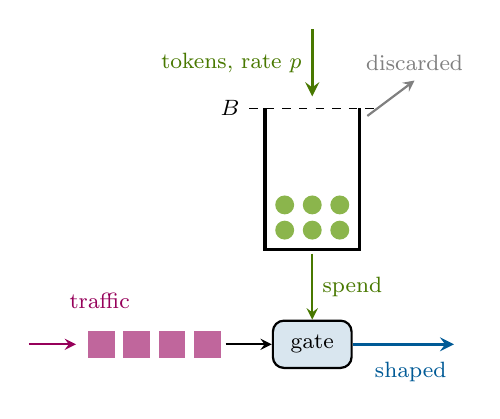
\begin{tikzpicture}[every node/.style={font=\footnotesize}]
				% token source
				\draw[->, very thick, verdecito!80!black] (3.6,4.0) -- node[left] {tokens, rate $p$} (3.6,3.15);
				% bucket
				\draw[very thick] (3.0,3.0) -- (3.0,1.2) -- (4.2,1.2) -- (4.2,3.0);
				\draw[dashed] (2.8,3.0) node[left] {$B$} -- (4.4,3.0);
				\foreach \i in {0,1,2}{ \foreach \j in {0,1}{
					\fill[verdecito!70!white] (3.25+0.35*\i,1.45+0.32*\j) circle (0.12);
				}}
				\draw<3->[->, thick, gray] (4.3,2.9) -- (4.9,3.35) node[above] {discarded};
				% gate
				\node[draw, thick, rounded corners, fill=azulcito!15!white, minimum width=1.0cm, minimum height=0.6cm] (gate) at (3.6,0) {gate};
				\draw[->, thick, verdecito!80!black] (3.6,1.15) -- node[right] {spend} (gate.north);
				% traffic queue
				\node[rojito] at (0.9,0.55) {traffic};
				\draw[->, thick, rojito] (0,0) -- (0.6,0);
				\foreach \k in {0.75,1.2,1.65,2.1}{
					\fill[rojito!60!white] (\k,-0.17) rectangle ++(0.34,0.34);
				}
				\draw[->, thick] (2.5,0) -- (gate.west);
				\draw[->, very thick, azulcito] (gate.east) -- (5.4,0);
				\node[azulcito, below] at (4.85,-0.1) {shaped};
			\end{tikzpicture}
			\end{center}
		\end{column}
	\end{columns}

	\vfill
	\uncover<4->{
	{\footnotesize Introduced to police and shape traffic in ATM and the Internet \cite{Turner1986}; today it is the standard rate limiter of APIs and cloud services.}
	}
\end{frame}

\begin{frame}{Token buckets are fluid queues}

	\begin{myitem}
		\item The token level is a \alert{fluid buffer}: filled at rate $p$, drained by the traffic.
		\item<2-> Token buckets fed by \alert{Markov-modulated} on--off sources were analysed with spectral methods in the early 1990s, e.g.\ \cite{ElwalidMitra1991}.
	\end{myitem}

	\vfill
	\uncover<3->{
	\begin{block}{}
		\begin{center}
		An \alert{old fluid queue}, in a \alert{new setting}: AI agents sharing a token quota.
		\end{center}
	\end{block}
	}
\end{frame}

\begin{frame}{The connection: a shared token bucket}

	\begin{center}
	\renewcommand{\arraystretch}{1.25}
	\begin{tabular}{l|l}
		\alert{token bucket} & \alert{agent fleet}\\\hline
		tokens in the bucket & remaining quota $x$\\
		bucket depth & quota cap $B$\\
		token rate & refill rate $p$\\
		peak rate & burn rate $c$ of an agent\\
		flows arriving & agents activating\\
		empty: held to the token rate & empty: \alert{throttled}\\
		full: tokens discarded & full: refill \alert{wasted}
	\end{tabular}
	\end{center}

	\vfill
	\pause

	The interesting state is the \alert{empty} bucket.
\end{frame}

\begin{frame}{The new setting}

	\begin{block}{}
		\begin{center}
		The quota is a \alert{shared bucket}, drawn on by a \alert{random number of agents} that come and go.\\
		When it runs dry, the agents \alert{finish more slowly}.
		\end{center}
	\end{block}
\end{frame}

\begin{frame}{Key points of this talk}

	\begin{myitem}[1.1em]
		\item A \alert{flow-level model} of a token quota shared by a fleet of on--off agents: a PDMP with state (active agents, tokens left).
		\item All eigenvalues of the stationary problem are \alert{real}: a short proof from reversibility.
		\item The stationary law \alert{exists, is unique and positive}: a $2\times 2$ Perron--Frobenius argument.
		\item \alert{Fluid limit}: the bucket ends full or empty; under-provisioning makes the fleet \alert{pile up}.
		\item \alert{Square-root provisioning} (work in progress): a refill margin of order $\sqrt N$ above the mean burn should need a quota of order $\sqrt N$ only.
	\end{myitem}
\end{frame}

%=====================================================================
\section{The model}
%=====================================================================

\begin{frame}{One agent}

	\begin{myitem}[1em]
		\item An agent is \alert{idle} or \alert{active}. An idle agent starts a task at rate $\lambda$.
		\item A task requires $Y\sim\text{Exp}(\mu)$ \alert{tokens}, drawn afresh each time.
		\item An active agent \alert{burns} tokens at rate $c$ (tokens per unit time).
	\end{myitem}

	\vfill

	\begin{center}
	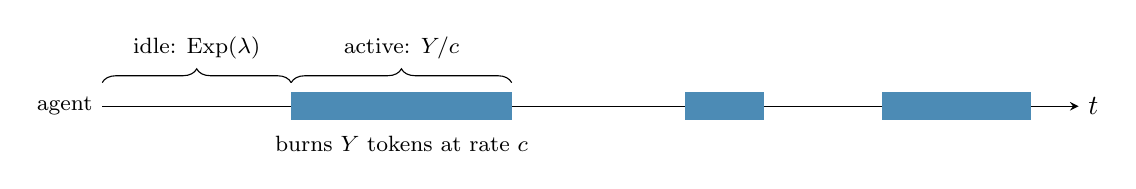
\begin{tikzpicture}
		\draw[->] (0,0) -- (12.4,0) node[right] {$t$};
		\foreach \a/\b in {2.4/5.2, 7.4/8.4, 9.9/11.8}{
			\fill[azulcito!70!white] (\a,-0.18) rectangle (\b,0.18);
		}
		\draw[decorate, decoration={brace, amplitude=5pt}] (0,0.3) -- node[above=5pt] {\footnotesize idle: $\text{Exp}(\lambda)$} (2.4,0.3);
		\draw[decorate, decoration={brace, amplitude=5pt}] (2.4,0.3) -- node[above=5pt] {\footnotesize active: $Y/c$} (5.2,0.3);
		\node[below] at (3.8,-0.25) {\footnotesize burns $Y$ tokens at rate $c$};
		\node[left] at (0,0) {\footnotesize agent};
	\end{tikzpicture}
	\end{center}

	\vfill
\end{frame}

\begin{frame}{One agent: rates}

	\begin{myitem}
		\item The active period is $Y/c\sim\text{Exp}(\nu)$, with \alert{completion rate}
		\begin{equation*}
			\nu := \mu c .
		\end{equation*}
		\item Memoryless demands: the state of an agent is just \alert{idle/active}.
	\end{myitem}

	\vfill
	\pause

	\begin{block}{Notation}
		\begin{equation*}
			\gamma := \lambda+\nu, \qquad \rho := \frac{\lambda}{\gamma} \quad\text{(duty cycle: fraction of time active)}.
		\end{equation*}
	\end{block}
\end{frame}

\begin{frame}{The fleet: an Engset population}

	$N$ agents, independent \alert{as long as tokens remain}. Let $n(t)$ = number of active agents.

	\vfill

	\begin{center}
	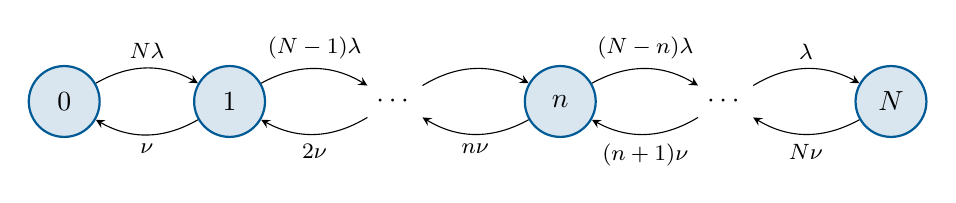
\begin{tikzpicture}[->, >=stealth, node distance=2.1cm, every state/.style={minimum size=0.9cm, fill=azulcito!15!white, draw=azulcito, thick}]
		\node[state] (0) {$0$};
		\node[state, right of=0] (1) {$1$};
		\node[right of=1] (d1) {$\cdots$};
		\node[state, right of=d1] (n) {$n$};
		\node[right of=n] (d2) {$\cdots$};
		\node[state, right of=d2] (N) {$N$};
		\path (0) edge[bend left] node[above] {\footnotesize $N\lambda$} (1)
		      (1) edge[bend left] node[below] {\footnotesize $\nu$} (0)
		      (1) edge[bend left] node[above] {\footnotesize $(N-1)\lambda$} (d1)
		      (d1) edge[bend left] node[below] {\footnotesize $2\nu$} (1)
		      (d1) edge[bend left] node[above] {} (n)
		      (n) edge[bend left] node[below] {\footnotesize $n\nu$} (d1)
		      (n) edge[bend left] node[above] {\footnotesize $(N-n)\lambda$} (d2)
		      (d2) edge[bend left] node[below] {\footnotesize $(n+1)\nu$} (n)
		      (d2) edge[bend left] node[above] {\footnotesize $\lambda$} (N)
		      (N) edge[bend left] node[below] {\footnotesize $N\nu$} (d2);
	\end{tikzpicture}
	\end{center}

	\vfill

	The finite-source birth--death chain of \cite{Engset1918}, with generator $Q$.

	\vfill
\end{frame}

\begin{frame}{The fleet: stationary law}

	\begin{myitem}
		\item Stationary law: \alert{binomial},
		\begin{equation*}
			\pi_n = \binom{N}{n}\rho^n(1-\rho)^{N-n},\qquad N\rho \text{ agents active on average.}
		\end{equation*}
		\item Mean burn rate of the fleet: $c\nb$.
	\end{myitem}

	\vfill
	\pause

	\begin{block}{Reversibility \cite{Kelly1979}}
		\begin{equation*}
			\pi_n\,(N-n)\lambda = \pi_{n+1}\,(n+1)\nu .
		\end{equation*}
		We will use it \alert{twice}: for the spectrum and for positivity.
	\end{block}
\end{frame}

\begin{frame}{The quota}

	\begin{columns}
		\begin{column}{0.55\textwidth}
			\begin{myitem}
				\item Tokens left: $x(t)\in[0,B]$.
				\item The quota \alert{refills} at rate $p$.
				\item With $n$ agents active, the net drift is
				\begin{equation*}
					\dot x = r_n := p - nc .
				\end{equation*}
			\end{myitem}
		\end{column}
		\begin{column}{0.45\textwidth}
			\begin{center}
			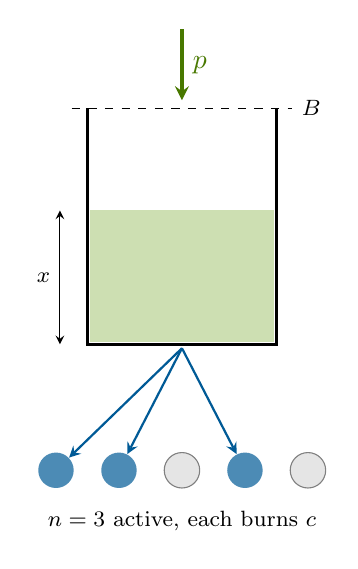
\begin{tikzpicture}
				% bucket
				\draw[very thick] (0,3) -- (0,0) -- (2.4,0) -- (2.4,3);
				\fill[verdecito!30!white] (0.03,0.03) rectangle (2.37,1.7);
				\draw[dashed] (-0.2,3) -- (2.6,3) node[right] {\footnotesize $B$};
				\draw[<->] (-0.35,0) -- node[left] {\footnotesize $x$} (-0.35,1.7);
				\draw[->, very thick, verdecito!80!black] (1.2,4) -- node[right] {$p$} (1.2,3.1);
				% agents
				\foreach \i/\s in {0/1, 1/1, 2/0, 3/1, 4/0}{
					\pgfmathsetmacro{\xx}{-0.4+0.8*\i}
					\ifnum\s=1
						\node[circle, fill=azulcito!70!white, minimum size=0.45cm, inner sep=0pt] (a\i) at (\xx,-1.6) {};
						\draw[->, thick, azulcito] (1.2,-0.05) -- (a\i);
					\else
						\node[circle, draw=gray, fill=gray!20, minimum size=0.45cm, inner sep=0pt] (a\i) at (\xx,-1.6) {};
					\fi
				}
				\node at (1.2,-2.25) {\footnotesize $n=3$ active, each burns $c$};
			\end{tikzpicture}
			\end{center}
		\end{column}
	\end{columns}
\end{frame}

\begin{frame}{Filling and draining modes}

	\begin{myitem}
		\item The drift $r_n=p-nc$ changes sign once, at $\ns := \lfloor p/c\rfloor$:
		\begin{itemize}
			\item $n\leq \ns$: the quota \alert{fills};
			\item $n> \ns$: the quota \alert{drains}.
		\end{itemize}
		\item<2-> Standing assumptions: $0<p<Nc$, and $p/c\notin\mathbb{Z}$, so that no mode has zero drift.
	\end{myitem}

	\vfill
	\uncover<3->{
	\begin{block}{Mean drift $p - c\nb$}
		The plan is \alert{over-provisioned} if $p>c\nb$, \alert{under-provisioned} if $p<c\nb$.
	\end{block}
	}
\end{frame}

\begin{frame}{State space and dynamics}

	\begin{columns}
	\begin{column}{0.52\textwidth}
	\begin{center}
	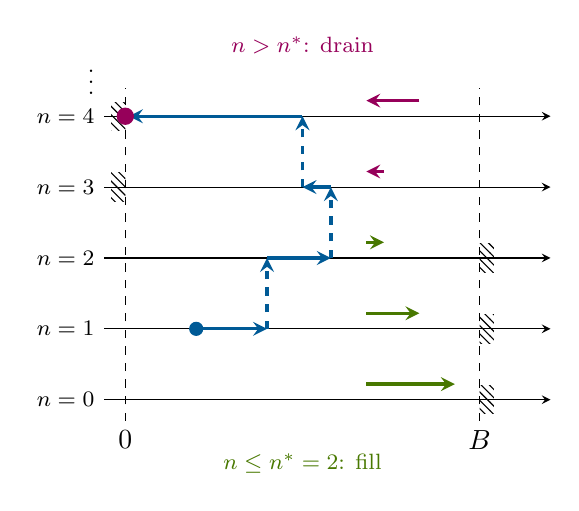
\begin{tikzpicture}[scale=0.9]
		\foreach \n/\y in {0/0, 1/1, 2/2, 3/3, 4/4}{
			\draw[->] (-0.3,\y) node[anchor=east] {\footnotesize $n=\n$} -- (6,\y);
		}
		\node[anchor=east] at (-0.3,4.6) {\footnotesize $\vdots$};
		\draw[dashed] (0,-0.3) node[below] {$0$} -- (0,4.4);
		\draw[dashed] (5,-0.3) node[below] {$B$} -- (5,4.4);
		% drift arrows, length proportional to |r_n| (p/c = 2.5)
		\draw[->, verdecito!80!black, very thick] (3.4,0.22) -- ++(1.25,0);
		\draw[->, verdecito!80!black, very thick] (3.4,1.22) -- ++(0.75,0);
		\draw[->, verdecito!80!black, very thick] (3.4,2.22) -- ++(0.25,0);
		\draw[->, rojito, very thick] (3.65,3.22) -- ++(-0.25,0);
		\draw[->, rojito, very thick] (4.15,4.22) -- ++(-0.75,0);
		\node[verdecito!80!black] at (2.5,-0.9) {\footnotesize $n\le \ns=2$: fill};
		\node[rojito] at (2.5,5.0) {\footnotesize $n> \ns$: drain};
		% sticky barriers
		\foreach \y in {0,1,2}{ \fill[pattern=north west lines] (5,\y-0.2) rectangle ++(.2,.4); }
		\foreach \y in {3,4}{ \fill[pattern=north west lines] (0,\y-0.2) rectangle ++(-.2,.4); }
		% path
		\node[azulcito, fill=azulcito, circle, minimum size=.18cm, inner sep=0pt] at (1,1) {};
		\draw<2->[very thick,azulcito,->] (1,1) -- (2.0,1);
		\draw<3->[very thick,azulcito,dashed,->] (2.0,1) -- (2.0,2);
		\draw<3->[very thick,azulcito,->] (2.0,2) -- (2.9,2);
		\draw<4->[very thick,azulcito,dashed,->] (2.9,2) -- (2.9,3);
		\draw<4->[very thick,azulcito,->] (2.9,3) -- (2.5,3);
		\draw<4->[very thick,azulcito,dashed,->] (2.5,3) -- (2.5,4);
		\draw<4->[very thick,azulcito,->] (2.5,4) -- (0.05,4);
		\node<5->[rojito, fill=rojito, circle, minimum size=.22cm, inner sep=0pt] at (0,4) {};
	\end{tikzpicture}
	\end{center}
	\end{column}
	\begin{column}{0.48\textwidth}
		\begin{itemize}
			\item State: $Z(t)=(n(t),x(t))$.
			\item Arrows: speed $|r_n|$, here $p/c=2.5$.
			\item<2-> Between jumps: $x$ moves \alert{deterministically}; $n$ is frozen.
			\item<3-> Jumps change $n$ by $\pm 1$; $x$ is \alert{unchanged}.
			\item<5-> The flow \alert{reaches the boundary} in finite time, and \alert{sticks} there.
		\end{itemize}
	\end{column}
	\end{columns}
\end{frame}

\begin{frame}{A sample path}

	\begin{center}
		%% Sample path: N=20, lambda=1.0, nu=3.0, c=1.0, p=5.200, B=4.0
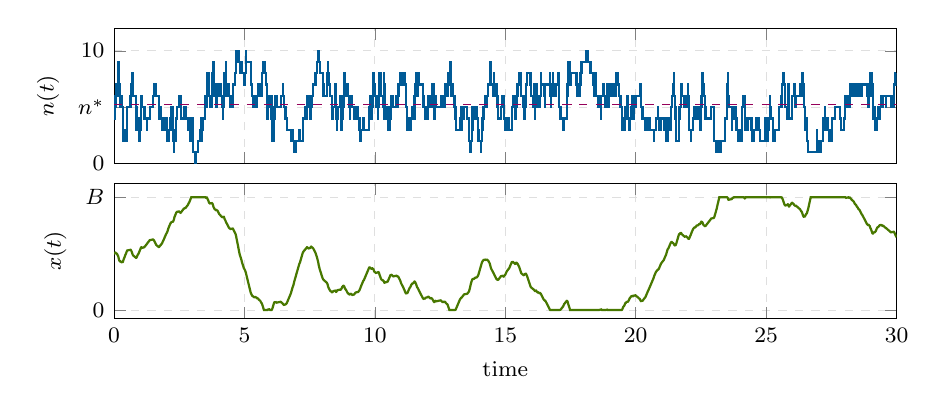
\begin{tikzpicture}
\begin{groupplot}[group style={group size=1 by 2, vertical sep=0.25cm, xlabels at=edge bottom, xticklabels at=edge bottom},
  width=0.95\textwidth, height=3.3cm, xmin=0, xmax=30, grid=major, grid style={gray!25},
  tick label style={font=\footnotesize}, label style={font=\footnotesize}]
\nextgroupplot[ylabel={$n(t)$}, ymin=0, ymax=12, ytick={0,5,10}, yticklabels={0,$n^*$,10}]
\addplot[const plot, azulcito, thick] coordinates {(0.0000,5) (0.0084,5) (0.0084,4) (0.0370,4) (0.0370,5) (0.0519,5) (0.0519,6) (0.0884,6) (0.0884,7) (0.0905,7) (0.0905,6) (0.1164,6) (0.1164,7) (0.1542,7) (0.1542,8) (0.1622,8) (0.1622,9) (0.1936,9) (0.1936,8) (0.2003,8) (0.2003,7) (0.2041,7) (0.2041,6) (0.2302,6) (0.2302,5) (0.2428,5) (0.2428,6) (0.2864,6) (0.2864,5) (0.3350,5) (0.3350,4) (0.3377,4) (0.3377,3) (0.3398,3) (0.3398,2) (0.3642,2) (0.3642,3) (0.4058,3) (0.4058,2) (0.4185,2) (0.4185,3) (0.4753,3) (0.4753,2) (0.4815,2) (0.4815,3) (0.4976,3) (0.4976,4) (0.5055,4) (0.5055,5) (0.6310,5) (0.6310,6) (0.6448,6) (0.6448,7) (0.6730,7) (0.6730,8) (0.7107,8) (0.7107,7) (0.7267,7) (0.7267,6) (0.8385,6) (0.8385,5) (0.8572,5) (0.8572,4) (0.8590,4) (0.8590,3) (0.9023,3) (0.9023,4) (0.9322,4) (0.9322,3) (0.9763,3) (0.9763,2) (0.9813,2) (0.9813,3) (1.0305,3) (1.0305,4) (1.0453,4) (1.0453,5) (1.0488,5) (1.0488,6) (1.0761,6) (1.0761,5) (1.1442,5) (1.1442,4) (1.1659,4) (1.1659,5) (1.1778,5) (1.1778,4) (1.2637,4) (1.2637,3) (1.2664,3) (1.2664,4) (1.3664,4) (1.3664,5) (1.4930,5) (1.4930,6) (1.5262,6) (1.5262,7) (1.6218,7) (1.6218,6) (1.7081,6) (1.7081,5) (1.7272,5) (1.7272,4) (1.7710,4) (1.7710,5) (1.7776,5) (1.7776,4) (1.8392,4) (1.8392,3) (1.8771,3) (1.8771,4) (1.8889,4) (1.8889,3) (1.8934,3) (1.8934,4) (1.8935,4) (1.8935,3) (1.9960,3) (1.9960,4) (2.0156,4) (2.0156,3) (2.0519,3) (2.0519,2) (2.0814,2) (2.0814,3) (2.0858,3) (2.0858,2) (2.0872,2) (2.0872,3) (2.1594,3) (2.1594,4) (2.2024,4) (2.2024,5) (2.2580,5) (2.2580,4) (2.2659,4) (2.2659,3) (2.2821,3) (2.2821,2) (2.2995,2) (2.2995,1) (2.3110,1) (2.3110,2) (2.3172,2) (2.3172,3) (2.3577,3) (2.3577,2) (2.3621,2) (2.3621,3) (2.3827,3) (2.3827,4) (2.4087,4) (2.4087,5) (2.4849,5) (2.4849,6) (2.5469,6) (2.5469,5) (2.5510,5) (2.5510,4) (2.6764,4) (2.6764,5) (2.7048,5) (2.7048,4) (2.7197,4) (2.7197,5) (2.7459,5) (2.7459,4) (2.8338,4) (2.8338,3) (2.8601,3) (2.8601,4) (2.8777,4) (2.8777,3) (2.9277,3) (2.9277,2) (2.9365,2) (2.9365,3) (2.9572,3) (2.9572,4) (2.9574,4) (2.9574,3) (2.9583,3) (2.9601,3) (2.9601,4) (2.9690,4) (2.9690,3) (2.9724,3) (2.9724,4) (3.0108,4) (3.0108,3) (3.0189,3) (3.0189,4) (3.0278,4) (3.0278,3) (3.0280,3) (3.0280,2) (3.0378,2) (3.0378,1) (3.1128,1) (3.1128,0) (3.1469,0) (3.1469,1) (3.2244,1) (3.2244,2) (3.2988,2) (3.2988,3) (3.3166,3) (3.3166,2) (3.3529,2) (3.3529,3) (3.3553,3) (3.3553,4) (3.3734,4) (3.3734,3) (3.4043,3) (3.4043,4) (3.4901,4) (3.4901,5) (3.5015,5) (3.5015,6) (3.5157,6) (3.5157,5) (3.5543,5) (3.5543,6) (3.5608,6) (3.5608,7) (3.5671,7) (3.5671,8) (3.5775,8) (3.5775,7) (3.6146,7) (3.6146,8) (3.6363,8) (3.6363,7) (3.6496,7) (3.6496,6) (3.6727,6) (3.6727,5) (3.7504,5) (3.7504,6) (3.7721,6) (3.7721,7) (3.7734,7) (3.7734,8) (3.7983,8) (3.7983,9) (3.8113,9) (3.8113,8) (3.8114,8) (3.8114,7) (3.8515,7) (3.8515,6) (3.8992,6) (3.8992,5) (3.9280,5) (3.9280,6) (3.9671,6) (3.9671,7) (4.0348,7) (4.0348,6) (4.0729,6) (4.0729,7) (4.0870,7) (4.0870,6) (4.1487,6) (4.1487,5) (4.1712,5) (4.1712,4) (4.1728,4) (4.1728,5) (4.2073,5) (4.2073,6) (4.2096,6) (4.2096,7) (4.2127,7) (4.2127,8) (4.2377,8) (4.2377,7) (4.2774,7) (4.2774,8) (4.2795,8) (4.2795,9) (4.2841,9) (4.2841,8) (4.2939,8) (4.2939,7) (4.2962,7) (4.2962,6) (4.3064,6) (4.3064,7) (4.4020,7) (4.4020,6) (4.4057,6) (4.4057,7) (4.4079,7) (4.4079,6) (4.4610,6) (4.4610,5) (4.5501,5) (4.5501,6) (4.5534,6) (4.5534,7) (4.6491,7) (4.6491,8) (4.6640,8) (4.6640,9) (4.6666,9) (4.6666,8) (4.6707,8) (4.6707,9) (4.6767,9) (4.6767,10) (4.7150,10) (4.7150,9) (4.7187,9) (4.7187,10) (4.7232,10) (4.7232,9) (4.7250,9) (4.7250,10) (4.8037,10) (4.8037,9) (4.8271,9) (4.8271,8) (4.8799,8) (4.8799,9) (4.9129,9) (4.9129,8) (4.9734,8) (4.9734,7) (5.0267,7) (5.0267,8) (5.0458,8) (5.0458,9) (5.0499,9) (5.0499,8) (5.0529,8) (5.0529,9) (5.0610,9) (5.0610,10) (5.0621,10) (5.0621,9) (5.2357,9) (5.2357,8) (5.2460,8) (5.2460,7) (5.2942,7) (5.2942,6) (5.3327,6) (5.3327,5) (5.3404,5) (5.3404,6) (5.3744,6) (5.3744,5) (5.4244,5) (5.4244,6) (5.4757,6) (5.4757,5) (5.4910,5) (5.4910,6) (5.5334,6) (5.5334,7) (5.5421,7) (5.5421,6) (5.6069,6) (5.6069,7) (5.6444,7) (5.6444,6) (5.6528,6) (5.6528,7) (5.6749,7) (5.6749,8) (5.7124,8) (5.7124,9) (5.7242,9) (5.7242,8) (5.7461,8) (5.7884,8) (5.7884,9) (5.8005,9) (5.8005,8) (5.8102,8) (5.8102,7) (5.8148,7) (5.8148,8) (5.8313,8) (5.8313,7) (5.8683,7) (5.8683,6) (5.8702,6) (5.8702,5) (5.8831,5) (5.8831,4) (5.8966,4) (5.8966,5) (5.9487,5) (5.9487,6) (5.9852,6) (6.0330,6) (6.0330,5) (6.0381,5) (6.0381,4) (6.0495,4) (6.0495,3) (6.0727,3) (6.0727,2) (6.1224,2) (6.1224,3) (6.1450,3) (6.1450,4) (6.1477,4) (6.1477,5) (6.1610,5) (6.1610,6) (6.1704,6) (6.1704,5) (6.2065,5) (6.2065,6) (6.2275,6) (6.2275,5) (6.3872,5) (6.3872,6) (6.4639,6) (6.4639,7) (6.4720,7) (6.4720,6) (6.4856,6) (6.4856,7) (6.4897,7) (6.4897,6) (6.5083,6) (6.5083,5) (6.5693,5) (6.5693,4) (6.5811,4) (6.5811,5) (6.5928,5) (6.5928,4) (6.6229,4) (6.6229,3) (6.7749,3) (6.7749,2) (6.8480,2) (6.8480,3) (6.8682,3) (6.8682,2) (6.8863,2) (6.8863,1) (6.9085,1) (6.9085,2) (6.9653,2) (6.9653,1) (6.9702,1) (6.9702,2) (7.1001,2) (7.1001,3) (7.1292,3) (7.1292,2) (7.2309,2) (7.2309,3) (7.2479,3) (7.2479,4) (7.3077,4) (7.3077,5) (7.3118,5) (7.3118,4) (7.3460,4) (7.3460,5) (7.3492,5) (7.3492,4) (7.3949,4) (7.3949,5) (7.4003,5) (7.4003,6) (7.4530,6) (7.4530,5) (7.5096,5) (7.5096,4) (7.5518,4) (7.5518,5) (7.5538,5) (7.5538,6) (7.5956,6) (7.5956,5) (7.6011,5) (7.6011,6) (7.6306,6) (7.6306,7) (7.7200,7) (7.7200,8) (7.7857,8) (7.7857,9) (7.8232,9) (7.8232,10) (7.8488,10) (7.8488,9) (7.8898,9) (7.8898,8) (7.9997,8) (7.9997,7) (8.0148,7) (8.0148,6) (8.0227,6) (8.0227,7) (8.0308,7) (8.0308,6) (8.1558,6) (8.1558,7) (8.1785,7) (8.1785,8) (8.1902,8) (8.1902,9) (8.2033,9) (8.2033,8) (8.2230,8) (8.2230,7) (8.2794,7) (8.2794,6) (8.3536,6) (8.3536,5) (8.3752,5) (8.3752,4) (8.4061,4) (8.4061,5) (8.4833,5) (8.4833,6) (8.4887,6) (8.4887,7) (8.5078,7) (8.5078,6) (8.5138,6) (8.5138,5) (8.5174,5) (8.5174,4) (8.5352,4) (8.5352,3) (8.5394,3) (8.5394,4) (8.5633,4) (8.5633,5) (8.6694,5) (8.6694,6) (8.6769,6) (8.6769,5) (8.6921,5) (8.6921,4) (8.6970,4) (8.6970,3) (8.7004,3) (8.7004,4) (8.7223,4) (8.7223,3) (8.7462,3) (8.7462,4) (8.7814,4) (8.7814,5) (8.7994,5) (8.7994,6) (8.8246,6) (8.8246,7) (8.8252,7) (8.8252,8) (8.8507,8) (8.8507,7) (8.8622,7) (8.8622,6) (8.8857,6) (8.8857,7) (8.9541,7) (8.9541,6) (9.0218,6) (9.0218,5) (9.0397,5) (9.0397,4) (9.0523,4) (9.0523,5) (9.0798,5) (9.0798,6) (9.1016,6) (9.1016,5) (9.1035,5) (9.1035,6) (9.1316,6) (9.1316,5) (9.2006,5) (9.2006,4) (9.2607,4) (9.2607,5) (9.3584,5) (9.3584,4) (9.4055,4) (9.4055,3) (9.4508,3) (9.4508,2) (9.4609,2) (9.4609,3) (9.5538,3) (9.5538,4) (9.5790,4) (9.5790,3) (9.7796,3) (9.7796,4) (9.7805,4) (9.7805,5) (9.8037,5) (9.8037,6) (9.8651,6) (9.8651,5) (9.8714,5) (9.8714,4) (9.8799,4) (9.8799,5) (9.9044,5) (9.9044,6) (9.9425,6) (9.9425,7) (9.9500,7) (9.9500,8) (9.9690,8) (9.9690,7) (9.9817,7) (9.9817,6) (10.0335,6) (10.0335,5) (10.1108,5) (10.1108,4) (10.1159,4) (10.1159,5) (10.1373,5) (10.1373,6) (10.1446,6) (10.1446,7) (10.1554,7) (10.1554,8) (10.1909,8) (10.1909,7) (10.1956,7) (10.1956,8) (10.2202,8) (10.2202,7) (10.2247,7) (10.2247,8) (10.2328,8) (10.2328,7) (10.2428,7) (10.2428,6) (10.2955,6) (10.2955,5) (10.3072,5) (10.3072,6) (10.3389,6) (10.3389,7) (10.3498,7) (10.3498,8) (10.3614,8) (10.3614,7) (10.3653,7) (10.3653,6) (10.3665,6) (10.3665,5) (10.3692,5) (10.3692,4) (10.3772,4) (10.3772,5) (10.4478,5) (10.4478,4) (10.4526,4) (10.4526,5) (10.4597,5) (10.4597,4) (10.4635,4) (10.4635,5) (10.4881,5) (10.4881,4) (10.4928,4) (10.4928,3) (10.5934,3) (10.5934,4) (10.5972,4) (10.5972,5) (10.6392,5) (10.6392,6) (10.7067,6) (10.7067,5) (10.8282,5) (10.8282,6) (10.8597,6) (10.8597,5) (10.8745,5) (10.8745,6) (10.9009,6) (10.9009,7) (10.9674,7) (10.9674,8) (11.0054,8) (11.0054,7) (11.0954,7) (11.0954,8) (11.1080,8) (11.1080,7) (11.1384,7) (11.1384,8) (11.1579,8) (11.1579,7) (11.1787,7) (11.1787,6) (11.1953,6) (11.1953,5) (11.2426,5) (11.2426,4) (11.2508,4) (11.2508,3) (11.3249,3) (11.3249,4) (11.3600,4) (11.3600,3) (11.3961,3) (11.3961,4) (11.4348,4) (11.4348,5) (11.4649,5) (11.4649,4) (11.5197,4) (11.5197,5) (11.5211,5) (11.5211,6) (11.5341,6) (11.5341,7) (11.5710,7) (11.5710,8) (11.6066,8) (11.6066,7) (11.6346,7) (11.6346,6) (11.6430,6) (11.6430,7) (11.6658,7) (11.6658,8) (11.6700,8) (11.6700,7) (11.6956,7) (11.6956,8) (11.6987,8) (11.6987,7) (11.8418,7) (11.8418,6) (11.8634,6) (11.8634,5) (11.9188,5) (11.9188,4) (11.9418,4) (11.9418,5) (12.0152,5) (12.0152,4) (12.0277,4) (12.0277,5) (12.0554,5) (12.0554,6) (12.1279,6) (12.1279,5) (12.1682,5) (12.1682,6) (12.1998,6) (12.1998,7) (12.2543,7) (12.2543,6) (12.2729,6) (12.2729,5) (12.2763,5) (12.2763,4) (12.3114,4) (12.3114,5) (12.3128,5) (12.3128,6) (12.3292,6) (12.3292,5) (12.3434,5) (12.3434,6) (12.3514,6) (12.3514,5) (12.5194,5) (12.5194,6) (12.5931,6) (12.5931,5) (12.6469,5) (12.6469,6) (12.6560,6) (12.6560,5) (12.6737,5) (12.6737,6) (12.6769,6) (12.6769,5) (12.6858,5) (12.6858,6) (12.7082,6) (12.7082,7) (12.7234,7) (12.7234,6) (12.7629,6) (12.7629,7) (12.7657,7) (12.7657,6) (12.7862,6) (12.7862,7) (12.7875,7) (12.7875,8) (12.8559,8) (12.8646,8) (12.8646,7) (12.8669,7) (12.8669,8) (12.8898,8) (12.8898,9) (12.8960,9) (12.8960,8) (12.9025,8) (12.9025,7) (12.9319,7) (12.9319,6) (12.9545,6) (12.9545,7) (12.9881,7) (12.9881,6) (13.0511,6) (13.0511,5) (13.0895,5) (13.0895,4) (13.0965,4) (13.0965,3) (13.2590,3) (13.2590,4) (13.2611,4) (13.2611,3) (13.2641,3) (13.2641,4) (13.3125,4) (13.3125,5) (13.3261,5) (13.3261,4) (13.3433,4) (13.3433,3) (13.3441,3) (13.3441,4) (13.4193,4) (13.4193,5) (13.5424,5) (13.5424,4) (13.6030,4) (13.6030,3) (13.6071,3) (13.6071,2) (13.6386,2) (13.6386,1) (13.6783,1) (13.6783,2) (13.7076,2) (13.7076,3) (13.7391,3) (13.7391,4) (13.7447,4) (13.7447,5) (13.8069,5) (13.8069,4) (13.8323,4) (13.8323,5) (13.8677,5) (13.8677,4) (13.8733,4) (13.8733,5) (13.9090,5) (13.9090,4) (13.9479,4) (13.9479,3) (13.9678,3) (13.9678,2) (14.0764,2) (14.0764,1) (14.0782,1) (14.0782,2) (14.0956,2) (14.0956,3) (14.1238,3) (14.1238,4) (14.1658,4) (14.1658,5) (14.2244,5) (14.2244,6) (14.2370,6) (14.2370,5) (14.2707,5) (14.2707,6) (14.2746,6) (14.2746,5) (14.2997,5) (14.2997,6) (14.3507,6) (14.3507,7) (14.4020,7) (14.4020,8) (14.4107,8) (14.4107,9) (14.4420,9) (14.4420,8) (14.4548,8) (14.4548,7) (14.5456,7) (14.5456,6) (14.5530,6) (14.5530,7) (14.5541,7) (14.5541,8) (14.5642,8) (14.5642,7) (14.6649,7) (14.6649,6) (14.6764,6) (14.6764,5) (14.6873,5) (14.6873,6) (14.7053,6) (14.7053,5) (14.7306,5) (14.7306,4) (14.8352,4) (14.8352,5) (14.8953,5) (14.8953,6) (14.9308,6) (14.9308,5) (14.9413,5) (14.9413,4) (15.0044,4) (15.0044,3) (15.0527,3) (15.0527,4) (15.1495,4) (15.1495,3) (15.2435,3) (15.2435,4) (15.2479,4) (15.2479,5) (15.2897,5) (15.2897,6) (15.3749,6) (15.3749,5) (15.3871,5) (15.3871,4) (15.4173,4) (15.4173,5) (15.4270,5) (15.4270,6) (15.4674,6) (15.4674,7) (15.5275,7) (15.5275,8) (15.6068,8) (15.6068,7) (15.6133,7) (15.6133,6) (15.6970,6) (15.6970,5) (15.7201,5) (15.7201,4) (15.7531,4) (15.7531,5) (15.7891,5) (15.7891,6) (15.7929,6) (15.7929,7) (15.8300,7) (15.8300,8) (15.9663,8) (15.9663,7) (15.9813,7) (15.9813,6) (16.0644,6) (16.0644,5) (16.0680,5) (16.0680,6) (16.1034,6) (16.1034,7) (16.1050,7) (16.1050,6) (16.1133,6) (16.1133,7) (16.1264,7) (16.1264,6) (16.1356,6) (16.1356,5) (16.1448,5) (16.1448,4) (16.1480,4) (16.1480,5) (16.1811,5) (16.1811,6) (16.1924,6) (16.1924,7) (16.2089,7) (16.2089,6) (16.2369,6) (16.2369,5) (16.2600,5) (16.2600,6) (16.3065,6) (16.3065,5) (16.3375,5) (16.3375,6) (16.3566,6) (16.3566,7) (16.3797,7) (16.3797,8) (16.3818,8) (16.3818,7) (16.4791,7) (16.4791,6) (16.5133,6) (16.5133,5) (16.5276,5) (16.5276,6) (16.5322,6) (16.5322,7) (16.6993,7) (16.6993,8) (16.7018,8) (16.7018,7) (16.7114,7) (16.7114,6) (16.7255,6) (16.7498,6) (16.7498,5) (16.7632,5) (16.7632,6) (16.7666,6) (16.7878,6) (16.7878,7) (16.8247,7) (16.8247,8) (16.8280,8) (16.8280,7) (16.8596,7) (16.8596,6) (16.8682,6) (16.8682,7) (16.8956,7) (16.8956,6) (16.9131,6) (16.9131,7) (16.9519,7) (16.9519,6) (16.9557,6) (16.9557,7) (17.0303,7) (17.0303,8) (17.0374,8) (17.0374,7) (17.0516,7) (17.0516,6) (17.0581,6) (17.0581,5) (17.1159,5) (17.1159,4) (17.1394,4) (17.1394,5) (17.1416,5) (17.1416,4) (17.2182,4) (17.2182,3) (17.2521,3) (17.2521,4) (17.3519,4) (17.3519,5) (17.3569,5) (17.3569,6) (17.3842,6) (17.3842,7) (17.3891,7) (17.3891,8) (17.3926,8) (17.3926,9) (17.4115,9) (17.4115,8) (17.4620,8) (17.4620,9) (17.4771,9) (17.4771,8) (17.4830,8) (17.4871,8) (17.4871,7) (17.5291,7) (17.5291,8) (17.7065,8) (17.7065,7) (17.7223,7) (17.7223,8) (17.7452,8) (17.7452,7) (17.7703,7) (17.7703,6) (17.8780,6) (17.8780,7) (17.8853,7) (17.8853,8) (17.9224,8) (17.9224,9) (18.1041,9) (18.1041,10) (18.1844,10) (18.1844,9) (18.2652,9) (18.2652,8) (18.3798,8) (18.3798,7) (18.3981,7) (18.3981,6) (18.3987,6) (18.3987,7) (18.4322,7) (18.4322,6) (18.4359,6) (18.4359,7) (18.4723,7) (18.4723,8) (18.4773,8) (18.4773,7) (18.4846,7) (18.4846,6) (18.5742,6) (18.5742,5) (18.6580,5) (18.6580,4) (18.6602,4) (18.6602,5) (18.6788,5) (18.6788,6) (18.7078,6) (18.7361,6) (18.7361,7) (18.7586,7) (18.7586,6) (18.7749,6) (18.7749,7) (18.7970,7) (18.7970,6) (18.8293,6) (18.8293,5) (18.9054,5) (18.9054,6) (18.9204,6) (18.9204,7) (18.9222,7) (18.9298,7) (18.9298,6) (18.9332,6) (18.9332,7) (18.9486,7) (18.9486,6) (18.9552,6) (18.9552,5) (18.9640,5) (18.9640,6) (18.9646,6) (18.9646,5) (18.9793,5) (18.9793,6) (18.9846,6) (18.9864,6) (18.9864,7) (19.0343,7) (19.0343,6) (19.0606,6) (19.0606,7) (19.0928,7) (19.0928,6) (19.1067,6) (19.1067,7) (19.1287,7) (19.1287,6) (19.2230,6) (19.2230,7) (19.2540,7) (19.2540,8) (19.3163,8) (19.3163,7) (19.3534,7) (19.3534,6) (19.3972,6) (19.3972,5) (19.4064,5) (19.4064,6) (19.4087,6) (19.4389,6) (19.4389,5) (19.4724,5) (19.4724,4) (19.4760,4) (19.4760,3) (19.5211,3) (19.5211,4) (19.5616,4) (19.5616,3) (19.6008,3) (19.6008,4) (19.6070,4) (19.6070,5) (19.6217,5) (19.6217,4) (19.6488,4) (19.6488,5) (19.6827,5) (19.6827,6) (19.6835,6) (19.6835,5) (19.6957,5) (19.6957,4) (19.7325,4) (19.7325,3) (19.7653,3) (19.7653,4) (19.8278,4) (19.8278,5) (19.8385,5) (19.8385,4) (19.8432,4) (19.8432,5) (19.8788,5) (19.8788,6) (19.8937,6) (19.8937,5) (19.9058,5) (19.9058,4) (19.9122,4) (19.9122,5) (19.9231,5) (19.9231,4) (19.9317,4) (19.9317,5) (19.9843,5) (19.9843,6) (20.0085,6) (20.0085,5) (20.0145,5) (20.0145,6) (20.1540,6) (20.1540,7) (20.1936,7) (20.1936,6) (20.1997,6) (20.1997,5) (20.2617,5) (20.2617,4) (20.3724,4) (20.3724,3) (20.4745,3) (20.4745,4) (20.4837,4) (20.4837,3) (20.5395,3) (20.5395,4) (20.5420,4) (20.5420,3) (20.6882,3) (20.6882,2) (20.7068,2) (20.7068,3) (20.7718,3) (20.7718,4) (20.8409,4) (20.8409,5) (20.8630,5) (20.8630,4) (20.8856,4) (20.8856,3) (20.9721,3) (20.9721,4) (21.0748,4) (21.0748,3) (21.1343,3) (21.1343,4) (21.1375,4) (21.1375,3) (21.1653,3) (21.1653,2) (21.2203,2) (21.2203,3) (21.2221,3) (21.2221,4) (21.2526,4) (21.2526,3) (21.3409,3) (21.3409,4) (21.3666,4) (21.3666,5) (21.3799,5) (21.3799,6) (21.4400,6) (21.4400,7) (21.4459,7) (21.4459,6) (21.4614,6) (21.4614,7) (21.4698,7) (21.4698,8) (21.4726,8) (21.4726,7) (21.4770,7) (21.4770,6) (21.4992,6) (21.4992,5) (21.5273,5) (21.5273,4) (21.5313,4) (21.5313,3) (21.5535,3) (21.5535,2) (21.6523,2) (21.6523,3) (21.6576,3) (21.6576,4) (21.6667,4) (21.6667,5) (21.6846,5) (21.6846,4) (21.7106,4) (21.7106,5) (21.7364,5) (21.7364,6) (21.7468,6) (21.7468,7) (21.7676,7) (21.7676,6) (21.8734,6) (21.8734,5) (21.9290,5) (21.9290,6) (21.9915,6) (21.9915,7) (22.0015,7) (22.0015,6) (22.0205,6) (22.0205,5) (22.0241,5) (22.0241,6) (22.0306,6) (22.0306,5) (22.0393,5) (22.0393,4) (22.0517,4) (22.0517,3) (22.1114,3) (22.1114,2) (22.1186,2) (22.1186,3) (22.1967,3) (22.1967,4) (22.2413,4) (22.2413,5) (22.2814,5) (22.2814,4) (22.3363,4) (22.3363,5) (22.3952,5) (22.3952,4) (22.4247,4) (22.4247,5) (22.4605,5) (22.4605,4) (22.4785,4) (22.4785,3) (22.4958,3) (22.4958,4) (22.5138,4) (22.5138,5) (22.5239,5) (22.5239,6) (22.5576,6) (22.5576,7) (22.5614,7) (22.5614,8) (22.5834,8) (22.5834,7) (22.5872,7) (22.5872,6) (22.5990,6) (22.5990,7) (22.6027,7) (22.6027,6) (22.6504,6) (22.6504,5) (22.6775,5) (22.6775,4) (22.8976,4) (22.8976,5) (22.9916,5) (22.9916,4) (23.0048,4) (23.0048,3) (23.0129,3) (23.0129,2) (23.0761,2) (23.0761,1) (23.0806,1) (23.0806,2) (23.1035,2) (23.1035,1) (23.1463,1) (23.1463,2) (23.1580,2) (23.1580,1) (23.2025,1) (23.2098,1) (23.2098,2) (23.2687,2) (23.2687,1) (23.2698,1) (23.2698,2) (23.4195,2) (23.4195,3) (23.4302,3) (23.4302,4) (23.4849,4) (23.4849,5) (23.5047,5) (23.5047,6) (23.5213,6) (23.5213,7) (23.5301,7) (23.5301,8) (23.5461,8) (23.5461,7) (23.5497,7) (23.5497,6) (23.5585,6) (23.5585,5) (23.6809,5) (23.6809,4) (23.6823,4) (23.6823,3) (23.6837,3) (23.6837,4) (23.7170,4) (23.7170,5) (23.7597,5) (23.7597,4) (23.7678,4) (23.8380,4) (23.8380,5) (23.8386,5) (23.8386,4) (23.8473,4) (23.8473,3) (23.8599,3) (23.8599,4) (23.8941,4) (23.8941,3) (23.9401,3) (23.9401,2) (23.9694,2) (23.9694,3) (24.0582,3) (24.0582,2) (24.0734,2) (24.0734,3) (24.0777,3) (24.0777,4) (24.0889,4) (24.0889,5) (24.1354,5) (24.1354,6) (24.1823,6) (24.1823,5) (24.1895,5) (24.1895,4) (24.1913,4) (24.1913,3) (24.2007,3) (24.2007,4) (24.2107,4) (24.2107,3) (24.2113,3) (24.2905,3) (24.2905,4) (24.4047,4) (24.4047,3) (24.4339,3) (24.4339,4) (24.4355,4) (24.4355,3) (24.4505,3) (24.4505,2) (24.5321,2) (24.5321,3) (24.6290,3) (24.6290,4) (24.6404,4) (24.6404,3) (24.6647,3) (24.6647,4) (24.7103,4) (24.7103,3) (24.7515,3) (24.7515,2) (24.9453,2) (24.9453,3) (24.9655,3) (24.9655,4) (24.9939,4) (24.9939,3) (25.0011,3) (25.0011,4) (25.0094,4) (25.0094,3) (25.0488,3) (25.0488,2) (25.0785,2) (25.0785,3) (25.0939,3) (25.0939,4) (25.1466,4) (25.1466,5) (25.1523,5) (25.1523,6) (25.1561,6) (25.1561,5) (25.1712,5) (25.1775,5) (25.1775,4) (25.2701,4) (25.2701,3) (25.2813,3) (25.2813,2) (25.3392,2) (25.3392,3) (25.4957,3) (25.4957,4) (25.5011,4) (25.5011,5) (25.5791,5) (25.5791,6) (25.5915,6) (25.5915,5) (25.6003,5) (25.6003,6) (25.6031,6) (25.6031,7) (25.6324,7) (25.6324,8) (25.6932,8) (25.6932,7) (25.7159,7) (25.7159,6) (25.7352,6) (25.7352,5) (25.8029,5) (25.8029,4) (25.8268,4) (25.8268,5) (25.8287,5) (25.8287,6) (25.8364,6) (25.8364,7) (25.8763,7) (25.8763,6) (25.8764,6) (25.8764,5) (25.8789,5) (25.8789,4) (25.9852,4) (25.9852,5) (25.9972,5) (25.9972,6) (26.0595,6) (26.0595,7) (26.0723,7) (26.0723,6) (26.0891,6) (26.0891,7) (26.0899,7) (26.0899,6) (26.1226,6) (26.1226,5) (26.1491,5) (26.1491,6) (26.3046,6) (26.3046,7) (26.3384,7) (26.3384,6) (26.3556,6) (26.3556,7) (26.3730,7) (26.3730,8) (26.4102,8) (26.4102,7) (26.4371,7) (26.4371,6) (26.4393,6) (26.4393,5) (26.4817,5) (26.4817,4) (26.4997,4) (26.4997,3) (26.5200,3) (26.5200,4) (26.5571,4) (26.5571,3) (26.5684,3) (26.5684,2) (26.6107,2) (26.6107,1) (26.7079,1) (26.9412,1) (26.9412,2) (26.9458,2) (26.9458,3) (26.9496,3) (26.9496,2) (27.0393,2) (27.0393,1) (27.0856,1) (27.0856,2) (27.1687,2) (27.1687,3) (27.2007,3) (27.2007,4) (27.2487,4) (27.2487,5) (27.2546,5) (27.2546,4) (27.2716,4) (27.2716,3) (27.2799,3) (27.2799,4) (27.3338,4) (27.3338,3) (27.3498,3) (27.3498,4) (27.3701,4) (27.3701,3) (27.4094,3) (27.4094,2) (27.4232,2) (27.4232,3) (27.4425,3) (27.4425,2) (27.4777,2) (27.4777,3) (27.4782,3) (27.4782,2) (27.5235,2) (27.5235,3) (27.5391,3) (27.5391,4) (27.6303,4) (27.6303,5) (27.8459,5) (27.8459,4) (27.8818,4) (27.8818,3) (27.9774,3) (27.9774,4) (28.0370,4) (28.0370,5) (28.0421,5) (28.0421,6) (28.0646,6) (28.0646,5) (28.1199,5) (28.1199,6) (28.1202,6) (28.1202,5) (28.1561,5) (28.1573,5) (28.1573,6) (28.1750,6) (28.1750,5) (28.2096,5) (28.2096,6) (28.2226,6) (28.2226,7) (28.2329,7) (28.2329,6) (28.2569,6) (28.2569,7) (28.2701,7) (28.2701,6) (28.3545,6) (28.3545,7) (28.4042,7) (28.4042,6) (28.4462,6) (28.4462,7) (28.4854,7) (28.4854,6) (28.5064,6) (28.5064,7) (28.5372,7) (28.5372,6) (28.5764,6) (28.5764,7) (28.6671,7) (28.6671,6) (28.6841,6) (28.6841,7) (28.8679,7) (28.8679,6) (28.9063,6) (28.9063,5) (28.9330,5) (28.9330,6) (28.9363,6) (28.9363,7) (28.9479,7) (28.9479,6) (28.9670,6) (28.9670,7) (28.9767,7) (28.9767,8) (28.9993,8) (28.9993,7) (29.0081,7) (29.0081,6) (29.0110,6) (29.0110,7) (29.0218,7) (29.0218,8) (29.0648,8) (29.0648,7) (29.0745,7) (29.0745,6) (29.0915,6) (29.0915,5) (29.0939,5) (29.0939,4) (29.1270,4) (29.1270,5) (29.1686,5) (29.1686,4) (29.1722,4) (29.1722,3) (29.1733,3) (29.1733,4) (29.2027,4) (29.2027,3) (29.2511,3) (29.2511,4) (29.2758,4) (29.2758,5) (29.2969,5) (29.2969,4) (29.3496,4) (29.3496,5) (29.4048,5) (29.4048,6) (29.4298,6) (29.4298,5) (29.4530,5) (29.4530,6) (29.4745,6) (29.4745,5) (29.4890,5) (29.4890,6) (29.5958,6) (29.5958,5) (29.6004,5) (29.6004,6) (29.7834,6) (29.7834,5) (29.8303,5) (29.8303,6) (29.8331,6) (29.8331,5) (29.8967,5) (29.8967,6) (29.9020,6) (29.9020,7) (29.9363,7) (29.9363,8) (29.9529,8) (29.9529,7) (29.9989,7) (29.9989,8)};
\addplot[dashed, rojito, domain=0:30] {5.2000};
\nextgroupplot[ylabel={$x(t)$}, xlabel={time}, ymin=-0.3, ymax=4.5, ytick={0,4}, yticklabels={0,$B$}]
\addplot[verdecito!80!black, thick] coordinates {(0.0000,2.0000) (0.0084,2.0017) (0.0084,2.0017) (0.0370,2.0360) (0.0370,2.0360) (0.0519,2.0390) (0.0519,2.0390) (0.0884,2.0098) (0.0884,2.0098) (0.0905,2.0059) (0.0905,2.0059) (0.1164,1.9852) (0.1164,1.9852) (0.1542,1.9173) (0.1542,1.9173) (0.1622,1.8949) (0.1622,1.8949) (0.1936,1.7756) (0.1936,1.7756) (0.2003,1.7568) (0.2003,1.7568) (0.2041,1.7500) (0.2041,1.7500) (0.2302,1.7291) (0.2302,1.7291) (0.2428,1.7316) (0.2428,1.7316) (0.2864,1.6967) (0.2864,1.6967) (0.3350,1.7064) (0.3350,1.7064) (0.3377,1.7096) (0.3377,1.7096) (0.3398,1.7142) (0.3398,1.7142) (0.3642,1.7924) (0.3642,1.7924) (0.4058,1.8839) (0.4058,1.8839) (0.4185,1.9246) (0.4185,1.9246) (0.4753,2.0495) (0.4753,2.0495) (0.4815,2.0695) (0.4815,2.0695) (0.4976,2.1048) (0.4976,2.1048) (0.5055,2.1143) (0.5055,2.1143) (0.6310,2.1394) (0.6310,2.1394) (0.6448,2.1284) (0.6448,2.1284) (0.6730,2.0776) (0.6730,2.0776) (0.7107,1.9721) (0.7107,1.9721) (0.7267,1.9433) (0.7267,1.9433) (0.8385,1.8538) (0.8385,1.8538) (0.8572,1.8576) (0.8572,1.8576) (0.8590,1.8597) (0.8590,1.8597) (0.9023,1.9550) (0.9023,1.9550) (0.9322,1.9908) (0.9322,1.9908) (0.9763,2.0879) (0.9763,2.0879) (0.9813,2.1039) (0.9813,2.1039) (1.0305,2.2120) (1.0305,2.2120) (1.0453,2.2298) (1.0453,2.2298) (1.0488,2.2305) (1.0488,2.2305) (1.0761,2.2086) (1.0761,2.2086) (1.1442,2.2222) (1.1442,2.2222) (1.1659,2.2483) (1.1659,2.2483) (1.1778,2.2507) (1.1778,2.2507) (1.2637,2.3538) (1.2637,2.3538) (1.2664,2.3598) (1.2664,2.3598) (1.3664,2.4798) (1.3664,2.4798) (1.4930,2.5051) (1.4930,2.5051) (1.5262,2.4785) (1.5262,2.4785) (1.6218,2.3063) (1.6218,2.3063) (1.7081,2.2373) (1.7081,2.2373) (1.7272,2.2412) (1.7272,2.2412) (1.7710,2.2936) (1.7710,2.2936) (1.7776,2.2950) (1.7776,2.2950) (1.8392,2.3689) (1.8392,2.3689) (1.8771,2.4522) (1.8771,2.4522) (1.8889,2.4664) (1.8889,2.4664) (1.8934,2.4764) (1.8934,2.4764) (1.8935,2.4765) (1.8935,2.4765) (1.9960,2.7019) (1.9960,2.7019) (2.0156,2.7254) (2.0156,2.7254) (2.0519,2.8054) (2.0519,2.8054) (2.0814,2.8997) (2.0814,2.8997) (2.0858,2.9094) (2.0858,2.9094) (2.0872,2.9139) (2.0872,2.9139) (2.1594,3.0727) (2.1594,3.0727) (2.2024,3.1244) (2.2024,3.1244) (2.2580,3.1355) (2.2580,3.1355) (2.2659,3.1449) (2.2659,3.1449) (2.2821,3.1807) (2.2821,3.1807) (2.2995,3.2363) (2.2995,3.2363) (2.3110,3.2846) (2.3110,3.2846) (2.3172,3.3043) (2.3172,3.3043) (2.3577,3.3934) (2.3577,3.3934) (2.3621,3.4074) (2.3621,3.4074) (2.3827,3.4527) (2.3827,3.4527) (2.4087,3.4840) (2.4087,3.4840) (2.4849,3.4992) (2.4849,3.4992) (2.5469,3.4495) (2.5469,3.4495) (2.5510,3.4503) (2.5510,3.4503) (2.6764,3.6008) (2.6764,3.6008) (2.7048,3.6065) (2.7048,3.6065) (2.7197,3.6244) (2.7197,3.6244) (2.7459,3.6297) (2.7459,3.6297) (2.8338,3.7351) (2.8338,3.7351) (2.8601,3.7930) (2.8601,3.7930) (2.8777,3.8141) (2.8777,3.8141) (2.9277,3.9240) (2.9277,3.9240) (2.9365,3.9524) (2.9365,3.9524) (2.9572,3.9978) (2.9572,3.9978) (2.9574,3.9981) (2.9574,3.9981) (2.9583,4.0000) (2.9601,4.0000) (2.9601,4.0000) (2.9690,4.0000) (2.9690,4.0000) (2.9724,4.0000) (2.9724,4.0000) (3.0108,4.0000) (3.0108,4.0000) (3.0189,4.0000) (3.0189,4.0000) (3.0278,4.0000) (3.0278,4.0000) (3.0280,4.0000) (3.0280,4.0000) (3.0378,4.0000) (3.0378,4.0000) (3.1128,4.0000) (3.1128,4.0000) (3.1469,4.0000) (3.1469,4.0000) (3.2244,4.0000) (3.2244,4.0000) (3.2988,4.0000) (3.2988,4.0000) (3.3166,4.0000) (3.3166,4.0000) (3.3529,4.0000) (3.3529,4.0000) (3.3553,4.0000) (3.3553,4.0000) (3.3734,4.0000) (3.3734,4.0000) (3.4043,4.0000) (3.4043,4.0000) (3.4901,4.0000) (3.4901,4.0000) (3.5015,4.0000) (3.5015,4.0000) (3.5157,3.9887) (3.5157,3.9887) (3.5543,3.9964) (3.5543,3.9964) (3.5608,3.9912) (3.5608,3.9912) (3.5671,3.9800) (3.5671,3.9800) (3.5775,3.9509) (3.5775,3.9509) (3.6146,3.8840) (3.6146,3.8840) (3.6363,3.8234) (3.6363,3.8234) (3.6496,3.7994) (3.6496,3.7994) (3.6727,3.7810) (3.6727,3.7810) (3.7504,3.7965) (3.7504,3.7965) (3.7721,3.7791) (3.7721,3.7791) (3.7734,3.7768) (3.7734,3.7768) (3.7983,3.7070) (3.7983,3.7070) (3.8113,3.6578) (3.8113,3.6578) (3.8114,3.6574) (3.8114,3.6574) (3.8515,3.5852) (3.8515,3.5852) (3.8992,3.5471) (3.8992,3.5471) (3.9280,3.5529) (3.9280,3.5529) (3.9671,3.5216) (3.9671,3.5216) (4.0348,3.3997) (4.0348,3.3997) (4.0729,3.3692) (4.0729,3.3692) (4.0870,3.3439) (4.0870,3.3439) (4.1487,3.2946) (4.1487,3.2946) (4.1712,3.2991) (4.1712,3.2991) (4.1728,3.3010) (4.1728,3.3010) (4.2073,3.3079) (4.2073,3.3079) (4.2096,3.3061) (4.2096,3.3061) (4.2127,3.3005) (4.2127,3.3005) (4.2377,3.2305) (4.2377,3.2305) (4.2774,3.1590) (4.2774,3.1590) (4.2795,3.1531) (4.2795,3.1531) (4.2841,3.1358) (4.2841,3.1358) (4.2939,3.1083) (4.2939,3.1083) (4.2962,3.1042) (4.2962,3.1042) (4.3064,3.0960) (4.3064,3.0960) (4.4020,2.9240) (4.4020,2.9240) (4.4057,2.9210) (4.4057,2.9210) (4.4079,2.9171) (4.4079,2.9171) (4.4610,2.8746) (4.4610,2.8746) (4.5501,2.8924) (4.5501,2.8924) (4.5534,2.8898) (4.5534,2.8898) (4.6491,2.7175) (4.6491,2.7175) (4.6640,2.6758) (4.6640,2.6758) (4.6666,2.6657) (4.6666,2.6657) (4.6707,2.6544) (4.6707,2.6544) (4.6767,2.6315) (4.6767,2.6315) (4.7150,2.4478) (4.7150,2.4478) (4.7187,2.4337) (4.7187,2.4337) (4.7232,2.4121) (4.7232,2.4121) (4.7250,2.4053) (4.7250,2.4053) (4.8037,2.0272) (4.8037,2.0272) (4.8271,1.9386) (4.8271,1.9386) (4.8799,1.7908) (4.8799,1.7908) (4.9129,1.6651) (4.9129,1.6651) (4.9734,1.4959) (4.9734,1.4959) (5.0267,1.4000) (5.0267,1.4000) (5.0458,1.3465) (5.0458,1.3465) (5.0499,1.3309) (5.0499,1.3309) (5.0529,1.3225) (5.0529,1.3225) (5.0610,1.2914) (5.0610,1.2914) (5.0621,1.2863) (5.0621,1.2863) (5.2357,0.6266) (5.2357,0.6266) (5.2460,0.5976) (5.2460,0.5976) (5.2942,0.5109) (5.2942,0.5109) (5.3327,0.4802) (5.3327,0.4802) (5.3404,0.4817) (5.3404,0.4817) (5.3744,0.4546) (5.3744,0.4546) (5.4244,0.4646) (5.4244,0.4646) (5.4757,0.4235) (5.4757,0.4235) (5.4910,0.4266) (5.4910,0.4266) (5.5334,0.3927) (5.5334,0.3927) (5.5421,0.3770) (5.5421,0.3770) (5.6069,0.3252) (5.6069,0.3252) (5.6444,0.2578) (5.6444,0.2578) (5.6528,0.2511) (5.6528,0.2511) (5.6749,0.2113) (5.6749,0.2113) (5.7124,0.1063) (5.7124,0.1063) (5.7242,0.0611) (5.7242,0.0611) (5.7461,0.0000) (5.7884,0.0000) (5.7884,0.0000) (5.8005,0.0000) (5.8005,0.0000) (5.8102,0.0000) (5.8102,0.0000) (5.8148,0.0000) (5.8148,0.0000) (5.8313,0.0000) (5.8313,0.0000) (5.8683,0.0000) (5.8683,0.0000) (5.8702,0.0000) (5.8702,0.0000) (5.8831,0.0026) (5.8831,0.0026) (5.8966,0.0188) (5.8966,0.0188) (5.9487,0.0292) (5.9487,0.0292) (5.9852,0.0000) (6.0330,0.0000) (6.0330,0.0000) (6.0381,0.0010) (6.0381,0.0010) (6.0495,0.0147) (6.0495,0.0147) (6.0727,0.0656) (6.0727,0.0656) (6.1224,0.2246) (6.1224,0.2246) (6.1450,0.2745) (6.1450,0.2745) (6.1477,0.2777) (6.1477,0.2777) (6.1610,0.2804) (6.1610,0.2804) (6.1704,0.2728) (6.1704,0.2728) (6.2065,0.2801) (6.2065,0.2801) (6.2275,0.2633) (6.2275,0.2633) (6.3872,0.2952) (6.3872,0.2952) (6.4639,0.2338) (6.4639,0.2338) (6.4720,0.2193) (6.4720,0.2193) (6.4856,0.2084) (6.4856,0.2084) (6.4897,0.2011) (6.4897,0.2011) (6.5083,0.1862) (6.5083,0.1862) (6.5693,0.1984) (6.5693,0.1984) (6.5811,0.2126) (6.5811,0.2126) (6.5928,0.2149) (6.5928,0.2149) (6.6229,0.2511) (6.6229,0.2511) (6.7749,0.5853) (6.7749,0.5853) (6.8480,0.8193) (6.8480,0.8193) (6.8682,0.8637) (6.8682,0.8637) (6.8863,0.9218) (6.8863,0.9218) (6.9085,1.0149) (6.9085,1.0149) (6.9653,1.1967) (6.9653,1.1967) (6.9702,1.2173) (6.9702,1.2173) (7.1001,1.6328) (7.1001,1.6328) (7.1292,1.6970) (7.1292,1.6970) (7.2309,2.0225) (7.2309,2.0225) (7.2479,2.0597) (7.2479,2.0597) (7.3077,2.1315) (7.3077,2.1315) (7.3118,2.1323) (7.3118,2.1323) (7.3460,2.1734) (7.3460,2.1734) (7.3492,2.1740) (7.3492,2.1740) (7.3949,2.2289) (7.3949,2.2289) (7.4003,2.2300) (7.4003,2.2300) (7.4530,2.1878) (7.4530,2.1878) (7.5096,2.1991) (7.5096,2.1991) (7.5518,2.2497) (7.5518,2.2497) (7.5538,2.2501) (7.5538,2.2501) (7.5956,2.2167) (7.5956,2.2167) (7.6011,2.2179) (7.6011,2.2179) (7.6306,2.1943) (7.6306,2.1943) (7.7200,2.0333) (7.7200,2.0333) (7.7857,1.8494) (7.7857,1.8494) (7.8232,1.7069) (7.8232,1.7069) (7.8488,1.5839) (7.8488,1.5839) (7.8898,1.4281) (7.8898,1.4281) (7.9997,1.1205) (7.9997,1.1205) (8.0148,1.0933) (8.0148,1.0933) (8.0227,1.0870) (8.0227,1.0870) (8.0308,1.0723) (8.0308,1.0723) (8.1558,0.9724) (8.1558,0.9724) (8.1785,0.9315) (8.1785,0.9315) (8.1902,0.8987) (8.1902,0.8987) (8.2033,0.8490) (8.2033,0.8490) (8.2230,0.7938) (8.2230,0.7938) (8.2794,0.6922) (8.2794,0.6922) (8.3536,0.6329) (8.3536,0.6329) (8.3752,0.6372) (8.3752,0.6372) (8.4061,0.6743) (8.4061,0.6743) (8.4833,0.6897) (8.4833,0.6897) (8.4887,0.6854) (8.4887,0.6854) (8.5078,0.6509) (8.5078,0.6509) (8.5138,0.6462) (8.5138,0.6462) (8.5174,0.6469) (8.5174,0.6469) (8.5352,0.6682) (8.5352,0.6682) (8.5394,0.6774) (8.5394,0.6774) (8.5633,0.7061) (8.5633,0.7061) (8.6694,0.7273) (8.6694,0.7273) (8.6769,0.7213) (8.6769,0.7213) (8.6921,0.7244) (8.6921,0.7244) (8.6970,0.7303) (8.6970,0.7303) (8.7004,0.7377) (8.7004,0.7377) (8.7223,0.7640) (8.7223,0.7640) (8.7462,0.8165) (8.7462,0.8165) (8.7814,0.8587) (8.7814,0.8587) (8.7994,0.8623) (8.7994,0.8623) (8.8246,0.8422) (8.8246,0.8422) (8.8252,0.8410) (8.8252,0.8410) (8.8507,0.7698) (8.8507,0.7698) (8.8622,0.7491) (8.8622,0.7491) (8.8857,0.7303) (8.8857,0.7303) (8.9541,0.6070) (8.9541,0.6070) (9.0218,0.5529) (9.0218,0.5529) (9.0397,0.5565) (9.0397,0.5565) (9.0523,0.5717) (9.0523,0.5717) (9.0798,0.5772) (9.0798,0.5772) (9.1016,0.5598) (9.1016,0.5598) (9.1035,0.5602) (9.1035,0.5602) (9.1316,0.5377) (9.1316,0.5377) (9.2006,0.5515) (9.2006,0.5515) (9.2607,0.6237) (9.2607,0.6237) (9.3584,0.6433) (9.3584,0.6433) (9.4055,0.6998) (9.4055,0.6998) (9.4508,0.7994) (9.4508,0.7994) (9.4609,0.8316) (9.4609,0.8316) (9.5538,1.0360) (9.5538,1.0360) (9.5790,1.0663) (9.5790,1.0663) (9.7796,1.5076) (9.7796,1.5076) (9.7805,1.5087) (9.7805,1.5087) (9.8037,1.5134) (9.8037,1.5134) (9.8651,1.4643) (9.8651,1.4643) (9.8714,1.4655) (9.8714,1.4655) (9.8799,1.4758) (9.8799,1.4758) (9.9044,1.4807) (9.9044,1.4807) (9.9425,1.4502) (9.9425,1.4502) (9.9500,1.4368) (9.9500,1.4368) (9.9690,1.3835) (9.9690,1.3835) (9.9817,1.3607) (9.9817,1.3607) (10.0335,1.3192) (10.0335,1.3192) (10.1108,1.3347) (10.1108,1.3347) (10.1159,1.3407) (10.1159,1.3407) (10.1373,1.3450) (10.1373,1.3450) (10.1446,1.3392) (10.1446,1.3392) (10.1554,1.3197) (10.1554,1.3197) (10.1909,1.2202) (10.1909,1.2202) (10.1956,1.2119) (10.1956,1.2119) (10.2202,1.1428) (10.2202,1.1428) (10.2247,1.1348) (10.2247,1.1348) (10.2328,1.1120) (10.2328,1.1120) (10.2428,1.0940) (10.2428,1.0940) (10.2955,1.0519) (10.2955,1.0519) (10.3072,1.0542) (10.3072,1.0542) (10.3389,1.0288) (10.3389,1.0288) (10.3498,1.0093) (10.3498,1.0093) (10.3614,0.9768) (10.3614,0.9768) (10.3653,0.9697) (10.3653,0.9697) (10.3665,0.9687) (10.3665,0.9687) (10.3692,0.9693) (10.3692,0.9693) (10.3772,0.9789) (10.3772,0.9789) (10.4478,0.9930) (10.4478,0.9930) (10.4526,0.9987) (10.4526,0.9987) (10.4597,1.0001) (10.4597,1.0001) (10.4635,1.0047) (10.4635,1.0047) (10.4881,1.0096) (10.4881,1.0096) (10.4928,1.0153) (10.4928,1.0153) (10.5934,1.2365) (10.5934,1.2365) (10.5972,1.2412) (10.5972,1.2412) (10.6392,1.2495) (10.6392,1.2495) (10.7067,1.1955) (10.7067,1.1955) (10.8282,1.2198) (10.8282,1.2198) (10.8597,1.1946) (10.8597,1.1946) (10.8745,1.1975) (10.8745,1.1975) (10.9009,1.1764) (10.9009,1.1764) (10.9674,1.0568) (10.9674,1.0568) (11.0054,0.9503) (11.0054,0.9503) (11.0954,0.7883) (11.0954,0.7883) (11.1080,0.7529) (11.1080,0.7529) (11.1384,0.6983) (11.1384,0.6983) (11.1579,0.6436) (11.1579,0.6436) (11.1787,0.6061) (11.1787,0.6061) (11.1953,0.5929) (11.1953,0.5929) (11.2426,0.6023) (11.2426,0.6023) (11.2508,0.6122) (11.2508,0.6122) (11.3249,0.7753) (11.3249,0.7753) (11.3600,0.8174) (11.3600,0.8174) (11.3961,0.8969) (11.3961,0.8969) (11.4348,0.9433) (11.4348,0.9433) (11.4649,0.9494) (11.4649,0.9494) (11.5197,1.0151) (11.5197,1.0151) (11.5211,1.0154) (11.5211,1.0154) (11.5341,1.0050) (11.5341,1.0050) (11.5710,0.9385) (11.5710,0.9385) (11.6066,0.8388) (11.6066,0.8388) (11.6346,0.7885) (11.6346,0.7885) (11.6430,0.7817) (11.6430,0.7817) (11.6658,0.7406) (11.6658,0.7406) (11.6700,0.7290) (11.6700,0.7290) (11.6956,0.6829) (11.6956,0.6829) (11.6987,0.6744) (11.6987,0.6744) (11.8418,0.4167) (11.8418,0.4167) (11.8634,0.3994) (11.8634,0.3994) (11.9188,0.4105) (11.9188,0.4105) (11.9418,0.4381) (11.9418,0.4381) (12.0152,0.4528) (12.0152,0.4528) (12.0277,0.4677) (12.0277,0.4677) (12.0554,0.4732) (12.0554,0.4732) (12.1279,0.4152) (12.1279,0.4152) (12.1682,0.4232) (12.1682,0.4232) (12.1998,0.3980) (12.1998,0.3980) (12.2543,0.2998) (12.2543,0.2998) (12.2729,0.2849) (12.2729,0.2849) (12.2763,0.2856) (12.2763,0.2856) (12.3114,0.3277) (12.3114,0.3277) (12.3128,0.3280) (12.3128,0.3280) (12.3292,0.3148) (12.3292,0.3148) (12.3434,0.3177) (12.3434,0.3177) (12.3514,0.3112) (12.3514,0.3112) (12.5194,0.3448) (12.5194,0.3448) (12.5931,0.2859) (12.5931,0.2859) (12.6469,0.2966) (12.6469,0.2966) (12.6560,0.2894) (12.6560,0.2894) (12.6737,0.2929) (12.6737,0.2929) (12.6769,0.2904) (12.6769,0.2904) (12.6858,0.2921) (12.6858,0.2921) (12.7082,0.2742) (12.7082,0.2742) (12.7234,0.2469) (12.7234,0.2469) (12.7629,0.2153) (12.7629,0.2153) (12.7657,0.2103) (12.7657,0.2103) (12.7862,0.1939) (12.7862,0.1939) (12.7875,0.1916) (12.7875,0.1916) (12.8559,0.0000) (12.8646,0.0000) (12.8646,0.0000) (12.8669,0.0000) (12.8669,0.0000) (12.8898,0.0000) (12.8898,0.0000) (12.8960,0.0000) (12.8960,0.0000) (12.9025,0.0000) (12.9025,0.0000) (12.9319,0.0000) (12.9319,0.0000) (12.9545,0.0000) (12.9545,0.0000) (12.9881,0.0000) (12.9881,0.0000) (13.0511,0.0000) (13.0511,0.0000) (13.0895,0.0077) (13.0895,0.0077) (13.0965,0.0161) (13.0965,0.0161) (13.2590,0.3735) (13.2590,0.3735) (13.2611,0.3760) (13.2611,0.3760) (13.2641,0.3827) (13.2641,0.3827) (13.3125,0.4408) (13.3125,0.4408) (13.3261,0.4435) (13.3261,0.4435) (13.3433,0.4642) (13.3433,0.4642) (13.3441,0.4660) (13.3441,0.4660) (13.4193,0.5562) (13.4193,0.5562) (13.5424,0.5808) (13.5424,0.5808) (13.6030,0.6536) (13.6030,0.6536) (13.6071,0.6626) (13.6071,0.6626) (13.6386,0.7633) (13.6386,0.7633) (13.6783,0.9300) (13.6783,0.9300) (13.7076,1.0238) (13.7076,1.0238) (13.7391,1.0930) (13.7391,1.0930) (13.7447,1.0998) (13.7447,1.0998) (13.8069,1.1122) (13.8069,1.1122) (13.8323,1.1427) (13.8323,1.1427) (13.8677,1.1498) (13.8677,1.1498) (13.8733,1.1565) (13.8733,1.1565) (13.9090,1.1637) (13.9090,1.1637) (13.9479,1.2104) (13.9479,1.2104) (13.9678,1.2542) (13.9678,1.2542) (14.0764,1.6016) (14.0764,1.6016) (14.0782,1.6091) (14.0782,1.6091) (14.0956,1.6649) (14.0956,1.6649) (14.1238,1.7269) (14.1238,1.7269) (14.1658,1.7773) (14.1658,1.7773) (14.2244,1.7891) (14.2244,1.7891) (14.2370,1.7790) (14.2370,1.7790) (14.2707,1.7857) (14.2707,1.7857) (14.2746,1.7826) (14.2746,1.7826) (14.2997,1.7876) (14.2997,1.7876) (14.3507,1.7469) (14.3507,1.7469) (14.4020,1.6545) (14.4020,1.6545) (14.4107,1.6300) (14.4107,1.6300) (14.4420,1.5114) (14.4420,1.5114) (14.4548,1.4753) (14.4548,1.4753) (14.5456,1.3120) (14.5456,1.3120) (14.5530,1.3061) (14.5530,1.3061) (14.5541,1.3040) (14.5541,1.3040) (14.5642,1.2759) (14.5642,1.2759) (14.6649,1.0946) (14.6649,1.0946) (14.6764,1.0853) (14.6764,1.0853) (14.6873,1.0875) (14.6873,1.0875) (14.7053,1.0730) (14.7053,1.0730) (14.7306,1.0781) (14.7306,1.0781) (14.8352,1.2036) (14.8352,1.2036) (14.8953,1.2156) (14.8953,1.2156) (14.9308,1.1872) (14.9308,1.1872) (14.9413,1.1893) (14.9413,1.1893) (15.0044,1.2650) (15.0044,1.2650) (15.0527,1.3713) (15.0527,1.3713) (15.1495,1.4875) (15.1495,1.4875) (15.2435,1.6942) (15.2435,1.6942) (15.2479,1.6994) (15.2479,1.6994) (15.2897,1.7078) (15.2897,1.7078) (15.3749,1.6396) (15.3749,1.6396) (15.3871,1.6420) (15.3871,1.6420) (15.4173,1.6782) (15.4173,1.6782) (15.4270,1.6802) (15.4270,1.6802) (15.4674,1.6478) (15.4674,1.6478) (15.5275,1.5396) (15.5275,1.5396) (15.6068,1.3178) (15.6068,1.3178) (15.6133,1.3060) (15.6133,1.3060) (15.6970,1.2391) (15.6970,1.2391) (15.7201,1.2437) (15.7201,1.2437) (15.7531,1.2833) (15.7531,1.2833) (15.7891,1.2905) (15.7891,1.2905) (15.7929,1.2874) (15.7929,1.2874) (15.8300,1.2206) (15.8300,1.2206) (15.9663,0.8389) (15.9663,0.8389) (15.9813,0.8119) (15.9813,0.8119) (16.0644,0.7455) (16.0644,0.7455) (16.0680,0.7462) (16.0680,0.7462) (16.1034,0.7179) (16.1034,0.7179) (16.1050,0.7151) (16.1050,0.7151) (16.1133,0.7084) (16.1133,0.7084) (16.1264,0.6849) (16.1264,0.6849) (16.1356,0.6775) (16.1356,0.6775) (16.1448,0.6793) (16.1448,0.6793) (16.1480,0.6832) (16.1480,0.6832) (16.1811,0.6898) (16.1811,0.6898) (16.1924,0.6807) (16.1924,0.6807) (16.2089,0.6511) (16.2089,0.6511) (16.2369,0.6287) (16.2369,0.6287) (16.2600,0.6333) (16.2600,0.6333) (16.3065,0.5961) (16.3065,0.5961) (16.3375,0.6023) (16.3375,0.6023) (16.3566,0.5871) (16.3566,0.5871) (16.3797,0.5455) (16.3797,0.5455) (16.3818,0.5396) (16.3818,0.5396) (16.4791,0.3644) (16.4791,0.3644) (16.5133,0.3371) (16.5133,0.3371) (16.5276,0.3399) (16.5276,0.3399) (16.5322,0.3362) (16.5322,0.3362) (16.6993,0.0354) (16.6993,0.0354) (16.7018,0.0286) (16.7018,0.0286) (16.7114,0.0113) (16.7114,0.0113) (16.7255,0.0000) (16.7498,0.0000) (16.7498,0.0000) (16.7632,0.0027) (16.7632,0.0027) (16.7666,0.0000) (16.7878,0.0000) (16.7878,0.0000) (16.8247,0.0000) (16.8247,0.0000) (16.8280,0.0000) (16.8280,0.0000) (16.8596,0.0000) (16.8596,0.0000) (16.8682,0.0000) (16.8682,0.0000) (16.8956,0.0000) (16.8956,0.0000) (16.9131,0.0000) (16.9131,0.0000) (16.9519,0.0000) (16.9519,0.0000) (16.9557,0.0000) (16.9557,0.0000) (17.0303,0.0000) (17.0303,0.0000) (17.0374,0.0000) (17.0374,0.0000) (17.0516,0.0000) (17.0516,0.0000) (17.0581,0.0000) (17.0581,0.0000) (17.1159,0.0116) (17.1159,0.0116) (17.1394,0.0398) (17.1394,0.0398) (17.1416,0.0402) (17.1416,0.0402) (17.2182,0.1322) (17.2182,0.1322) (17.2521,0.2068) (17.2521,0.2068) (17.3519,0.3266) (17.3519,0.3266) (17.3569,0.3275) (17.3569,0.3275) (17.3842,0.3057) (17.3842,0.3057) (17.3891,0.2967) (17.3891,0.2967) (17.3926,0.2869) (17.3926,0.2869) (17.4115,0.2153) (17.4115,0.2153) (17.4620,0.0740) (17.4620,0.0740) (17.4771,0.0164) (17.4771,0.0164) (17.4830,0.0000) (17.4871,0.0000) (17.4871,0.0000) (17.5291,0.0000) (17.5291,0.0000) (17.7065,0.0000) (17.7065,0.0000) (17.7223,0.0000) (17.7223,0.0000) (17.7452,0.0000) (17.7452,0.0000) (17.7703,0.0000) (17.7703,0.0000) (17.8780,0.0000) (17.8780,0.0000) (17.8853,0.0000) (17.8853,0.0000) (17.9224,0.0000) (17.9224,0.0000) (18.1041,0.0000) (18.1041,0.0000) (18.1844,0.0000) (18.1844,0.0000) (18.2652,0.0000) (18.2652,0.0000) (18.3798,0.0000) (18.3798,0.0000) (18.3981,0.0000) (18.3981,0.0000) (18.3987,0.0000) (18.3987,0.0000) (18.4322,0.0000) (18.4322,0.0000) (18.4359,0.0000) (18.4359,0.0000) (18.4723,0.0000) (18.4723,0.0000) (18.4773,0.0000) (18.4773,0.0000) (18.4846,0.0000) (18.4846,0.0000) (18.5742,0.0000) (18.5742,0.0000) (18.6580,0.0168) (18.6580,0.0168) (18.6602,0.0194) (18.6602,0.0194) (18.6788,0.0231) (18.6788,0.0231) (18.7078,0.0000) (18.7361,0.0000) (18.7361,0.0000) (18.7586,0.0000) (18.7586,0.0000) (18.7749,0.0000) (18.7749,0.0000) (18.7970,0.0000) (18.7970,0.0000) (18.8293,0.0000) (18.8293,0.0000) (18.9054,0.0152) (18.9054,0.0152) (18.9204,0.0032) (18.9204,0.0032) (18.9222,0.0000) (18.9298,0.0000) (18.9298,0.0000) (18.9332,0.0000) (18.9332,0.0000) (18.9486,0.0000) (18.9486,0.0000) (18.9552,0.0000) (18.9552,0.0000) (18.9640,0.0018) (18.9640,0.0018) (18.9646,0.0013) (18.9646,0.0013) (18.9793,0.0042) (18.9793,0.0042) (18.9846,0.0000) (18.9864,0.0000) (18.9864,0.0000) (19.0343,0.0000) (19.0343,0.0000) (19.0606,0.0000) (19.0606,0.0000) (19.0928,0.0000) (19.0928,0.0000) (19.1067,0.0000) (19.1067,0.0000) (19.1287,0.0000) (19.1287,0.0000) (19.2230,0.0000) (19.2230,0.0000) (19.2540,0.0000) (19.2540,0.0000) (19.3163,0.0000) (19.3163,0.0000) (19.3534,0.0000) (19.3534,0.0000) (19.3972,0.0000) (19.3972,0.0000) (19.4064,0.0018) (19.4064,0.0018) (19.4087,0.0000) (19.4389,0.0000) (19.4389,0.0000) (19.4724,0.0067) (19.4724,0.0067) (19.4760,0.0110) (19.4760,0.0110) (19.5211,0.1102) (19.5211,0.1102) (19.5616,0.1589) (19.5616,0.1589) (19.6008,0.2451) (19.6008,0.2451) (19.6070,0.2525) (19.6070,0.2525) (19.6217,0.2554) (19.6217,0.2554) (19.6488,0.2879) (19.6488,0.2879) (19.6827,0.2947) (19.6827,0.2947) (19.6835,0.2941) (19.6835,0.2941) (19.6957,0.2965) (19.6957,0.2965) (19.7325,0.3407) (19.7325,0.3407) (19.7653,0.4130) (19.7653,0.4130) (19.8278,0.4879) (19.8278,0.4879) (19.8385,0.4900) (19.8385,0.4900) (19.8432,0.4956) (19.8432,0.4956) (19.8788,0.5027) (19.8788,0.5027) (19.8937,0.4908) (19.8937,0.4908) (19.9058,0.4932) (19.9058,0.4932) (19.9122,0.5009) (19.9122,0.5009) (19.9231,0.5031) (19.9231,0.5031) (19.9317,0.5134) (19.9317,0.5134) (19.9843,0.5239) (19.9843,0.5239) (20.0085,0.5046) (20.0085,0.5046) (20.0145,0.5058) (20.0145,0.5058) (20.1540,0.3942) (20.1540,0.3942) (20.1936,0.3228) (20.1936,0.3228) (20.1997,0.3179) (20.1997,0.3179) (20.2617,0.3303) (20.2617,0.3303) (20.3724,0.4631) (20.3724,0.4631) (20.4745,0.6878) (20.4745,0.6878) (20.4837,0.6988) (20.4837,0.6988) (20.5395,0.8216) (20.5395,0.8216) (20.5420,0.8245) (20.5420,0.8245) (20.6882,1.1463) (20.6882,1.1463) (20.7068,1.2056) (20.7068,1.2056) (20.7718,1.3487) (20.7718,1.3487) (20.8409,1.4316) (20.8409,1.4316) (20.8630,1.4360) (20.8630,1.4360) (20.8856,1.4631) (20.8856,1.4631) (20.9721,1.6533) (20.9721,1.6533) (21.0748,1.7766) (21.0748,1.7766) (21.1343,1.9074) (21.1343,1.9074) (21.1375,1.9113) (21.1375,1.9113) (21.1653,1.9724) (21.1653,1.9724) (21.2203,2.1483) (21.2203,2.1483) (21.2221,2.1523) (21.2221,2.1523) (21.2526,2.1889) (21.2526,2.1889) (21.3409,2.3830) (21.3409,2.3830) (21.3666,2.4139) (21.3666,2.4139) (21.3799,2.4166) (21.3799,2.4166) (21.4400,2.3685) (21.4400,2.3685) (21.4459,2.3580) (21.4459,2.3580) (21.4614,2.3456) (21.4614,2.3456) (21.4698,2.3304) (21.4698,2.3304) (21.4726,2.3226) (21.4726,2.3226) (21.4770,2.3146) (21.4770,2.3146) (21.4992,2.2968) (21.4992,2.2968) (21.5273,2.3025) (21.5273,2.3025) (21.5313,2.3073) (21.5313,2.3073) (21.5535,2.3562) (21.5535,2.3562) (21.6523,2.6724) (21.6523,2.6724) (21.6576,2.6840) (21.6576,2.6840) (21.6667,2.6949) (21.6667,2.6949) (21.6846,2.6985) (21.6846,2.6985) (21.7106,2.7296) (21.7106,2.7296) (21.7364,2.7348) (21.7364,2.7348) (21.7468,2.7265) (21.7468,2.7265) (21.7676,2.6890) (21.7676,2.6890) (21.8734,2.6045) (21.8734,2.6045) (21.9290,2.6156) (21.9290,2.6156) (21.9915,2.5655) (21.9915,2.5655) (22.0015,2.5475) (22.0015,2.5475) (22.0205,2.5324) (22.0205,2.5324) (22.0241,2.5331) (22.0241,2.5331) (22.0306,2.5280) (22.0306,2.5280) (22.0393,2.5297) (22.0393,2.5297) (22.0517,2.5446) (22.0517,2.5446) (22.1114,2.6759) (22.1114,2.6759) (22.1186,2.6989) (22.1186,2.6989) (22.1967,2.8707) (22.1967,2.8707) (22.2413,2.9243) (22.2413,2.9243) (22.2814,2.9323) (22.2814,2.9323) (22.3363,2.9982) (22.3363,2.9982) (22.3952,3.0100) (22.3952,3.0100) (22.4247,3.0454) (22.4247,3.0454) (22.4605,3.0525) (22.4605,3.0525) (22.4785,3.0741) (22.4785,3.0741) (22.4958,3.1123) (22.4958,3.1123) (22.5138,3.1338) (22.5138,3.1338) (22.5239,3.1359) (22.5239,3.1359) (22.5576,3.1089) (22.5576,3.1089) (22.5614,3.1021) (22.5614,3.1021) (22.5834,3.0406) (22.5834,3.0406) (22.5872,3.0336) (22.5872,3.0336) (22.5990,3.0242) (22.5990,3.0242) (22.6027,3.0176) (22.6027,3.0176) (22.6504,2.9795) (22.6504,2.9795) (22.6775,2.9849) (22.6775,2.9849) (22.8976,3.2490) (22.8976,3.2490) (22.9916,3.2678) (22.9916,3.2678) (23.0048,3.2837) (23.0048,3.2837) (23.0129,3.3014) (23.0129,3.3014) (23.0761,3.5038) (23.0761,3.5038) (23.0806,3.5227) (23.0806,3.5227) (23.1035,3.5960) (23.1035,3.5960) (23.1463,3.7759) (23.1463,3.7759) (23.1580,3.8131) (23.1580,3.8131) (23.2025,4.0000) (23.2098,4.0000) (23.2098,4.0000) (23.2687,4.0000) (23.2687,4.0000) (23.2698,4.0000) (23.2698,4.0000) (23.4195,4.0000) (23.4195,4.0000) (23.4302,4.0000) (23.4302,4.0000) (23.4849,4.0000) (23.4849,4.0000) (23.5047,4.0000) (23.5047,4.0000) (23.5213,3.9867) (23.5213,3.9867) (23.5301,3.9709) (23.5301,3.9709) (23.5461,3.9261) (23.5461,3.9261) (23.5497,3.9195) (23.5497,3.9195) (23.5585,3.9125) (23.5585,3.9125) (23.6809,3.9370) (23.6809,3.9370) (23.6823,3.9387) (23.6823,3.9387) (23.6837,3.9418) (23.6837,3.9418) (23.7170,3.9817) (23.7170,3.9817) (23.7597,3.9902) (23.7597,3.9902) (23.7678,4.0000) (23.8380,4.0000) (23.8380,4.0000) (23.8386,4.0000) (23.8386,4.0000) (23.8473,4.0000) (23.8473,4.0000) (23.8599,4.0000) (23.8599,4.0000) (23.8941,4.0000) (23.8941,4.0000) (23.9401,4.0000) (23.9401,4.0000) (23.9694,4.0000) (23.9694,4.0000) (24.0582,4.0000) (24.0582,4.0000) (24.0734,4.0000) (24.0734,4.0000) (24.0777,4.0000) (24.0777,4.0000) (24.0889,4.0000) (24.0889,4.0000) (24.1354,4.0000) (24.1354,4.0000) (24.1823,3.9625) (24.1823,3.9625) (24.1895,3.9639) (24.1895,3.9639) (24.1913,3.9660) (24.1913,3.9660) (24.2007,3.9867) (24.2007,3.9867) (24.2107,3.9987) (24.2107,3.9987) (24.2113,4.0000) (24.2905,4.0000) (24.2905,4.0000) (24.4047,4.0000) (24.4047,4.0000) (24.4339,4.0000) (24.4339,4.0000) (24.4355,4.0000) (24.4355,4.0000) (24.4505,4.0000) (24.4505,4.0000) (24.5321,4.0000) (24.5321,4.0000) (24.6290,4.0000) (24.6290,4.0000) (24.6404,4.0000) (24.6404,4.0000) (24.6647,4.0000) (24.6647,4.0000) (24.7103,4.0000) (24.7103,4.0000) (24.7515,4.0000) (24.7515,4.0000) (24.9453,4.0000) (24.9453,4.0000) (24.9655,4.0000) (24.9655,4.0000) (24.9939,4.0000) (24.9939,4.0000) (25.0011,4.0000) (25.0011,4.0000) (25.0094,4.0000) (25.0094,4.0000) (25.0488,4.0000) (25.0488,4.0000) (25.0785,4.0000) (25.0785,4.0000) (25.0939,4.0000) (25.0939,4.0000) (25.1466,4.0000) (25.1466,4.0000) (25.1523,4.0000) (25.1523,4.0000) (25.1561,3.9970) (25.1561,3.9970) (25.1712,4.0000) (25.1775,4.0000) (25.1775,4.0000) (25.2701,4.0000) (25.2701,4.0000) (25.2813,4.0000) (25.2813,4.0000) (25.3392,4.0000) (25.3392,4.0000) (25.4957,4.0000) (25.4957,4.0000) (25.5011,4.0000) (25.5011,4.0000) (25.5791,4.0000) (25.5791,4.0000) (25.5915,3.9901) (25.5915,3.9901) (25.6003,3.9919) (25.6003,3.9919) (25.6031,3.9896) (25.6031,3.9896) (25.6324,3.9369) (25.6324,3.9369) (25.6932,3.7667) (25.6932,3.7667) (25.7159,3.7258) (25.7159,3.7258) (25.7352,3.7103) (25.7352,3.7103) (25.8029,3.7238) (25.8029,3.7238) (25.8268,3.7525) (25.8268,3.7525) (25.8287,3.7529) (25.8287,3.7529) (25.8364,3.7467) (25.8364,3.7467) (25.8763,3.6749) (25.8763,3.6749) (25.8764,3.6749) (25.8764,3.6749) (25.8789,3.6754) (25.8789,3.6754) (25.9852,3.8030) (25.9852,3.8030) (25.9972,3.8054) (25.9972,3.8054) (26.0595,3.7555) (26.0595,3.7555) (26.0723,3.7324) (26.0723,3.7324) (26.0891,3.7191) (26.0891,3.7191) (26.0899,3.7176) (26.0899,3.7176) (26.1226,3.6914) (26.1226,3.6914) (26.1491,3.6967) (26.1491,3.6967) (26.3046,3.5723) (26.3046,3.5723) (26.3384,3.5115) (26.3384,3.5115) (26.3556,3.4977) (26.3556,3.4977) (26.3730,3.4665) (26.3730,3.4665) (26.4102,3.3623) (26.4102,3.3623) (26.4371,3.3139) (26.4371,3.3139) (26.4393,3.3121) (26.4393,3.3121) (26.4817,3.3206) (26.4817,3.3206) (26.4997,3.3422) (26.4997,3.3422) (26.5200,3.3870) (26.5200,3.3870) (26.5571,3.4314) (26.5571,3.4314) (26.5684,3.4563) (26.5684,3.4563) (26.6107,3.5918) (26.6107,3.5918) (26.7079,4.0000) (26.9412,4.0000) (26.9412,4.0000) (26.9458,4.0000) (26.9458,4.0000) (26.9496,4.0000) (26.9496,4.0000) (27.0393,4.0000) (27.0393,4.0000) (27.0856,4.0000) (27.0856,4.0000) (27.1687,4.0000) (27.1687,4.0000) (27.2007,4.0000) (27.2007,4.0000) (27.2487,4.0000) (27.2487,4.0000) (27.2546,4.0000) (27.2546,4.0000) (27.2716,4.0000) (27.2716,4.0000) (27.2799,4.0000) (27.2799,4.0000) (27.3338,4.0000) (27.3338,4.0000) (27.3498,4.0000) (27.3498,4.0000) (27.3701,4.0000) (27.3701,4.0000) (27.4094,4.0000) (27.4094,4.0000) (27.4232,4.0000) (27.4232,4.0000) (27.4425,4.0000) (27.4425,4.0000) (27.4777,4.0000) (27.4777,4.0000) (27.4782,4.0000) (27.4782,4.0000) (27.5235,4.0000) (27.5235,4.0000) (27.5391,4.0000) (27.5391,4.0000) (27.6303,4.0000) (27.6303,4.0000) (27.8459,4.0000) (27.8459,4.0000) (27.8818,4.0000) (27.8818,4.0000) (27.9774,4.0000) (27.9774,4.0000) (28.0370,4.0000) (28.0370,4.0000) (28.0421,4.0000) (28.0421,4.0000) (28.0646,3.9820) (28.0646,3.9820) (28.1199,3.9930) (28.1199,3.9930) (28.1202,3.9928) (28.1202,3.9928) (28.1561,4.0000) (28.1573,4.0000) (28.1573,4.0000) (28.1750,3.9858) (28.1750,3.9858) (28.2096,3.9928) (28.2096,3.9928) (28.2226,3.9824) (28.2226,3.9824) (28.2329,3.9639) (28.2329,3.9639) (28.2569,3.9447) (28.2569,3.9447) (28.2701,3.9209) (28.2701,3.9209) (28.3545,3.8534) (28.3545,3.8534) (28.4042,3.7640) (28.4042,3.7640) (28.4462,3.7304) (28.4462,3.7304) (28.4854,3.6597) (28.4854,3.6597) (28.5064,3.6429) (28.5064,3.6429) (28.5372,3.5874) (28.5372,3.5874) (28.5764,3.5561) (28.5764,3.5561) (28.6671,3.3929) (28.6671,3.3929) (28.6841,3.3793) (28.6841,3.3793) (28.8679,3.0484) (28.8679,3.0484) (28.9063,3.0177) (28.9063,3.0177) (28.9330,3.0230) (28.9330,3.0230) (28.9363,3.0204) (28.9363,3.0204) (28.9479,2.9994) (28.9479,2.9994) (28.9670,2.9842) (28.9670,2.9842) (28.9767,2.9668) (28.9767,2.9668) (28.9993,2.9035) (28.9993,2.9035) (29.0081,2.8876) (29.0081,2.8876) (29.0110,2.8852) (29.0110,2.8852) (29.0218,2.8659) (29.0218,2.8659) (29.0648,2.7455) (29.0648,2.7455) (29.0745,2.7280) (29.0745,2.7280) (29.0915,2.7144) (29.0915,2.7144) (29.0939,2.7149) (29.0939,2.7149) (29.1270,2.7546) (29.1270,2.7546) (29.1686,2.7629) (29.1686,2.7629) (29.1722,2.7672) (29.1722,2.7672) (29.1733,2.7696) (29.1733,2.7696) (29.2027,2.8049) (29.2027,2.8049) (29.2511,2.9113) (29.2511,2.9113) (29.2758,2.9410) (29.2758,2.9410) (29.2969,2.9453) (29.2969,2.9453) (29.3496,3.0085) (29.3496,3.0085) (29.4048,3.0196) (29.4048,3.0196) (29.4298,2.9995) (29.4298,2.9995) (29.4530,3.0041) (29.4530,3.0041) (29.4745,2.9870) (29.4745,2.9870) (29.4890,2.9899) (29.4890,2.9899) (29.5958,2.9044) (29.5958,2.9044) (29.6004,2.9053) (29.6004,2.9053) (29.7834,2.7590) (29.7834,2.7590) (29.8303,2.7684) (29.8303,2.7684) (29.8331,2.7662) (29.8331,2.7662) (29.8967,2.7789) (29.8967,2.7789) (29.9020,2.7747) (29.9020,2.7747) (29.9363,2.7130) (29.9363,2.7130) (29.9529,2.6664) (29.9529,2.6664) (29.9989,2.5836) (29.9989,2.5836)};
\end{groupplot}
\end{tikzpicture}

	\end{center}

	\vfill
	{\footnotesize $N=20$, $\rho=0.25$ ($\nb=5$), $c=1$, refill $p=5.2$, $B=4$. Long run: quota empty $9\%$ of the time, full $15\%$, in between $76\%$.}
\end{frame}

\begin{frame}{The full bucket}

	\begin{myitem}
		\item If $x=B$ and $n\leq \ns$, the refill would push the quota above its cap: the excess is \alert{discarded}.
		\item The quota \alert{sticks} at $B$; the agents are \alert{unaffected}.
		\item It leaves $B$ when the fleet crosses to $n=\ns+1$.
	\end{myitem}

	\vfill
	\pause

	\begin{myitem}
		\item \alert{Atoms} of the stationary law at $(n,B)$, $n\leq\ns$.
		\item \alert{Wasted refill rate}: $\displaystyle W = \sum_{n\le \ns} (p-nc)\,P(n=n,\ x=B)$.
	\end{myitem}
\end{frame}

\begin{frame}{The empty bucket}

	\begin{myitem}
		\item If $x=0$ and $n>\ns$, the agents want $nc$ tokens per unit time, but only $p$ arrive.
		\item<2-> \alert{Tokens are the unit of work}: a task is done when its $Y$ tokens have been burnt.
		\item<3-> A starved agent does not slow down a stream: it \alert{stops progressing}.
	\end{myitem}
\end{frame}

\begin{frame}{The empty bucket: throttling}

	The $p$ incoming tokens are \alert{shared} among the $n$ active agents: each burns at rate $p/n$, and completes at rate $\mu p/n$.

	\vfill
	\pause

	\begin{block}{Completion rate of the fleet}
		\begin{equation*}
			m(n,x) = \begin{cases} n\nu & x>0 \text{ or } n\leq\ns,\\ \mu p & x=0,\ n>\ns \quad\text{(\alert{throttled})}.\end{cases}
		\end{equation*}
	\end{block}

	\vfill
	\pause

	\begin{myitem}[1em]
		\item Activations continue at $(N-n)\lambda$; the quota stays at $0$ until $n$ drops to $\ns$.
		\item Work is \alert{conserved}: no task is lost, the fleet just progresses at the refill rate.
		\item At $x=0$ the fleet's rates depend on the quota: the chain $n(t)$ is \alert{not autonomous}.
	\end{myitem}
\end{frame}

\begin{frame}{A piecewise-deterministic Markov process}

	\begin{myitem}
		\item $Z(t)=(n(t),x(t))$ is a PDMP \cite{Davis1984,Davis1993}:
		\begin{itemize}
			\item deterministic flow $\dot x = r_n$ between jumps;
			\item state-dependent jump rates $(N-n)\lambda$ and $m(n,x)$;
			\item jumps that leave $x$ unchanged.
		\end{itemize}
		\item<2-> It sits slightly outside Davis's framework: \alert{compact} state space, and a flow that \alert{reaches} the boundary.
		\item<2-> The construction is explicit, and the strong Markov property holds.
	\end{myitem}
\end{frame}

\begin{frame}{Extended generator}

	For $\psi(n,\cdot)$ absolutely continuous:
	\begin{equation*}
		\mathcal{A}\psi(n,x) = r_n\,\partial_x\psi(n,x) + (N-n)\lambda\,[\psi(n+1,x)-\psi(n,x)] + m(n,x)\,[\psi(n-1,x)-\psi(n,x)],
	\end{equation*}
	with the transport term switched off at the sticky boundaries.

	\vfill
	\pause

	A stationary law $\pi$ satisfies $\displaystyle\int \mathcal{A}\psi\,d\pi = 0$ for all $\psi$ in the domain.
\end{frame}

\begin{frame}{Two questions}

	\begin{columns}[T]
		\begin{column}{0.5\textwidth}
			\begin{block}{Refilled quota, $p>0$}
				\alert{Stationary law}: how often is the fleet throttled, how much refill is wasted?
				\medskip

				Most of the talk.
			\end{block}
		\end{column}
		\begin{column}{0.5\textwidth}
			\begin{block}{Never-refilled quota, $p=0$}
				\alert{Token exhaustion time}: how long does a budget of $B$ tokens last?
				\medskip

				A bonus track, at the end.
			\end{block}
		\end{column}
	\end{columns}
\end{frame}

\begin{frame}{The stationary measure}

	We seek a \alert{mixed measure}:
	\begin{myitem}
		\item densities $f_n(x)$ on $(0,B)$;
		\item atoms $\pi^B_n$ at $x=B$ for the filling modes $n\le\ns$;
		\item atoms $\pi^0_n$ at $x=0$ for the draining modes $n>\ns$.
	\end{myitem}

	\vfill
	\pause

	\alert{Interior}, with $\mathbf{f}=(f_0,\ldots,f_N)$ a row vector and $R=\mathrm{diag}(r_n)$:
	\begin{equation*}
		\mathbf{f}'(x)\,R = \mathbf{f}(x)\,Q, \qquad x\in(0,B).
	\end{equation*}
\end{frame}

\begin{frame}{Boundary conditions}

	\begin{columns}[T]
		\begin{column}{0.5\textwidth}
			\alert{At $x=B$:}
			\begin{itemize}
				\item draining modes enter only through the \alert{gateway} $\ns\to\ns+1$:
				\begin{equation*}
					|r_{\ns+1}|\,f_{\ns+1}(B^-) = (N-\ns)\lambda\,\pi^B_{\ns},
				\end{equation*}
				and $f_n(B^-)=0$ for $n>\ns+1$;
				\item atoms: Engset balance on $\{0,\ldots,\ns\}$, fed by the interior.
			\end{itemize}
		\end{column}
		\begin{column}{0.5\textwidth}
			\alert{At $x=0$:}
			\begin{itemize}
				\item filling modes enter only through the \alert{gateway} $\ns+1\to\ns$:
				\begin{equation*}
					r_{\ns}\,f_{\ns}(0^+) = \mu p\;\pi^0_{\ns+1},
				\end{equation*}
				and $f_n(0^+)=0$ for $n<\ns$;
				\item atoms: \alert{throttled} balance on $\{\ns+1,\ldots,N\}$, deaths at rate $\mu p$.
			\end{itemize}
		\end{column}
	\end{columns}
\end{frame}

%=====================================================================
\section{Spectral structure}
%=====================================================================

\begin{frame}{Related models}

	\begin{myitem}
		\item Fluid buffers modulated by on--off sources have a long history: \cite{Kosten1974}, \cite{AMS1982}, the finite buffer of \cite{Mitra1988}, and token buffers \cite{ElwalidMitra1991}.
		\item<2-> Sources whose rates depend on the buffer: \alert{feedback fluid queues} \cite{MMS2003}.
	\end{myitem}

	\vfill
	\uncover<3->{
	\begin{block}{}
		\begin{center}
		We use the same objects (eigenvalues, boundary conditions), with \alert{self-contained} proofs.
		\end{center}
	\end{block}
	}
\end{frame}

\begin{frame}{Exponential solutions}

	Try $\mathbf{f}(x)=\phi\,e^{\theta x}$ in $\mathbf{f}'R=\mathbf{f}Q$:
	\begin{equation*}
		\theta\,\phi R = \phi Q .
	\end{equation*}

	\vfill
	\pause

	\begin{myitem}
		\item $R$ is invertible ($p/c\notin\mathbb Z$): $N+1$ eigenpairs $(\theta_k,\phi_k)$, and
		\begin{equation*}
			\mathbf{f}(x) = \sum_{k=0}^{N} a_k\,\phi_k\,e^{\theta_k x}.
		\end{equation*}
		\item $\theta=0$ is always an eigenvalue, with $\phi=\pi$ the binomial law.
	\end{myitem}
\end{frame}

\begin{frame}{Two questions about the solution}

	\begin{myitem}
		\item The coefficients $a_k$ and the atoms are fixed by the \alert{boundary conditions}.
		\item There are as many conditions as unknowns.
	\end{myitem}

	\vfill
	\pause

	\begin{block}{}
		\begin{center}
		Are the $\theta_k$ \alert{real}?\\[0.5em]
		Is the resulting measure \alert{positive}, and \alert{unique}?
		\end{center}
	\end{block}
\end{frame}

\begin{frame}{All the eigenvalues are real}

	\begin{theorem}
		Every eigenvalue $\theta$ of $\theta\,\phi R=\phi Q$ is real.
	\end{theorem}

	\vfill
	\pause

	\alert{Step 1: reversibility.} Write $\phi_n = \pi_n h_n$. Detailed balance gives $\Pi Q = Q^\top \Pi$, with $\Pi=\mathrm{diag}(\pi_n)$, so the problem becomes
	\begin{equation*}
		Q h = \theta\,R h .
	\end{equation*}

	\vfill
	\pause

	Both $Q$ and the diagonal $R$ are \alert{self-adjoint} in the inner product
	\begin{equation*}
		\brackets{u}{v}_\pi = \sum_n \pi_n\, u_n\, \bar v_n .
	\end{equation*}
\end{frame}

\begin{frame}{All the eigenvalues are real: proof}

	\begin{myitem}
		\item \alert{Step 2.} Take the inner product with $h$:
		\begin{equation*}
			\brackets{Qh}{h}_\pi = \theta\,\brackets{Rh}{h}_\pi, \qquad\text{both brackets real.}
		\end{equation*}
		\item<2-> \alert{Step 3.} $Q$ is a generator:
		\begin{equation*}
			\brackets{Qh}{h}_\pi = -\tfrac12\sum_{n,m}\pi_n Q_{nm}|h_n-h_m|^2\leq 0,
		\end{equation*}
		with equality iff $h$ is constant.
		\item<3-> \alert{Step 4.} If $\brackets{Rh}{h}_\pi\neq 0$, $\theta$ is a ratio of reals. If it vanishes, then $\brackets{Qh}{h}_\pi=0$, so $h$ is constant, $Qh=0$, and $\theta=0$. \hfill $\square$
	\end{myitem}

	\vfill
	\uncover<4->{
	{\footnotesize Step 3 is needed because $R$ is \alert{indefinite}. AMS and Mitra prove reality by other routes (an explicit discriminant; a Schur complement and Sylvester's law of inertia).}
	}
\end{frame}

%=====================================================================
\section{Existence, uniqueness and positivity}
%=====================================================================

\begin{frame}{What the spectral solution does not tell us}

	\begin{myitem}
		\item Equal numbers of conditions and unknowns do not make the linear system \alert{non-singular}.
		\item Nor do they make the resulting measure \alert{non-negative}: exponents of both signs, coefficients of both signs.
		\item For the classical finite buffer, \cite{Mitra1988} does not prove either.
	\end{myitem}

	\vfill
	\pause

	\begin{block}{}
		\begin{center}
		We use a \alert{probabilistic} route instead of the linear algebra.
		\end{center}
	\end{block}
\end{frame}

\begin{frame}{Existence and uniqueness}

	\begin{theorem}
		For $0<p<Nc$, $p/c\notin\mathbb Z$, the process has a \alert{unique} stationary distribution.\\
		Its densities are positive on $(0,B)$ and its atoms are positive.
	\end{theorem}
\end{frame}

\begin{frame}{The gateways}

	\begin{columns}
		\begin{column}{0.5\textwidth}
			\begin{myitem}
				\item Only two atoms \alert{leak into the interior}:
				\begin{equation*}
					u = \pi^0_{\ns+1}, \qquad v=\pi^B_{\ns}.
				\end{equation*}
				\item<2-> Given $(u,v)$, the interior and all other atoms are determined.
			\end{myitem}
		\end{column}
		\begin{column}{0.5\textwidth}
			\begin{center}
			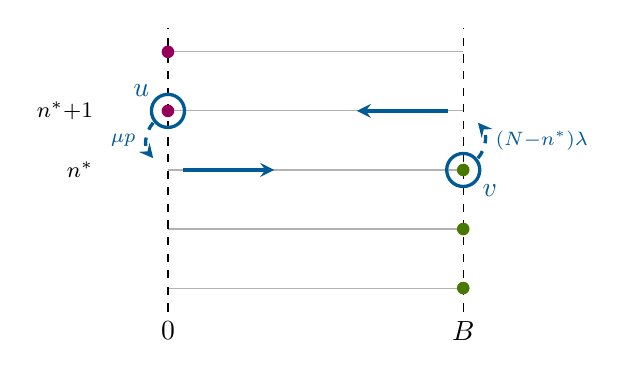
\begin{tikzpicture}[scale=0.75]
				\foreach \y in {0,1,2,3,4}{ \draw[gray!60] (0,\y) -- (5,\y); }
				\draw[dashed] (0,-0.4) node[below] {$0$} -- (0,4.4);
				\draw[dashed] (5,-0.4) node[below] {$B$} -- (5,4.4);
				\node[anchor=east] at (-1.1,2) {\footnotesize $\ns$};
				\node[anchor=east] at (-1.1,3) {\footnotesize $\ns{+}1$};
				% atoms
				\foreach \y in {0,1,2}{ \node[verdecito!80!black, fill=verdecito!80!black, circle, minimum size=.16cm, inner sep=0pt] at (5,\y) {}; }
				\foreach \y in {3,4}{ \node[rojito, fill=rojito, circle, minimum size=.16cm, inner sep=0pt] at (0,\y) {}; }
				% gateways
				\node[draw, very thick, azulcito, circle, minimum size=.42cm] at (5,2) {};
				\node[draw, very thick, azulcito, circle, minimum size=.42cm] at (0,3) {};
				\node[azulcito] at (5.45,1.65) {$v$};
				\node[azulcito] at (-0.45,3.35) {$u$};
				\draw[->, very thick, azulcito, dashed] (5.25,2.2) to[bend right=40] node[right] {\scriptsize $(N{-}\ns)\lambda$} (5.25,2.8);
				\draw[->, very thick, azulcito] (4.75,3) -- (3.2,3);
				\draw[->, very thick, azulcito, dashed] (-0.25,2.8) to[bend right=40] node[left] {\scriptsize $\mu p$} (-0.25,2.2);
				\draw[->, very thick, azulcito] (0.25,2) -- (1.8,2);
			\end{tikzpicture}
			\end{center}
		\end{column}
	\end{columns}
\end{frame}

\begin{frame}{Proof, part 1: positive boundary data, positive interior}

	\begin{myitem}
		\item Fix gateway data $(u,v)\geq 0$, not both zero.
		\item<2-> Solve the interior system $\mathbf{f}'R=\mathbf{f}Q$, with each mode's condition at its \alert{inflow} end.
		\item<3-> The solution is \alert{positive} on $(0,B)$: a \alert{maximum principle}, which again rests on \alert{reversibility}.
	\end{myitem}

	\vfill
	\uncover<4->{
	\begin{block}{}
		\begin{center}
		Positive boundary data $\Rightarrow$ positive interior.\\
		It remains to find the boundary data.
		\end{center}
	\end{block}
	}
\end{frame}

\begin{frame}{Proof, part 2: the gateways}

	\begin{myitem}
		\item Feeding the interior back to the boundaries: $(u',v') = T(u,v)$, with $T$ a $2\times 2$ matrix, \alert{$T>0$} by part 1.
		\item A stationary law needs a fixed point: $T(u,v)=(u,v)$.
		\item<2-> \alert{Flow conservation}: what leaves the boundaries through the gateways comes back. Testing the balance equations with $\psi\equiv 1$:
		\begin{equation*}
			w^\top T = w^\top, \qquad w = \big(\mu p,\ (N-\ns)\lambda\big) > 0 .
		\end{equation*}
		\item<3-> \alert{Perron--Frobenius}: a positive left eigenvector with eigenvalue $1$ makes $1$ the spectral radius of $T$, \alert{simple}, with a \alert{positive} right eigenvector $(u,v)$, unique up to scale.
	\end{myitem}
\end{frame}

\begin{frame}{Proof, part 2: the other atoms}

	\begin{myitem}
		\item With the gateways known, the remaining atoms solve a \alert{birth--death recursion} on each side:
		\begin{itemize}
			\item at $x=B$, on $\{0,\ldots,\ns\}$, starting from $v$;
			\item at $x=0$, on $\{\ns+1,\ldots,N\}$, starting from $u$.
		\end{itemize}
		\item<2-> The inputs from the interior are positive, so \alert{every atom is positive}.
		\item<3-> Normalise. Uniqueness comes from the simplicity of the Perron eigenvalue. \hfill $\square$
	\end{myitem}
\end{frame}

\begin{frame}{Work in progress: feedback fluid queues}

	\begin{myitem}
		\item We are exploring the connection with \alert{feedback fluid queues} \cite{MMS2003}, where the sources' rates depend on the buffer.
		\item<2-> There, excursions away from the empty buffer are \alert{unaffected} by the feedback.
		\item<3-> If this carries over, the whole effect of the throttle reduces to \alert{one number}: the mass at the empty bucket.
	\end{myitem}
\end{frame}

%=====================================================================
\section{Fluid limit}
%=====================================================================

\begin{frame}{The two costs}

	\begin{columns}[T]
		\begin{column}{0.5\textwidth}
			\begin{block}{Throttling}
				\begin{equation*}
					P_{\rm thr} = \sum_{n>\ns} \pi^0_n
				\end{equation*}
				fraction of time the fleet is held to $p$.
			\end{block}
		\end{column}
		\begin{column}{0.5\textwidth}
			\begin{block}{Waste}
				\begin{equation*}
					W = \sum_{n\leq\ns} (p-nc)\,\pi^B_n
				\end{equation*}
				refill discarded at the cap.
			\end{block}
		\end{column}
	\end{columns}

\end{frame}

\begin{frame}{Fluid scaling}

	Scale the plan with the fleet:
	\begin{equation*}
		p = N\bar p, \qquad B = N\bar b .
	\end{equation*}

	\vfill
	\pause

	Fluid variables:
	\begin{equation*}
		\bar n(t) = \frac{n(t)}{N}\ \ \text{(fraction of agents active)}, \qquad \bar x(t) = \frac{x(t)}{N}\ \ \text{(tokens left, per agent)}.
	\end{equation*}
\end{frame}

\begin{frame}{The fluid equations}

	\begin{myitem}
		\item \alert{Interior}, $0<\bar x<\bar b$:
		\begin{equation*}
			\dot{\bar n} = \lambda(1-\bar n) - \nu\,\bar n, \qquad \dot{\bar x} = \bar p - c\,\bar n .
		\end{equation*}
		\item<2-> \alert{Full bucket}, $\bar x=\bar b$ and $c\bar n<\bar p$: $\ \dot{\bar x}=0$, and $\bar n$ as in the interior.
		\item<3-> \alert{Empty bucket}, $\bar x=0$ and $c\bar n>\bar p$: $\ \dot{\bar x}=0$, and the fleet is \alert{throttled}:
		\begin{equation*}
			\dot{\bar n} = \lambda(1-\bar n) - \nu\,\frac{\bar p}{c} .
		\end{equation*}
	\end{myitem}
\end{frame}

\begin{frame}{Convergence}{Work in progress}

	\begin{myitem}
		\item Expected: $\big(n(t)/N,\ x(t)/N\big) \to \big(\bar n(t),\bar x(t)\big)$ on compact time intervals, as $N\to\infty$.
		\item<2-> In the interior, a \alert{density-dependent} jump process \cite{Kurtz1970,EthierKurtz1986}.
		\item<3-> At the boundaries the vector field is discontinuous: the limit \alert{slides} along them.
	\end{myitem}

	\vfill
	\uncover<4->{
	\begin{block}{}
		No formal proof yet; it should follow from standard arguments for density-dependent processes in the Kurtz setting.
	\end{block}
	}
\end{frame}

\begin{frame}{Phase portrait: over-provisioned}

	\begin{columns}
		\begin{column}{0.5\textwidth}
			\begin{center}
			%% Fluid phase portrait (x horizontal, n vertical, as in the state-space picture)
%% lambda=1.0, nu=3.0, c=1.0, rho=0.250, pbar=0.36, bbar=0.2; generated by scripts/phase_portraits.py
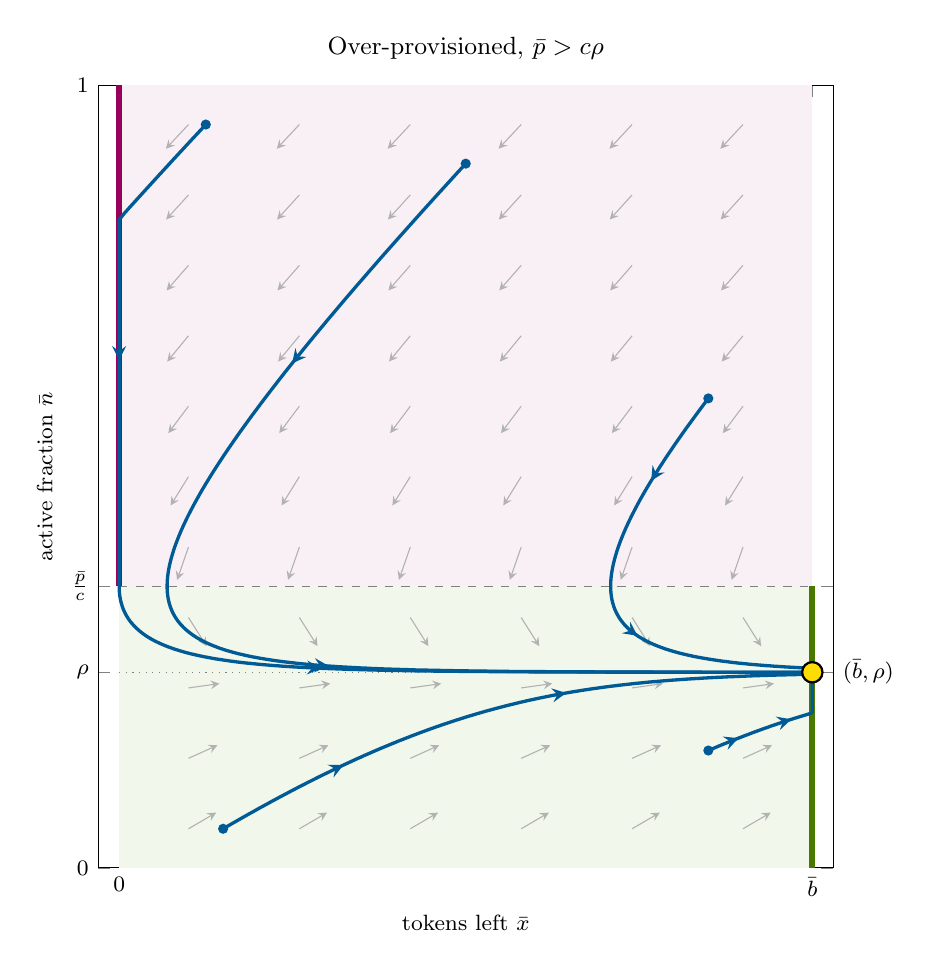
\begin{tikzpicture}
\begin{axis}[width=0.9\textwidth, height=0.95\textwidth, xmin=-0.006, xmax=0.20600000000000002, ymin=0, ymax=1,
  axis lines=box, xlabel={tokens left $\bar x$}, ylabel={active fraction $\bar n$},
  xtick={0,0.2}, xticklabels={0,$\bar b$},
  ytick={0,0.25,0.36,1}, yticklabels={0,$\rho$,$\frac{\bar p}{c}$,1},
  title={Over-provisioned, $\bar p > c\rho$}, title style={font=\small},
  tick label style={font=\footnotesize}, label style={font=\footnotesize}, clip=false]
% regions: filling (below pbar/c) and draining (above)
\fill[verdecito!8] (axis cs:0,0) rectangle (axis cs:0.2,0.36);
\fill[rojito!6] (axis cs:0,0.36) rectangle (axis cs:0.2,1);
\draw[dashed, gray] (axis cs:0,0.36) -- (axis cs:0.2,0.36);
\draw[dotted, gray] (axis cs:0,0.25) -- (axis cs:0.2,0.25);
% sticky boundaries: full on the right (filling modes), empty on the left (draining modes)
\draw[line width=2.2pt, verdecito!80!black] (axis cs:0.2,0) -- (axis cs:0.2,0.36);
\draw[line width=2.2pt, rojito] (axis cs:0,0.36) -- (axis cs:0,1);
% vector field
\addplot[gray!60, -stealth, quiver={u=\thisrowno{2}, v=\thisrowno{3}}] table[row sep=newline] {
0.0200 0.0500 0.007998 0.02064
0.0520 0.0500 0.007998 0.02064
0.0840 0.0500 0.007998 0.02064
0.1160 0.0500 0.007998 0.02064
0.1480 0.0500 0.007998 0.02064
0.1800 0.0500 0.007998 0.02064
0.0200 0.1400 0.008356 0.01671
0.0520 0.1400 0.008356 0.01671
0.0840 0.1400 0.008356 0.01671
0.1160 0.1400 0.008356 0.01671
0.1480 0.1400 0.008356 0.01671
0.1800 0.1400 0.008356 0.01671
0.0200 0.2300 0.008933 0.00550
0.0520 0.2300 0.008933 0.00550
0.0840 0.2300 0.008933 0.00550
0.1160 0.2300 0.008933 0.00550
0.1480 0.2300 0.008933 0.00550
0.1800 0.2300 0.008933 0.00550
0.0200 0.3200 0.005231 -0.03662
0.0520 0.3200 0.005231 -0.03662
0.0840 0.3200 0.005231 -0.03662
0.1160 0.3200 0.005231 -0.03662
0.1480 0.3200 0.005231 -0.03662
0.1800 0.3200 0.005231 -0.03662
0.0200 0.4100 -0.003275 -0.04192
0.0520 0.4100 -0.003275 -0.04192
0.0840 0.4100 -0.003275 -0.04192
0.1160 0.4100 -0.003275 -0.04192
0.1480 0.4100 -0.003275 -0.04192
0.1800 0.4100 -0.003275 -0.04192
0.0200 0.5000 -0.005161 -0.03687
0.0520 0.5000 -0.005161 -0.03687
0.0840 0.5000 -0.005161 -0.03687
0.1160 0.5000 -0.005161 -0.03687
0.1480 0.5000 -0.005161 -0.03687
0.1800 0.5000 -0.005161 -0.03687
0.0200 0.5900 -0.005811 -0.03436
0.0520 0.5900 -0.005811 -0.03436
0.0840 0.5900 -0.005811 -0.03436
0.1160 0.5900 -0.005811 -0.03436
0.1480 0.5900 -0.005811 -0.03436
0.1800 0.5900 -0.005811 -0.03436
0.0200 0.6800 -0.006130 -0.03295
0.0520 0.6800 -0.006130 -0.03295
0.0840 0.6800 -0.006130 -0.03295
0.1160 0.6800 -0.006130 -0.03295
0.1480 0.6800 -0.006130 -0.03295
0.1800 0.6800 -0.006130 -0.03295
0.0200 0.7700 -0.006318 -0.03205
0.0520 0.7700 -0.006318 -0.03205
0.0840 0.7700 -0.006318 -0.03205
0.1160 0.7700 -0.006318 -0.03205
0.1480 0.7700 -0.006318 -0.03205
0.1800 0.7700 -0.006318 -0.03205
0.0200 0.8600 -0.006441 -0.03143
0.0520 0.8600 -0.006441 -0.03143
0.0840 0.8600 -0.006441 -0.03143
0.1160 0.8600 -0.006441 -0.03143
0.1480 0.8600 -0.006441 -0.03143
0.1800 0.8600 -0.006441 -0.03143
0.0200 0.9500 -0.006528 -0.03098
0.0520 0.9500 -0.006528 -0.03098
0.0840 0.9500 -0.006528 -0.03098
0.1160 0.9500 -0.006528 -0.03098
0.1480 0.9500 -0.006528 -0.03098
0.1800 0.9500 -0.006528 -0.03098
};
\addplot[azulcito, very thick, postaction={decorate}, decoration={markings, mark=at position 0.22 with {\arrow{stealth}}, mark=at position 0.6 with {\arrow{stealth}}}] coordinates {(0.10000,0.9000) (0.09775,0.8892) (0.09566,0.8790) (0.09360,0.8690) (0.09158,0.8592) (0.08960,0.8495) (0.08766,0.8400) (0.08576,0.8306) (0.08390,0.8214) (0.08207,0.8123) (0.08028,0.8034) (0.07852,0.7946) (0.07680,0.7860) (0.07511,0.7775) (0.07346,0.7691) (0.07183,0.7608) (0.07025,0.7527) (0.06869,0.7448) (0.06717,0.7369) (0.06567,0.7292) (0.06421,0.7216) (0.06278,0.7141) (0.06138,0.7067) (0.06000,0.6995) (0.05866,0.6923) (0.05734,0.6853) (0.05606,0.6784) (0.05480,0.6716) (0.05356,0.6649) (0.05236,0.6583) (0.05117,0.6518) (0.05002,0.6454) (0.04889,0.6392) (0.04778,0.6330) (0.04670,0.6269) (0.04565,0.6209) (0.04462,0.6150) (0.04361,0.6092) (0.04262,0.6035) (0.04166,0.5979) (0.04072,0.5924) (0.03980,0.5869) (0.03890,0.5816) (0.03802,0.5763) (0.03717,0.5711) (0.03633,0.5660) (0.03552,0.5610) (0.03472,0.5561) (0.03395,0.5512) (0.03319,0.5464) (0.03246,0.5417) (0.03174,0.5371) (0.03104,0.5325) (0.03036,0.5281) (0.02969,0.5236) (0.02905,0.5193) (0.02842,0.5150) (0.02781,0.5108) (0.02721,0.5067) (0.02663,0.5026) (0.02607,0.4986) (0.02552,0.4946) (0.02499,0.4908) (0.02447,0.4869) (0.02397,0.4832) (0.02349,0.4795) (0.02302,0.4758) (0.02256,0.4722) (0.02212,0.4687) (0.02169,0.4652) (0.02128,0.4618) (0.02088,0.4585) (0.02049,0.4551) (0.02011,0.4519) (0.01975,0.4487) (0.01940,0.4455) (0.01907,0.4424) (0.01874,0.4394) (0.01843,0.4364) (0.01813,0.4334) (0.01784,0.4305) (0.01757,0.4276) (0.01730,0.4248) (0.01705,0.4220) (0.01657,0.4166) (0.01614,0.4114) (0.01575,0.4063) (0.01540,0.4013) (0.01509,0.3966) (0.01481,0.3920) (0.01457,0.3875) (0.01437,0.3832) (0.01420,0.3790) (0.01407,0.3749) (0.01396,0.3710) (0.01389,0.3672) (0.01384,0.3617) (0.01385,0.3564) (0.01392,0.3514) (0.01405,0.3467) (0.01424,0.3421) (0.01448,0.3378) (0.01477,0.3337) (0.01511,0.3298) (0.01549,0.3260) (0.01592,0.3225) (0.01639,0.3191) (0.01690,0.3158) (0.01745,0.3128) (0.01804,0.3098) (0.01865,0.3070) (0.01931,0.3043) (0.01999,0.3018) (0.02070,0.2994) (0.02119,0.2978) (0.02170,0.2963) (0.02221,0.2948) (0.02274,0.2934) (0.02328,0.2921) (0.02383,0.2907) (0.02438,0.2895) (0.02495,0.2882) (0.02553,0.2870) (0.02612,0.2858) (0.02672,0.2847) (0.02733,0.2836) (0.02794,0.2826) (0.02856,0.2815) (0.02920,0.2805) (0.02984,0.2796) (0.03048,0.2786) (0.03114,0.2777) (0.03180,0.2769) (0.03247,0.2760) (0.03314,0.2752) (0.03382,0.2744) (0.03451,0.2736) (0.03521,0.2729) (0.03590,0.2722) (0.03661,0.2715) (0.03732,0.2708) (0.03804,0.2701) (0.03876,0.2695) (0.03949,0.2689) (0.04022,0.2683) (0.04095,0.2677) (0.04169,0.2672) (0.04244,0.2666) (0.04319,0.2661) (0.04394,0.2656) (0.04470,0.2651) (0.04546,0.2646) (0.04622,0.2642) (0.04699,0.2637) (0.04776,0.2633) (0.04854,0.2629) (0.04932,0.2625) (0.05010,0.2621) (0.05088,0.2617) (0.05167,0.2613) (0.05246,0.2610) (0.05326,0.2606) (0.05405,0.2603) (0.05485,0.2600) (0.05565,0.2596) (0.05646,0.2593) (0.05726,0.2590) (0.05807,0.2588) (0.05888,0.2585) (0.05970,0.2582) (0.06051,0.2580) (0.06133,0.2577) (0.06215,0.2575) (0.06297,0.2572) (0.06379,0.2570) (0.06462,0.2568) (0.06544,0.2566) (0.06627,0.2564) (0.06710,0.2562) (0.06793,0.2560) (0.06877,0.2558) (0.06960,0.2556) (0.07044,0.2554) (0.07127,0.2553) (0.07211,0.2551) (0.07295,0.2549) (0.07379,0.2548) (0.07464,0.2546) (0.07548,0.2545) (0.07633,0.2543) (0.07717,0.2542) (0.07802,0.2541) (0.07887,0.2539) (0.07971,0.2538) (0.08056,0.2537) (0.08142,0.2536) (0.08227,0.2535) (0.08312,0.2534) (0.08397,0.2532) (0.08483,0.2531) (0.08568,0.2530) (0.08654,0.2530) (0.08740,0.2529) (0.08825,0.2528) (0.08911,0.2527) (0.08997,0.2526) (0.09083,0.2525) (0.09169,0.2524) (0.09255,0.2524) (0.09341,0.2523) (0.09428,0.2522) (0.09514,0.2521) (0.09600,0.2521) (0.09686,0.2520) (0.09773,0.2519) (0.09859,0.2519) (0.09946,0.2518) (0.10032,0.2518) (0.10119,0.2517) (0.10206,0.2517) (0.10292,0.2516) (0.10379,0.2516) (0.10466,0.2515) (0.10553,0.2515) (0.10640,0.2514) (0.10726,0.2514) (0.10813,0.2513) (0.10900,0.2513) (0.10987,0.2512) (0.11074,0.2512) (0.11161,0.2512) (0.11248,0.2511) (0.11336,0.2511) (0.11423,0.2511) (0.11510,0.2510) (0.11597,0.2510) (0.11684,0.2510) (0.11771,0.2509) (0.11859,0.2509) (0.11946,0.2509) (0.12033,0.2508) (0.12121,0.2508) (0.12208,0.2508) (0.12295,0.2508) (0.12383,0.2507) (0.12470,0.2507) (0.12558,0.2507) (0.12645,0.2507) (0.12733,0.2507) (0.12820,0.2506) (0.12908,0.2506) (0.12995,0.2506) (0.13083,0.2506) (0.13170,0.2506) (0.13258,0.2505) (0.13345,0.2505) (0.13433,0.2505) (0.13520,0.2505) (0.13608,0.2505) (0.13696,0.2505) (0.13783,0.2504) (0.13871,0.2504) (0.13959,0.2504) (0.14046,0.2504) (0.14134,0.2504) (0.14222,0.2504) (0.14309,0.2504) (0.14397,0.2504) (0.14485,0.2503) (0.14573,0.2503) (0.14660,0.2503) (0.14748,0.2503) (0.14836,0.2503) (0.14924,0.2503) (0.15011,0.2503) (0.15099,0.2503) (0.15187,0.2503) (0.15275,0.2503) (0.15362,0.2503) (0.15450,0.2502) (0.15538,0.2502) (0.15626,0.2502) (0.15714,0.2502) (0.15802,0.2502) (0.15889,0.2502) (0.15977,0.2502) (0.16065,0.2502) (0.16153,0.2502) (0.16241,0.2502) (0.16329,0.2502) (0.16416,0.2502) (0.16504,0.2502) (0.16592,0.2502) (0.16680,0.2502) (0.16768,0.2502) (0.16856,0.2501) (0.16944,0.2501) (0.17032,0.2501) (0.17120,0.2501) (0.17207,0.2501) (0.17295,0.2501) (0.17383,0.2501) (0.17471,0.2501) (0.17559,0.2501) (0.17647,0.2501) (0.17735,0.2501) (0.17823,0.2501) (0.17911,0.2501) (0.17999,0.2501) (0.18087,0.2501) (0.18174,0.2501) (0.18262,0.2501) (0.18350,0.2501) (0.18438,0.2501) (0.18526,0.2501) (0.18614,0.2501) (0.18702,0.2501) (0.18790,0.2501) (0.18878,0.2501) (0.18966,0.2501) (0.19054,0.2501) (0.19142,0.2501) (0.19230,0.2501) (0.19318,0.2501) (0.19406,0.2501) (0.19494,0.2501) (0.19582,0.2501) (0.19670,0.2501) (0.19757,0.2501) (0.19845,0.2500) (0.19933,0.2500)};
\node[circle, fill=azulcito, inner sep=1.3pt] at (axis cs:0.1,0.9) {};
\addplot[azulcito, very thick, postaction={decorate}, decoration={markings, mark=at position 0.22 with {\arrow{stealth}}, mark=at position 0.6 with {\arrow{stealth}}}] coordinates {(0.17000,0.6000) (0.16900,0.5942) (0.16808,0.5887) (0.16717,0.5833) (0.16629,0.5780) (0.16543,0.5728) (0.16459,0.5677) (0.16376,0.5627) (0.16296,0.5577) (0.16218,0.5528) (0.16142,0.5480) (0.16068,0.5433) (0.15995,0.5386) (0.15925,0.5340) (0.15856,0.5295) (0.15789,0.5251) (0.15724,0.5207) (0.15660,0.5164) (0.15599,0.5122) (0.15539,0.5080) (0.15480,0.5039) (0.15423,0.4999) (0.15368,0.4959) (0.15314,0.4920) (0.15262,0.4882) (0.15212,0.4844) (0.15163,0.4807) (0.15115,0.4770) (0.15069,0.4734) (0.15024,0.4699) (0.14981,0.4664) (0.14939,0.4629) (0.14899,0.4595) (0.14860,0.4562) (0.14822,0.4529) (0.14785,0.4497) (0.14750,0.4465) (0.14716,0.4434) (0.14683,0.4404) (0.14652,0.4373) (0.14621,0.4344) (0.14592,0.4314) (0.14564,0.4285) (0.14537,0.4257) (0.14511,0.4229) (0.14463,0.4175) (0.14419,0.4122) (0.14379,0.4071) (0.14344,0.4021) (0.14312,0.3973) (0.14284,0.3927) (0.14259,0.3882) (0.14239,0.3839) (0.14221,0.3796) (0.14207,0.3756) (0.14196,0.3716) (0.14188,0.3678) (0.14182,0.3622) (0.14183,0.3570) (0.14189,0.3520) (0.14202,0.3472) (0.14220,0.3426) (0.14243,0.3383) (0.14272,0.3341) (0.14305,0.3302) (0.14343,0.3264) (0.14386,0.3229) (0.14432,0.3194) (0.14483,0.3162) (0.14537,0.3131) (0.14595,0.3101) (0.14657,0.3073) (0.14722,0.3046) (0.14790,0.3021) (0.14861,0.2996) (0.14910,0.2981) (0.14960,0.2965) (0.15011,0.2951) (0.15064,0.2937) (0.15117,0.2923) (0.15172,0.2909) (0.15228,0.2897) (0.15284,0.2884) (0.15342,0.2872) (0.15401,0.2860) (0.15460,0.2849) (0.15521,0.2838) (0.15582,0.2827) (0.15645,0.2817) (0.15708,0.2807) (0.15771,0.2797) (0.15836,0.2788) (0.15901,0.2779) (0.15967,0.2770) (0.16034,0.2762) (0.16102,0.2753) (0.16170,0.2745) (0.16238,0.2738) (0.16308,0.2730) (0.16377,0.2723) (0.16448,0.2716) (0.16519,0.2709) (0.16590,0.2702) (0.16662,0.2696) (0.16735,0.2690) (0.16808,0.2684) (0.16882,0.2678) (0.16956,0.2673) (0.17030,0.2667) (0.17105,0.2662) (0.17180,0.2657) (0.17256,0.2652) (0.17332,0.2647) (0.17408,0.2642) (0.17485,0.2638) (0.17562,0.2634) (0.17640,0.2629) (0.17717,0.2625) (0.17795,0.2621) (0.17874,0.2617) (0.17953,0.2614) (0.18032,0.2610) (0.18111,0.2607) (0.18191,0.2603) (0.18270,0.2600) (0.18351,0.2597) (0.18431,0.2594) (0.18512,0.2591) (0.18592,0.2588) (0.18673,0.2585) (0.18755,0.2583) (0.18836,0.2580) (0.18918,0.2577) (0.19000,0.2575) (0.19082,0.2573) (0.19164,0.2570) (0.19247,0.2568) (0.19329,0.2566) (0.19412,0.2564) (0.19495,0.2562) (0.19578,0.2560) (0.19661,0.2558) (0.19745,0.2556) (0.19828,0.2554) (0.19912,0.2553) (0.19996,0.2551) (0.20000,0.2513)};
\node[circle, fill=azulcito, inner sep=1.3pt] at (axis cs:0.17,0.6) {};
\addplot[azulcito, very thick, postaction={decorate}, decoration={markings, mark=at position 0.22 with {\arrow{stealth}}, mark=at position 0.6 with {\arrow{stealth}}}] coordinates {(0.03000,0.0500) (0.03130,0.0533) (0.03252,0.0565) (0.03372,0.0595) (0.03492,0.0626) (0.03610,0.0655) (0.03728,0.0685) (0.03844,0.0713) (0.03959,0.0742) (0.04072,0.0770) (0.04185,0.0797) (0.04297,0.0824) (0.04407,0.0851) (0.04517,0.0877) (0.04625,0.0903) (0.04733,0.0928) (0.04839,0.0953) (0.04944,0.0978) (0.05049,0.1002) (0.05152,0.1026) (0.05255,0.1049) (0.05356,0.1072) (0.05457,0.1095) (0.05557,0.1117) (0.05656,0.1139) (0.05754,0.1161) (0.05851,0.1182) (0.05947,0.1203) (0.06043,0.1223) (0.06137,0.1244) (0.06231,0.1264) (0.06324,0.1283) (0.06417,0.1303) (0.06508,0.1322) (0.06599,0.1340) (0.06689,0.1359) (0.06778,0.1377) (0.06867,0.1395) (0.06955,0.1412) (0.07042,0.1430) (0.07129,0.1447) (0.07214,0.1463) (0.07299,0.1480) (0.07384,0.1496) (0.07468,0.1512) (0.07551,0.1528) (0.07634,0.1543) (0.07716,0.1558) (0.07797,0.1573) (0.07878,0.1588) (0.07958,0.1602) (0.08038,0.1617) (0.08117,0.1631) (0.08195,0.1644) (0.08273,0.1658) (0.08351,0.1671) (0.08428,0.1685) (0.08504,0.1697) (0.08580,0.1710) (0.08655,0.1723) (0.08730,0.1735) (0.08804,0.1747) (0.08878,0.1759) (0.08952,0.1771) (0.09025,0.1783) (0.09097,0.1794) (0.09169,0.1805) (0.09241,0.1816) (0.09312,0.1827) (0.09383,0.1838) (0.09453,0.1848) (0.09523,0.1859) (0.09592,0.1869) (0.09661,0.1879) (0.09730,0.1889) (0.09798,0.1898) (0.09866,0.1908) (0.09934,0.1917) (0.10001,0.1927) (0.10067,0.1936) (0.10134,0.1945) (0.10200,0.1953) (0.10266,0.1962) (0.10331,0.1971) (0.10396,0.1979) (0.10461,0.1987) (0.10525,0.1996) (0.10589,0.2004) (0.10716,0.2019) (0.10842,0.2034) (0.10967,0.2049) (0.11090,0.2063) (0.11213,0.2077) (0.11334,0.2090) (0.11454,0.2103) (0.11573,0.2116) (0.11692,0.2128) (0.11809,0.2140) (0.11925,0.2151) (0.12041,0.2162) (0.12156,0.2173) (0.12269,0.2183) (0.12382,0.2193) (0.12495,0.2203) (0.12606,0.2212) (0.12717,0.2221) (0.12827,0.2230) (0.12936,0.2238) (0.13045,0.2247) (0.13152,0.2255) (0.13260,0.2262) (0.13367,0.2270) (0.13473,0.2277) (0.13578,0.2284) (0.13683,0.2291) (0.13788,0.2297) (0.13892,0.2304) (0.13995,0.2310) (0.14098,0.2316) (0.14201,0.2322) (0.14303,0.2327) (0.14404,0.2333) (0.14505,0.2338) (0.14606,0.2343) (0.14707,0.2348) (0.14806,0.2353) (0.14906,0.2358) (0.15005,0.2362) (0.15104,0.2366) (0.15203,0.2371) (0.15301,0.2375) (0.15399,0.2379) (0.15496,0.2382) (0.15594,0.2386) (0.15691,0.2390) (0.15787,0.2393) (0.15884,0.2397) (0.15980,0.2400) (0.16076,0.2403) (0.16171,0.2406) (0.16267,0.2409) (0.16362,0.2412) (0.16457,0.2415) (0.16552,0.2417) (0.16646,0.2420) (0.16740,0.2422) (0.16834,0.2425) (0.16928,0.2427) (0.17022,0.2430) (0.17116,0.2432) (0.17209,0.2434) (0.17302,0.2436) (0.17395,0.2438) (0.17488,0.2440) (0.17581,0.2442) (0.17673,0.2444) (0.17766,0.2445) (0.17858,0.2447) (0.17950,0.2449) (0.18042,0.2450) (0.18134,0.2452) (0.18226,0.2454) (0.18318,0.2455) (0.18409,0.2456) (0.18501,0.2458) (0.18592,0.2459) (0.18683,0.2460) (0.18774,0.2462) (0.18865,0.2463) (0.18956,0.2464) (0.19047,0.2465) (0.19138,0.2466) (0.19229,0.2467) (0.19319,0.2468) (0.19410,0.2469) (0.19500,0.2470) (0.19590,0.2471) (0.19681,0.2472) (0.19771,0.2473) (0.19861,0.2474) (0.19951,0.2475) (0.20000,0.2490)};
\node[circle, fill=azulcito, inner sep=1.3pt] at (axis cs:0.03,0.05) {};
\addplot[azulcito, very thick, postaction={decorate}, decoration={markings, mark=at position 0.22 with {\arrow{stealth}}, mark=at position 0.6 with {\arrow{stealth}}}] coordinates {(0.17000,0.1500) (0.17088,0.1517) (0.17171,0.1532) (0.17253,0.1548) (0.17335,0.1563) (0.17416,0.1578) (0.17497,0.1592) (0.17577,0.1607) (0.17656,0.1621) (0.17735,0.1635) (0.17814,0.1649) (0.17891,0.1662) (0.17969,0.1675) (0.18045,0.1689) (0.18122,0.1701) (0.18197,0.1714) (0.18273,0.1727) (0.18347,0.1739) (0.18422,0.1751) (0.18495,0.1763) (0.18569,0.1775) (0.18641,0.1786) (0.18714,0.1797) (0.18786,0.1809) (0.18857,0.1820) (0.18928,0.1830) (0.18999,0.1841) (0.19069,0.1851) (0.19139,0.1862) (0.19208,0.1872) (0.19277,0.1882) (0.19345,0.1892) (0.19413,0.1901) (0.19481,0.1911) (0.19549,0.1920) (0.19616,0.1929) (0.19682,0.1938) (0.19749,0.1947) (0.19815,0.1956) (0.19880,0.1965) (0.19945,0.1973) (0.20000,0.1990) (0.20000,0.2037) (0.20000,0.2079) (0.20000,0.2124) (0.20000,0.2169) (0.20000,0.2213) (0.20000,0.2256) (0.20000,0.2298) (0.20000,0.2339) (0.20000,0.2379) (0.20000,0.2420) (0.20000,0.2461)};
\node[circle, fill=azulcito, inner sep=1.3pt] at (axis cs:0.17,0.15) {};
\addplot[azulcito, very thick, postaction={decorate}, decoration={markings, mark=at position 0.22 with {\arrow{stealth}}, mark=at position 0.6 with {\arrow{stealth}}}] coordinates {(0.02500,0.9500) (0.02255,0.9383) (0.02025,0.9274) (0.01800,0.9166) (0.01580,0.9061) (0.01363,0.8956) (0.01151,0.8854) (0.00943,0.8753) (0.00739,0.8654) (0.00538,0.8556) (0.00342,0.8460) (0.00149,0.8365) (0.00000,0.8283) (0.00000,0.8211) (0.00000,0.8139) (0.00000,0.8068) (0.00000,0.7997) (0.00000,0.7927) (0.00000,0.7858) (0.00000,0.7789) (0.00000,0.7720) (0.00000,0.7652) (0.00000,0.7585) (0.00000,0.7518) (0.00000,0.7452) (0.00000,0.7386) (0.00000,0.7321) (0.00000,0.7256) (0.00000,0.7192) (0.00000,0.7128) (0.00000,0.7065) (0.00000,0.7002) (0.00000,0.6940) (0.00000,0.6878) (0.00000,0.6817) (0.00000,0.6757) (0.00000,0.6696) (0.00000,0.6637) (0.00000,0.6577) (0.00000,0.6519) (0.00000,0.6460) (0.00000,0.6402) (0.00000,0.6345) (0.00000,0.6288) (0.00000,0.6232) (0.00000,0.6176) (0.00000,0.6120) (0.00000,0.6065) (0.00000,0.6010) (0.00000,0.5956) (0.00000,0.5902) (0.00000,0.5849) (0.00000,0.5796) (0.00000,0.5743) (0.00000,0.5691) (0.00000,0.5639) (0.00000,0.5588) (0.00000,0.5537) (0.00000,0.5486) (0.00000,0.5436) (0.00000,0.5387) (0.00000,0.5337) (0.00000,0.5288) (0.00000,0.5240) (0.00000,0.5192) (0.00000,0.5144) (0.00000,0.5097) (0.00000,0.5050) (0.00000,0.5003) (0.00000,0.4957) (0.00000,0.4911) (0.00000,0.4865) (0.00000,0.4820) (0.00000,0.4776) (0.00000,0.4731) (0.00000,0.4687) (0.00000,0.4643) (0.00000,0.4600) (0.00000,0.4557) (0.00000,0.4514) (0.00000,0.4472) (0.00000,0.4430) (0.00000,0.4388) (0.00000,0.4347) (0.00000,0.4306) (0.00000,0.4265) (0.00000,0.4225) (0.00000,0.4185) (0.00000,0.4125) (0.00000,0.4067) (0.00000,0.4008) (0.00000,0.3951) (0.00000,0.3894) (0.00000,0.3838) (0.00000,0.3783) (0.00000,0.3728) (0.00000,0.3674) (0.00000,0.3621) (0.00001,0.3569) (0.00008,0.3518) (0.00020,0.3471) (0.00039,0.3425) (0.00062,0.3382) (0.00091,0.3341) (0.00124,0.3301) (0.00162,0.3264) (0.00205,0.3228) (0.00252,0.3194) (0.00302,0.3161) (0.00357,0.3130) (0.00415,0.3101) (0.00477,0.3072) (0.00542,0.3046) (0.00610,0.3020) (0.00681,0.2996) (0.00730,0.2980) (0.00780,0.2965) (0.00831,0.2950) (0.00884,0.2936) (0.00937,0.2922) (0.00992,0.2909) (0.01048,0.2896) (0.01105,0.2884) (0.01162,0.2872) (0.01221,0.2860) (0.01281,0.2849) (0.01341,0.2838) (0.01403,0.2827) (0.01465,0.2817) (0.01528,0.2807) (0.01592,0.2797) (0.01657,0.2788) (0.01722,0.2779) (0.01788,0.2770) (0.01855,0.2761) (0.01922,0.2753) (0.01990,0.2745) (0.02059,0.2737) (0.02128,0.2730) (0.02198,0.2723) (0.02269,0.2716) (0.02340,0.2709) (0.02411,0.2702) (0.02483,0.2696) (0.02556,0.2690) (0.02629,0.2684) (0.02702,0.2678) (0.02776,0.2672) (0.02851,0.2667) (0.02926,0.2662) (0.03001,0.2657) (0.03077,0.2652) (0.03153,0.2647) (0.03229,0.2642) (0.03306,0.2638) (0.03383,0.2633) (0.03461,0.2629) (0.03538,0.2625) (0.03617,0.2621) (0.03695,0.2617) (0.03774,0.2614) (0.03853,0.2610) (0.03932,0.2607) (0.04012,0.2603) (0.04092,0.2600) (0.04172,0.2597) (0.04252,0.2594) (0.04333,0.2591) (0.04414,0.2588) (0.04495,0.2585) (0.04576,0.2583) (0.04657,0.2580) (0.04739,0.2577) (0.04821,0.2575) (0.04903,0.2573) (0.04985,0.2570) (0.05068,0.2568) (0.05151,0.2566) (0.05233,0.2564) (0.05316,0.2562) (0.05399,0.2560) (0.05483,0.2558) (0.05566,0.2556) (0.05650,0.2554) (0.05733,0.2553) (0.05817,0.2551) (0.05901,0.2549) (0.05985,0.2548) (0.06070,0.2546) (0.06154,0.2545) (0.06238,0.2544) (0.06323,0.2542) (0.06408,0.2541) (0.06492,0.2540) (0.06577,0.2538) (0.06662,0.2537) (0.06747,0.2536) (0.06833,0.2535) (0.06918,0.2534) (0.07003,0.2533) (0.07089,0.2532) (0.07174,0.2531) (0.07260,0.2530) (0.07345,0.2529) (0.07431,0.2528) (0.07517,0.2527) (0.07603,0.2526) (0.07689,0.2525) (0.07775,0.2524) (0.07861,0.2524) (0.07947,0.2523) (0.08033,0.2522) (0.08119,0.2522) (0.08206,0.2521) (0.08292,0.2520) (0.08378,0.2520) (0.08465,0.2519) (0.08551,0.2518) (0.08638,0.2518) (0.08725,0.2517) (0.08811,0.2517) (0.08898,0.2516) (0.08985,0.2516) (0.09071,0.2515) (0.09158,0.2515) (0.09245,0.2514) (0.09332,0.2514) (0.09419,0.2513) (0.09506,0.2513) (0.09593,0.2512) (0.09680,0.2512) (0.09767,0.2512) (0.09854,0.2511) (0.09941,0.2511) (0.10028,0.2511) (0.10115,0.2510) (0.10203,0.2510) (0.10290,0.2510) (0.10377,0.2509) (0.10464,0.2509) (0.10552,0.2509) (0.10639,0.2509) (0.10726,0.2508) (0.10814,0.2508) (0.10901,0.2508) (0.10988,0.2507) (0.11076,0.2507) (0.11163,0.2507) (0.11251,0.2507) (0.11338,0.2507) (0.11426,0.2506) (0.11513,0.2506) (0.11601,0.2506) (0.11688,0.2506) (0.11776,0.2506) (0.11863,0.2505) (0.11951,0.2505) (0.12038,0.2505) (0.12126,0.2505) (0.12214,0.2505) (0.12301,0.2505) (0.12389,0.2504) (0.12476,0.2504) (0.12564,0.2504) (0.12652,0.2504) (0.12739,0.2504) (0.12827,0.2504) (0.12915,0.2504) (0.13003,0.2504) (0.13090,0.2503) (0.13178,0.2503) (0.13266,0.2503) (0.13353,0.2503) (0.13441,0.2503) (0.13529,0.2503) (0.13617,0.2503) (0.13705,0.2503) (0.13792,0.2503) (0.13880,0.2503) (0.13968,0.2503) (0.14056,0.2502) (0.14144,0.2502) (0.14231,0.2502) (0.14319,0.2502) (0.14407,0.2502) (0.14495,0.2502) (0.14583,0.2502) (0.14670,0.2502) (0.14758,0.2502) (0.14846,0.2502) (0.14934,0.2502) (0.15022,0.2502) (0.15110,0.2502) (0.15198,0.2502) (0.15286,0.2502) (0.15373,0.2502) (0.15461,0.2501) (0.15549,0.2501) (0.15637,0.2501) (0.15725,0.2501) (0.15813,0.2501) (0.15901,0.2501) (0.15989,0.2501) (0.16077,0.2501) (0.16164,0.2501) (0.16252,0.2501) (0.16340,0.2501) (0.16428,0.2501) (0.16516,0.2501) (0.16604,0.2501) (0.16692,0.2501) (0.16780,0.2501) (0.16868,0.2501) (0.16956,0.2501) (0.17044,0.2501) (0.17132,0.2501) (0.17220,0.2501) (0.17307,0.2501) (0.17395,0.2501) (0.17483,0.2501) (0.17571,0.2501) (0.17659,0.2501) (0.17747,0.2501) (0.17835,0.2501) (0.17923,0.2501) (0.18011,0.2501) (0.18099,0.2501) (0.18187,0.2501) (0.18275,0.2501) (0.18363,0.2501) (0.18451,0.2500) (0.18539,0.2500) (0.18627,0.2500) (0.18715,0.2500) (0.18803,0.2500) (0.18891,0.2500) (0.18979,0.2500) (0.19067,0.2500) (0.19155,0.2500) (0.19243,0.2500) (0.19331,0.2500) (0.19418,0.2500) (0.19506,0.2500) (0.19594,0.2500) (0.19682,0.2500) (0.19770,0.2500) (0.19858,0.2500) (0.19946,0.2500)};
\node[circle, fill=azulcito, inner sep=1.3pt] at (axis cs:0.025,0.95) {};
% equilibrium
\node[circle, draw=black, fill=yellow!80!orange, inner sep=2.6pt, line width=0.8pt] at (axis cs:0.2,0.25) {};
\node[font=\footnotesize, anchor=west] at (axis cs:0.20600000000000002,0.25) {$(\bar b,\rho)$};

\end{axis}
\end{tikzpicture}

			\end{center}
		\end{column}
		\begin{column}{0.5\textwidth}
			\begin{myitem}[1em]
				\item The fleet relaxes to $\rho$; the bucket \alert{fills}.
				\item Equilibrium: bucket full, $\bar n=\rho$. No throttling.
				\item Refill wasted at rate $N(\bar p - c\rho)$: of order $N$.
			\end{myitem}
			\vfill
			{\footnotesize Green edge: full bucket. Red edge: empty bucket, fleet throttled. $\lambda=1$, $\nu=3$, $c=1$.}
		\end{column}
	\end{columns}
\end{frame}

\begin{frame}{Phase portrait: under-provisioned}

	\begin{columns}
		\begin{column}{0.5\textwidth}
			\begin{center}
			%% Fluid phase portrait: lambda=1.0, nu=3.0, c=1.0, rho=0.250, pbar=0.17, bbar=0.2
%% generated by scripts/phase_portraits.py
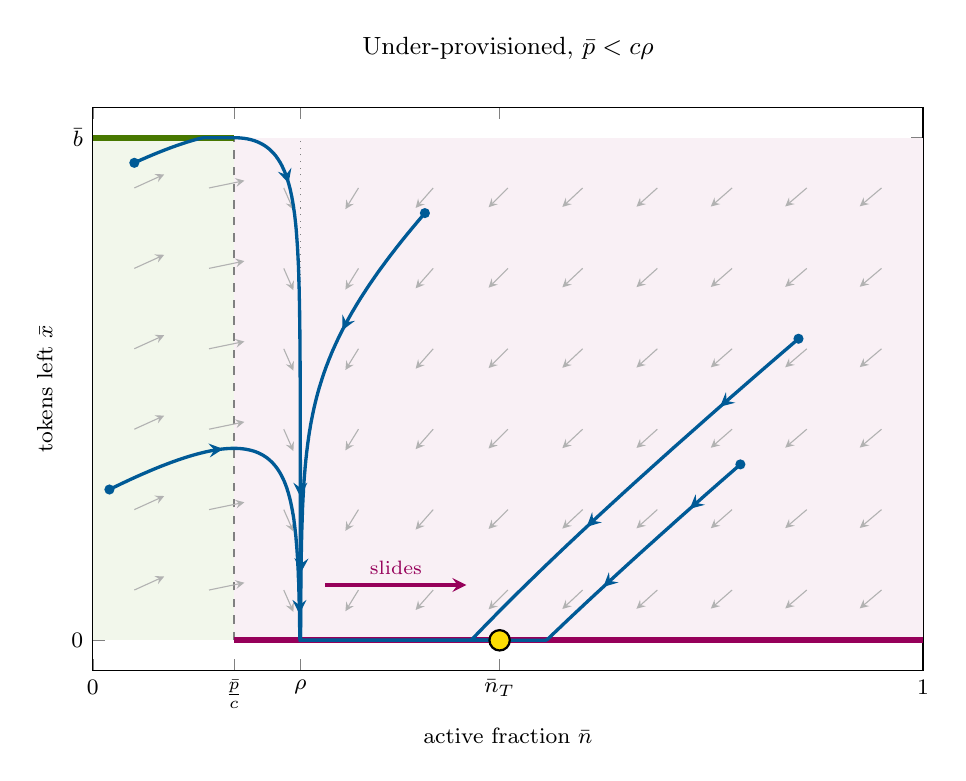
\begin{tikzpicture}
\begin{axis}[width=\textwidth, height=0.72\textwidth, xmin=0, xmax=1, ymin=-0.012, ymax=0.21200000000000002,
  axis lines=box, xlabel={active fraction $\bar n$}, ylabel={tokens left $\bar x$},
  xtick={0,0.17,0.25,0.49,1}, xticklabels={0,$\frac{\bar p}{c}$,$\rho$,$\bar n_T$,1},
  ytick={0,0.2}, yticklabels={0,$\bar b$},
  title={Under-provisioned, $\bar p < c\rho$}, title style={font=\small, yshift=8pt},
  tick label style={font=\footnotesize}, label style={font=\footnotesize}, clip=false]
% regions: filling (left of pbar/c) and draining (right)
\fill[verdecito!8] (axis cs:0,0) rectangle (axis cs:0.17,0.2);
\fill[rojito!6] (axis cs:0.17,0) rectangle (axis cs:1,0.2);
\draw[dashed, gray] (axis cs:0.17,0) -- (axis cs:0.17,0.2);
\draw[dotted, gray] (axis cs:0.25,0) -- (axis cs:0.25,0.2);
% sticky boundaries
\draw[line width=2.2pt, verdecito!80!black] (axis cs:0,0.2) -- (axis cs:0.17,0.2);
\draw[line width=2.2pt, rojito] (axis cs:0.17,0) -- (axis cs:1,0);
% vector field
\addplot[gray!60, -stealth, quiver={u=\thisrowno{2}, v=\thisrowno{3}}] table[row sep=newline] {
0.0500 0.0200 0.03600 0.005400
0.0500 0.0520 0.03600 0.005400
0.0500 0.0840 0.03600 0.005400
0.0500 0.1160 0.03600 0.005400
0.0500 0.1480 0.03600 0.005400
0.0500 0.1800 0.03600 0.005400
0.1400 0.0200 0.04259 0.002904
0.1400 0.0520 0.04259 0.002904
0.1400 0.0840 0.04259 0.002904
0.1400 0.1160 0.04259 0.002904
0.1400 0.1480 0.04259 0.002904
0.1400 0.1800 0.04259 0.002904
0.2300 0.0200 0.01159 -0.008696
0.2300 0.0520 0.01159 -0.008696
0.2300 0.0840 0.01159 -0.008696
0.2300 0.1160 0.01159 -0.008696
0.2300 0.1480 0.01159 -0.008696
0.2300 0.1800 0.01159 -0.008696
0.3200 0.0200 -0.01574 -0.008432
0.3200 0.0520 -0.01574 -0.008432
0.3200 0.0840 -0.01574 -0.008432
0.3200 0.1160 -0.01574 -0.008432
0.3200 0.1480 -0.01574 -0.008432
0.3200 0.1800 -0.01574 -0.008432
0.4100 0.0200 -0.02118 -0.007941
0.4100 0.0520 -0.02118 -0.007941
0.4100 0.0840 -0.02118 -0.007941
0.4100 0.1160 -0.02118 -0.007941
0.4100 0.1480 -0.02118 -0.007941
0.4100 0.1800 -0.02118 -0.007941
0.5000 0.0200 -0.02332 -0.007697
0.5000 0.0520 -0.02332 -0.007697
0.5000 0.0840 -0.02332 -0.007697
0.5000 0.1160 -0.02332 -0.007697
0.5000 0.1480 -0.02332 -0.007697
0.5000 0.1800 -0.02332 -0.007697
0.5900 0.0200 -0.02446 -0.007554
0.5900 0.0520 -0.02446 -0.007554
0.5900 0.0840 -0.02446 -0.007554
0.5900 0.1160 -0.02446 -0.007554
0.5900 0.1480 -0.02446 -0.007554
0.5900 0.1800 -0.02446 -0.007554
0.6800 0.0200 -0.02516 -0.007461
0.6800 0.0520 -0.02516 -0.007461
0.6800 0.0840 -0.02516 -0.007461
0.6800 0.1160 -0.02516 -0.007461
0.6800 0.1480 -0.02516 -0.007461
0.6800 0.1800 -0.02516 -0.007461
0.7700 0.0200 -0.02564 -0.007396
0.7700 0.0520 -0.02564 -0.007396
0.7700 0.0840 -0.02564 -0.007396
0.7700 0.1160 -0.02564 -0.007396
0.7700 0.1480 -0.02564 -0.007396
0.7700 0.1800 -0.02564 -0.007396
0.8600 0.0200 -0.02598 -0.007348
0.8600 0.0520 -0.02598 -0.007348
0.8600 0.0840 -0.02598 -0.007348
0.8600 0.1160 -0.02598 -0.007348
0.8600 0.1480 -0.02598 -0.007348
0.8600 0.1800 -0.02598 -0.007348
0.9500 0.0200 -0.02624 -0.007311
0.9500 0.0520 -0.02624 -0.007311
0.9500 0.0840 -0.02624 -0.007311
0.9500 0.1160 -0.02624 -0.007311
0.9500 0.1480 -0.02624 -0.007311
0.9500 0.1800 -0.02624 -0.007311
};
\addplot[azulcito, very thick, postaction={decorate}, decoration={markings, mark=at position 0.22 with {\arrow{stealth}}, mark=at position 0.6 with {\arrow{stealth}}}] coordinates {(0.0500,0.19000) (0.0533,0.19050) (0.0565,0.19096) (0.0595,0.19141) (0.0626,0.19184) (0.0655,0.19227) (0.0685,0.19268) (0.0713,0.19308) (0.0742,0.19347) (0.0770,0.19385) (0.0797,0.19421) (0.0824,0.19457) (0.0851,0.19491) (0.0877,0.19525) (0.0903,0.19557) (0.0928,0.19589) (0.0953,0.19619) (0.1002,0.19677) (0.1049,0.19731) (0.1095,0.19781) (0.1139,0.19828) (0.1182,0.19871) (0.1223,0.19911) (0.1264,0.19948) (0.1303,0.19981) (0.1340,0.20000) (0.1395,0.20000) (0.1447,0.20000) (0.1496,0.20000) (0.1543,0.20000) (0.1588,0.20000) (0.1631,0.20000) (0.1671,0.20000) (0.1723,0.19999) (0.1771,0.19992) (0.1816,0.19977) (0.1859,0.19955) (0.1889,0.19934) (0.1917,0.19910) (0.1945,0.19882) (0.1971,0.19851) (0.1996,0.19817) (0.2019,0.19780) (0.2042,0.19741) (0.2063,0.19698) (0.2084,0.19653) (0.2103,0.19606) (0.2122,0.19557) (0.2140,0.19505) (0.2156,0.19451) (0.2173,0.19396) (0.2188,0.19338) (0.2203,0.19279) (0.2216,0.19217) (0.2230,0.19155) (0.2242,0.19090) (0.2255,0.19025) (0.2266,0.18957) (0.2277,0.18889) (0.2287,0.18819) (0.2297,0.18748) (0.2307,0.18676) (0.2316,0.18602) (0.2325,0.18528) (0.2333,0.18452) (0.2341,0.18376) (0.2348,0.18299) (0.2355,0.18220) (0.2362,0.18141) (0.2368,0.18061) (0.2375,0.17981) (0.2381,0.17900) (0.2386,0.17818) (0.2391,0.17735) (0.2397,0.17652) (0.2401,0.17568) (0.2406,0.17483) (0.2410,0.17398) (0.2415,0.17313) (0.2419,0.17227) (0.2422,0.17140) (0.2426,0.17053) (0.2430,0.16966) (0.2433,0.16878) (0.2436,0.16790) (0.2439,0.16702) (0.2442,0.16613) (0.2445,0.16524) (0.2447,0.16434) (0.2450,0.16344) (0.2452,0.16254) (0.2454,0.16164) (0.2456,0.16073) (0.2458,0.15982) (0.2460,0.15891) (0.2462,0.15800) (0.2464,0.15708) (0.2466,0.15617) (0.2467,0.15525) (0.2469,0.15432) (0.2470,0.15340) (0.2472,0.15248) (0.2473,0.15155) (0.2474,0.15062) (0.2476,0.14969) (0.2477,0.14876) (0.2478,0.14783) (0.2479,0.14689) (0.2480,0.14596) (0.2481,0.14502) (0.2482,0.14408) (0.2482,0.14314) (0.2483,0.14221) (0.2484,0.14127) (0.2485,0.14032) (0.2486,0.13938) (0.2486,0.13844) (0.2487,0.13749) (0.2487,0.13655) (0.2488,0.13560) (0.2489,0.13466) (0.2489,0.13371) (0.2490,0.13276) (0.2490,0.13182) (0.2491,0.13087) (0.2491,0.12992) (0.2491,0.12897) (0.2492,0.12802) (0.2492,0.12707) (0.2493,0.12612) (0.2493,0.12517) (0.2493,0.12422) (0.2494,0.12326) (0.2494,0.12231) (0.2494,0.12136) (0.2494,0.12040) (0.2495,0.11945) (0.2495,0.11850) (0.2495,0.11754) (0.2495,0.11659) (0.2496,0.11563) (0.2496,0.11468) (0.2496,0.11372) (0.2496,0.11277) (0.2496,0.11181) (0.2497,0.11086) (0.2497,0.10990) (0.2497,0.10894) (0.2497,0.10799) (0.2497,0.10703) (0.2497,0.10608) (0.2497,0.10512) (0.2498,0.10416) (0.2498,0.10320) (0.2498,0.10225) (0.2498,0.10129) (0.2498,0.10033) (0.2498,0.09937) (0.2498,0.09842) (0.2498,0.09746) (0.2498,0.09650) (0.2498,0.09554) (0.2498,0.09458) (0.2499,0.09363) (0.2499,0.09267) (0.2499,0.09171) (0.2499,0.09075) (0.2499,0.08979) (0.2499,0.08883) (0.2499,0.08788) (0.2499,0.08692) (0.2499,0.08596) (0.2499,0.08500) (0.2499,0.08404) (0.2499,0.08308) (0.2499,0.08212) (0.2499,0.08116) (0.2499,0.08020) (0.2499,0.07924) (0.2499,0.07829) (0.2499,0.07733) (0.2499,0.07637) (0.2499,0.07541) (0.2499,0.07445) (0.2499,0.07349) (0.2499,0.07253) (0.2500,0.07157) (0.2500,0.07061) (0.2500,0.06965) (0.2500,0.06869) (0.2500,0.06773) (0.2500,0.06677) (0.2500,0.06581) (0.2500,0.06485) (0.2500,0.06389) (0.2500,0.06293) (0.2500,0.06198) (0.2500,0.06102) (0.2500,0.06006) (0.2500,0.05910) (0.2500,0.05814) (0.2500,0.05718) (0.2500,0.05622) (0.2500,0.05526) (0.2500,0.05430) (0.2500,0.05334) (0.2500,0.05238) (0.2500,0.05142) (0.2500,0.05046) (0.2500,0.04950) (0.2500,0.04854) (0.2500,0.04758) (0.2500,0.04662) (0.2500,0.04566) (0.2500,0.04470) (0.2500,0.04374) (0.2500,0.04278) (0.2500,0.04182) (0.2500,0.04086) (0.2500,0.03990) (0.2500,0.03894) (0.2500,0.03798) (0.2500,0.03702) (0.2500,0.03606) (0.2500,0.03510) (0.2500,0.03414) (0.2500,0.03318) (0.2500,0.03222) (0.2500,0.03126) (0.2500,0.03030) (0.2500,0.02934) (0.2500,0.02838) (0.2500,0.02742) (0.2500,0.02646) (0.2500,0.02550) (0.2500,0.02454) (0.2500,0.02358) (0.2500,0.02262) (0.2500,0.02166) (0.2500,0.02070) (0.2500,0.01974) (0.2500,0.01878) (0.2500,0.01782) (0.2500,0.01686) (0.2500,0.01590) (0.2500,0.01494) (0.2500,0.01398) (0.2500,0.01302) (0.2500,0.01206) (0.2500,0.01110) (0.2500,0.01014) (0.2500,0.00918) (0.2500,0.00822) (0.2500,0.00726) (0.2500,0.00630) (0.2500,0.00534) (0.2500,0.00438) (0.2500,0.00342) (0.2500,0.00246) (0.2500,0.00150) (0.2500,0.00054) (0.2522,0.00000) (0.2569,0.00000) (0.2615,0.00000) (0.2660,0.00000) (0.2705,0.00000) (0.2748,0.00000) (0.2791,0.00000) (0.2833,0.00000) (0.2874,0.00000) (0.2914,0.00000) (0.2961,0.00000) (0.3007,0.00000) (0.3052,0.00000) (0.3096,0.00000) (0.3138,0.00000) (0.3180,0.00000) (0.3221,0.00000) (0.3267,0.00000) (0.3312,0.00000) (0.3356,0.00000) (0.3399,0.00000) (0.3440,0.00000) (0.3481,0.00000) (0.3525,0.00000) (0.3569,0.00000) (0.3611,0.00000) (0.3651,0.00000) (0.3695,0.00000) (0.3738,0.00000) (0.3779,0.00000) (0.3823,0.00000) (0.3865,0.00000) (0.3906,0.00000) (0.3949,0.00000) (0.3990,0.00000) (0.4032,0.00000) (0.4073,0.00000) (0.4115,0.00000) (0.4158,0.00000) (0.4198,0.00000) (0.4239,0.00000) (0.4280,0.00000) (0.4321,0.00000) (0.4361,0.00000) (0.4402,0.00000) (0.4442,0.00000) (0.4483,0.00000) (0.4524,0.00000) (0.4565,0.00000) (0.4605,0.00000) (0.4646,0.00000) (0.4686,0.00000) (0.4726,0.00000) (0.4767,0.00000)};
\node[circle, fill=azulcito, inner sep=1.3pt] at (axis cs:0.05,0.19) {};
\addplot[azulcito, very thick, postaction={decorate}, decoration={markings, mark=at position 0.22 with {\arrow{stealth}}, mark=at position 0.6 with {\arrow{stealth}}}] coordinates {(0.0200,0.06000) (0.0238,0.06062) (0.0274,0.06120) (0.0310,0.06176) (0.0344,0.06231) (0.0379,0.06285) (0.0412,0.06337) (0.0445,0.06388) (0.0478,0.06438) (0.0510,0.06486) (0.0542,0.06533) (0.0573,0.06579) (0.0603,0.06623) (0.0634,0.06666) (0.0663,0.06708) (0.0692,0.06749) (0.0721,0.06789) (0.0749,0.06828) (0.0777,0.06865) (0.0804,0.06902) (0.0831,0.06937) (0.0858,0.06971) (0.0884,0.07004) (0.0910,0.07036) (0.0935,0.07068) (0.0984,0.07127) (0.1032,0.07182) (0.1078,0.07234) (0.1123,0.07282) (0.1166,0.07326) (0.1208,0.07367) (0.1249,0.07405) (0.1289,0.07440) (0.1327,0.07471) (0.1364,0.07500) (0.1399,0.07525) (0.1434,0.07548) (0.1468,0.07568) (0.1500,0.07585) (0.1547,0.07606) (0.1592,0.07622) (0.1634,0.07632) (0.1675,0.07638) (0.1726,0.07638) (0.1774,0.07630) (0.1819,0.07614) (0.1851,0.07598) (0.1881,0.07578) (0.1910,0.07555) (0.1938,0.07528) (0.1964,0.07498) (0.1990,0.07464) (0.2013,0.07428) (0.2036,0.07389) (0.2058,0.07348) (0.2079,0.07303) (0.2099,0.07257) (0.2117,0.07208) (0.2135,0.07157) (0.2152,0.07103) (0.2169,0.07048) (0.2184,0.06991) (0.2199,0.06932) (0.2213,0.06871) (0.2227,0.06809) (0.2239,0.06745) (0.2252,0.06679) (0.2263,0.06613) (0.2274,0.06544) (0.2285,0.06475) (0.2295,0.06404) (0.2305,0.06332) (0.2314,0.06259) (0.2323,0.06185) (0.2331,0.06110) (0.2339,0.06033) (0.2346,0.05956) (0.2354,0.05878) (0.2360,0.05799) (0.2367,0.05720) (0.2373,0.05639) (0.2379,0.05558) (0.2385,0.05476) (0.2390,0.05394) (0.2395,0.05311) (0.2400,0.05227) (0.2405,0.05143) (0.2409,0.05058) (0.2414,0.04972) (0.2418,0.04887) (0.2422,0.04800) (0.2425,0.04713) (0.2429,0.04626) (0.2432,0.04539) (0.2435,0.04451) (0.2438,0.04362) (0.2441,0.04273) (0.2444,0.04184) (0.2447,0.04095) (0.2449,0.04005) (0.2451,0.03915) (0.2454,0.03825) (0.2456,0.03734) (0.2458,0.03643) (0.2460,0.03552) (0.2462,0.03461) (0.2464,0.03369) (0.2465,0.03278) (0.2467,0.03186) (0.2468,0.03094) (0.2470,0.03001) (0.2471,0.02909) (0.2473,0.02816) (0.2474,0.02723) (0.2475,0.02630) (0.2476,0.02537) (0.2477,0.02444) (0.2479,0.02351) (0.2480,0.02257) (0.2481,0.02164) (0.2481,0.02070) (0.2482,0.01976) (0.2483,0.01882) (0.2484,0.01788) (0.2485,0.01694) (0.2485,0.01600) (0.2486,0.01506) (0.2487,0.01411) (0.2487,0.01317) (0.2488,0.01222) (0.2489,0.01128) (0.2489,0.01033) (0.2490,0.00938) (0.2490,0.00844) (0.2491,0.00749) (0.2491,0.00654) (0.2491,0.00559) (0.2492,0.00464) (0.2492,0.00369) (0.2493,0.00274) (0.2493,0.00179) (0.2493,0.00083) (0.2497,0.00000) (0.2544,0.00000) (0.2591,0.00000) (0.2637,0.00000) (0.2682,0.00000) (0.2726,0.00000) (0.2769,0.00000) (0.2811,0.00000) (0.2852,0.00000) (0.2893,0.00000) (0.2940,0.00000) (0.2987,0.00000) (0.3032,0.00000) (0.3077,0.00000) (0.3120,0.00000) (0.3162,0.00000) (0.3203,0.00000) (0.3243,0.00000) (0.3289,0.00000) (0.3334,0.00000) (0.3377,0.00000) (0.3419,0.00000) (0.3460,0.00000) (0.3505,0.00000) (0.3549,0.00000) (0.3592,0.00000) (0.3633,0.00000) (0.3678,0.00000) (0.3721,0.00000) (0.3763,0.00000) (0.3803,0.00000) (0.3846,0.00000) (0.3887,0.00000) (0.3931,0.00000) (0.3973,0.00000) (0.4016,0.00000) (0.4057,0.00000) (0.4100,0.00000) (0.4141,0.00000) (0.4182,0.00000) (0.4224,0.00000) (0.4266,0.00000) (0.4307,0.00000) (0.4349,0.00000) (0.4389,0.00000) (0.4430,0.00000) (0.4471,0.00000) (0.4512,0.00000) (0.4553,0.00000) (0.4594,0.00000) (0.4634,0.00000) (0.4674,0.00000) (0.4714,0.00000) (0.4754,0.00000) (0.4795,0.00000) (0.4835,0.00000)};
\node[circle, fill=azulcito, inner sep=1.3pt] at (axis cs:0.02,0.06) {};
\addplot[azulcito, very thick, postaction={decorate}, decoration={markings, mark=at position 0.22 with {\arrow{stealth}}, mark=at position 0.6 with {\arrow{stealth}}}] coordinates {(0.4000,0.17000) (0.3975,0.16904) (0.3952,0.16813) (0.3929,0.16724) (0.3906,0.16635) (0.3884,0.16547) (0.3862,0.16460) (0.3840,0.16374) (0.3819,0.16289) (0.3798,0.16205) (0.3777,0.16121) (0.3757,0.16038) (0.3737,0.15957) (0.3717,0.15875) (0.3698,0.15795) (0.3679,0.15716) (0.3660,0.15637) (0.3642,0.15559) (0.3624,0.15481) (0.3606,0.15405) (0.3588,0.15329) (0.3571,0.15254) (0.3554,0.15179) (0.3537,0.15105) (0.3521,0.15032) (0.3505,0.14960) (0.3489,0.14888) (0.3473,0.14817) (0.3457,0.14746) (0.3442,0.14676) (0.3427,0.14607) (0.3413,0.14538) (0.3398,0.14470) (0.3384,0.14402) (0.3370,0.14335) (0.3356,0.14268) (0.3342,0.14202) (0.3329,0.14137) (0.3316,0.14072) (0.3303,0.14008) (0.3290,0.13944) (0.3278,0.13880) (0.3265,0.13817) (0.3253,0.13755) (0.3241,0.13693) (0.3229,0.13632) (0.3218,0.13571) (0.3206,0.13510) (0.3195,0.13450) (0.3184,0.13391) (0.3173,0.13331) (0.3163,0.13273) (0.3142,0.13157) (0.3121,0.13042) (0.3102,0.12929) (0.3083,0.12818) (0.3065,0.12708) (0.3047,0.12599) (0.3030,0.12492) (0.3013,0.12387) (0.2997,0.12282) (0.2981,0.12179) (0.2966,0.12077) (0.2951,0.11976) (0.2937,0.11877) (0.2923,0.11778) (0.2910,0.11681) (0.2897,0.11585) (0.2884,0.11490) (0.2872,0.11395) (0.2861,0.11302) (0.2849,0.11210) (0.2838,0.11118) (0.2828,0.11027) (0.2817,0.10938) (0.2807,0.10849) (0.2798,0.10760) (0.2788,0.10673) (0.2779,0.10586) (0.2770,0.10500) (0.2762,0.10415) (0.2754,0.10330) (0.2746,0.10246) (0.2738,0.10163) (0.2730,0.10080) (0.2723,0.09998) (0.2716,0.09917) (0.2709,0.09836) (0.2703,0.09755) (0.2696,0.09675) (0.2690,0.09596) (0.2684,0.09517) (0.2678,0.09438) (0.2673,0.09360) (0.2667,0.09283) (0.2662,0.09205) (0.2657,0.09129) (0.2652,0.09052) (0.2647,0.08976) (0.2643,0.08901) (0.2638,0.08825) (0.2634,0.08751) (0.2629,0.08676) (0.2625,0.08602) (0.2621,0.08528) (0.2618,0.08454) (0.2614,0.08381) (0.2610,0.08308) (0.2605,0.08199) (0.2600,0.08091) (0.2596,0.07983) (0.2591,0.07876) (0.2587,0.07769) (0.2583,0.07663) (0.2579,0.07557) (0.2575,0.07452) (0.2572,0.07347) (0.2568,0.07243) (0.2565,0.07139) (0.2562,0.07035) (0.2559,0.06932) (0.2556,0.06829) (0.2554,0.06727) (0.2551,0.06624) (0.2549,0.06522) (0.2546,0.06421) (0.2544,0.06319) (0.2542,0.06218) (0.2540,0.06117) (0.2538,0.06016) (0.2537,0.05916) (0.2535,0.05816) (0.2533,0.05715) (0.2532,0.05616) (0.2530,0.05516) (0.2529,0.05416) (0.2527,0.05317) (0.2526,0.05218) (0.2525,0.05119) (0.2524,0.05020) (0.2523,0.04921) (0.2522,0.04822) (0.2521,0.04724) (0.2520,0.04625) (0.2519,0.04527) (0.2518,0.04429) (0.2517,0.04331) (0.2516,0.04233) (0.2515,0.04135) (0.2515,0.04037) (0.2514,0.03939) (0.2513,0.03842) (0.2513,0.03744) (0.2512,0.03647) (0.2512,0.03549) (0.2511,0.03452) (0.2510,0.03355) (0.2510,0.03257) (0.2510,0.03160) (0.2509,0.03063) (0.2509,0.02966) (0.2508,0.02869) (0.2508,0.02772) (0.2507,0.02675) (0.2507,0.02578) (0.2507,0.02481) (0.2506,0.02385) (0.2506,0.02288) (0.2506,0.02191) (0.2506,0.02094) (0.2505,0.01998) (0.2505,0.01901) (0.2505,0.01805) (0.2505,0.01708) (0.2504,0.01611) (0.2504,0.01515) (0.2504,0.01418) (0.2504,0.01322) (0.2504,0.01226) (0.2503,0.01129) (0.2503,0.01033) (0.2503,0.00936) (0.2503,0.00840) (0.2503,0.00744) (0.2503,0.00647) (0.2503,0.00551) (0.2502,0.00455) (0.2502,0.00358) (0.2502,0.00262) (0.2502,0.00166) (0.2502,0.00070) (0.2510,0.00000) (0.2557,0.00000) (0.2603,0.00000) (0.2649,0.00000) (0.2693,0.00000) (0.2737,0.00000) (0.2780,0.00000) (0.2822,0.00000) (0.2863,0.00000) (0.2903,0.00000) (0.2951,0.00000) (0.2997,0.00000) (0.3042,0.00000) (0.3086,0.00000) (0.3129,0.00000) (0.3171,0.00000) (0.3212,0.00000) (0.3252,0.00000) (0.3298,0.00000) (0.3342,0.00000) (0.3385,0.00000) (0.3427,0.00000) (0.3468,0.00000) (0.3513,0.00000) (0.3556,0.00000) (0.3599,0.00000) (0.3640,0.00000) (0.3684,0.00000) (0.3727,0.00000) (0.3769,0.00000) (0.3809,0.00000) (0.3851,0.00000) (0.3893,0.00000) (0.3936,0.00000) (0.3977,0.00000) (0.4021,0.00000) (0.4062,0.00000) (0.4104,0.00000) (0.4145,0.00000) (0.4186,0.00000) (0.4227,0.00000) (0.4269,0.00000) (0.4311,0.00000) (0.4352,0.00000) (0.4392,0.00000) (0.4433,0.00000) (0.4474,0.00000) (0.4514,0.00000) (0.4555,0.00000) (0.4595,0.00000) (0.4636,0.00000) (0.4677,0.00000) (0.4717,0.00000) (0.4758,0.00000) (0.4798,0.00000) (0.4838,0.00000)};
\node[circle, fill=azulcito, inner sep=1.3pt] at (axis cs:0.4,0.17) {};
\addplot[azulcito, very thick, postaction={decorate}, decoration={markings, mark=at position 0.22 with {\arrow{stealth}}, mark=at position 0.6 with {\arrow{stealth}}}] coordinates {(0.8500,0.12000) (0.8400,0.11716) (0.8306,0.11450) (0.8214,0.11188) (0.8123,0.10929) (0.8034,0.10674) (0.7946,0.10422) (0.7860,0.10174) (0.7775,0.09929) (0.7691,0.09688) (0.7608,0.09450) (0.7527,0.09215) (0.7447,0.08983) (0.7369,0.08755) (0.7292,0.08529) (0.7216,0.08307) (0.7141,0.08088) (0.7067,0.07872) (0.6994,0.07659) (0.6923,0.07448) (0.6853,0.07241) (0.6784,0.07036) (0.6716,0.06834) (0.6649,0.06634) (0.6583,0.06438) (0.6518,0.06244) (0.6454,0.06052) (0.6391,0.05863) (0.6330,0.05677) (0.6269,0.05493) (0.6209,0.05311) (0.6150,0.05132) (0.6092,0.04955) (0.6035,0.04780) (0.5979,0.04608) (0.5924,0.04438) (0.5869,0.04270) (0.5816,0.04104) (0.5763,0.03940) (0.5711,0.03779) (0.5660,0.03619) (0.5610,0.03462) (0.5561,0.03307) (0.5512,0.03153) (0.5464,0.03001) (0.5417,0.02852) (0.5371,0.02704) (0.5325,0.02558) (0.5281,0.02414) (0.5236,0.02271) (0.5193,0.02131) (0.5150,0.01992) (0.5108,0.01855) (0.5067,0.01719) (0.5026,0.01585) (0.4986,0.01453) (0.4946,0.01322) (0.4908,0.01193) (0.4869,0.01066) (0.4832,0.00940) (0.4795,0.00815) (0.4758,0.00692) (0.4722,0.00570) (0.4687,0.00450) (0.4652,0.00331) (0.4618,0.00214) (0.4585,0.00098) (0.4555,0.00000) (0.4595,0.00000) (0.4636,0.00000) (0.4677,0.00000) (0.4717,0.00000) (0.4757,0.00000) (0.4798,0.00000) (0.4838,0.00000) (0.4878,0.00000)};
\node[circle, fill=azulcito, inner sep=1.3pt] at (axis cs:0.85,0.12) {};
\addplot[azulcito, very thick, postaction={decorate}, decoration={markings, mark=at position 0.22 with {\arrow{stealth}}, mark=at position 0.6 with {\arrow{stealth}}}] coordinates {(0.7800,0.07000) (0.7712,0.06746) (0.7629,0.06507) (0.7547,0.06271) (0.7467,0.06039) (0.7388,0.05810) (0.7311,0.05583) (0.7234,0.05360) (0.7159,0.05141) (0.7085,0.04924) (0.7012,0.04710) (0.6941,0.04498) (0.6870,0.04290) (0.6801,0.04085) (0.6733,0.03882) (0.6665,0.03682) (0.6599,0.03485) (0.6534,0.03290) (0.6470,0.03098) (0.6407,0.02908) (0.6345,0.02721) (0.6284,0.02536) (0.6224,0.02354) (0.6165,0.02174) (0.6107,0.01997) (0.6049,0.01822) (0.5993,0.01649) (0.5937,0.01478) (0.5883,0.01310) (0.5829,0.01143) (0.5776,0.00979) (0.5724,0.00817) (0.5673,0.00657) (0.5623,0.00499) (0.5573,0.00343) (0.5524,0.00189) (0.5476,0.00037) (0.5454,0.00000) (0.5413,0.00000) (0.5372,0.00000) (0.5330,0.00000) (0.5289,0.00000) (0.5248,0.00000) (0.5208,0.00000) (0.5167,0.00000) (0.5127,0.00000) (0.5087,0.00000) (0.5046,0.00000) (0.5006,0.00000) (0.4966,0.00000) (0.4926,0.00000)};
\node[circle, fill=azulcito, inner sep=1.3pt] at (axis cs:0.78,0.07) {};
% equilibrium
\node[circle, draw=black, fill=yellow!80!orange, inner sep=2.6pt, line width=0.8pt] at (axis cs:0.49,0.0) {};

\draw[-stealth, very thick, rojito] (axis cs:0.28,0.022) -- node[above, font=\scriptsize] {slides} (axis cs:0.45,0.022);
\end{axis}
\end{tikzpicture}

			\end{center}
		\end{column}
		\begin{column}{0.5\textwidth}
			\begin{myitem}[1em]
				\item The bucket \alert{drains} and the fleet is throttled.
				\item The flow \alert{slides} along the empty boundary\ldots
				\item \ldots to an equilibrium $\bar n_T$ \alert{above} $\rho$, with the bucket empty.
			\end{myitem}
			\vfill
			{\footnotesize Green edge: full bucket. Red edge: empty bucket, fleet throttled. $\lambda=1$, $\nu=3$, $c=1$.}
		\end{column}
	\end{columns}
\end{frame}

\begin{frame}{Under-provisioning: the fleet piles up}

	\begin{block}{}
		\begin{center}
		The flow slides along the empty boundary to an equilibrium that sits \alert{above} $\rho$:
		\begin{equation*}
			\bar n_T = 1 - \frac{\nu\,\bar p}{\lambda\,c} \;>\; \rho .
		\end{equation*}
		\end{center}
	\end{block}

	\vfill
	\pause

	\begin{myitem}[1em]
		\item It stays throttled, $c\bar n_T>\bar p$, exactly when $\bar p<c\rho$.
		\item<3-> All the refill is burnt, none is wasted.
		\item<4-> Stalled tasks keep \alert{more agents busy} at once: tasks last $c\bar n_T/\bar p>1$ times longer.
		\item<5-> The fleet relaxes at rate $\lambda$ instead of $\gamma$.
	\end{myitem}
\end{frame}

\begin{frame}{What the fluid limit tells us}

	\begin{myitem}
		\item Over-provisioned: the bucket ends \alert{full}, waste of order $N$.
		\item Under-provisioned: the bucket ends \alert{empty}, and the fleet piles up.
		\item<2-> Balanced, $\bar p=c\rho$: at $\bar n=\rho$, $\dot{\bar x}=0$, so \alert{every} level $\bar x\in[0,\bar b]$ is an equilibrium.
	\end{myitem}

	\vfill
	\uncover<3->{
	\begin{block}{}
		\begin{center}
		At the fluid scale the quota does not matter, and the balanced plan is \alert{degenerate}.\\
		The fluctuations decide: zoom in by $\sqrt N$.
		\end{center}
	\end{block}
	}
\end{frame}

%=====================================================================
\section{Square-root provisioning}
%=====================================================================

\begin{frame}{How should the plan scale with the fleet?}

	\begin{myitem}
		\item The mean burn $c\nb$ grows like $N$.
		\item The fleet fluctuates around $\nb$ by $\sN := \sqrt{N\rho(1-\rho)}$, which grows like $\sqrt N$.
	\end{myitem}

	\vfill
	\pause

	\begin{block}{}
		\begin{center}
		Is a refill margin of order $\sqrt N$ above the mean enough,\\
		with a quota that is also of order $\sqrt N$?
		\end{center}
	\end{block}
\end{frame}

\begin{frame}{Diffusion scaling}{Work in progress}

	Set the refill and the quota on the scale of the fluctuations:
	\begin{equation*}
		p = c\nb + \beta\,c\,\sN, \qquad B = b\,c\,\sN .
	\end{equation*}

	\vfill
	\pause

	Scale the fleet and the token \alert{deficit}:
	\begin{equation*}
		\xi = \frac{n-\nb}{\sN}, \qquad \hat D = \frac{B-x}{c\,\sN}\in[0,b].
	\end{equation*}

	\vfill
	\pause

	\begin{myitem}[0.8em]
		\item Inside $(0,B)$, \alert{exactly}: $\quad \dfrac{d\hat D}{dt} = \xi - \beta$.
		\item The fleet alone obeys a CLT: $\xi \Rightarrow$ Ornstein--Uhlenbeck, $\ d\xi = -\gamma\,\xi\,dt + \sqrt{2\gamma}\,dW$.
	\end{myitem}
\end{frame}

\begin{frame}{The candidate limit}{Work in progress}

	A two-dimensional process $(\xi,\hat D)$ on $\R\times[0,b]$:

	\vfill

	\begin{myitem}
		\item \alert{Interior}: $\quad d\xi = -\gamma\,\xi\,dt + \sqrt{2\gamma}\,dW, \qquad d\hat D = (\xi-\beta)\,dt$.
		\item<2-> \alert{Full bucket}, $\hat D=0$: held there while $\xi<\beta$; the fleet is unaffected.
		\item<3-> \alert{Empty bucket}, $\hat D=b$: held there while $\xi>\beta$, and the fleet is \alert{throttled}:
		\begin{equation*}
			d\xi = -(\lambda\,\xi + \nu\,\beta)\,dt + \sqrt{2\gamma}\,dW .
		\end{equation*}
	\end{myitem}

	\vfill
	\uncover<4->{
	{\footnotesize Derived formally from the generator; convergence is not yet proved.}
	}
\end{frame}

\begin{frame}{Reading the limit}

	\begin{myitem}
		\item The quota \alert{integrates} an Ornstein--Uhlenbeck process: it is not itself a reflected diffusion.
		\item At the empty bucket the throttle \alert{switches} the drift of the fleet.
		\item<2-> The fleet size \alert{disappears}. What remains:
		\begin{itemize}
			\item the refill margin $\beta$;
			\item the quota $b$, in units of $c\,\sN$;
			\item the agents' own rates $\lambda,\nu$.
		\end{itemize}
	\end{myitem}
\end{frame}

\begin{frame}{If the limit is right}{Work in progress}

	Let $P(\beta,b)$ be the fraction of time the \alert{limit process} spends at the empty bucket $\hat D=b$. Then
	\begin{equation*}
		P_{\rm thr} \;\longrightarrow\; P(\beta,b)\in(0,1), \qquad N\to\infty .
	\end{equation*}

	\vfill
	\pause

	\begin{myitem}
		\item Throttling stays at a \alert{positive} level, set by the margin $\beta$ and the quota $b$, and \alert{not} by $N$.
		\item<3-> The quota is \alert{always} of order $\sqrt N$: $B=b\,c\,\sN$.
		\item<4-> Relative to the mean burn, both the margin and the quota \alert{vanish} like $1/\sqrt N$.
	\end{myitem}
\end{frame}

\begin{frame}{Square-root staffing, for tokens}

	\begin{center}
	\small
	\renewcommand{\arraystretch}{1.4}
	\begin{tabular}{l|l|l}
		& \alert{many servers} \cite{HalfinWhitt1981} & \alert{agent fleet}\\\hline
		mean demand & offered load $R$ & mean burn $c\nb$\\
		fluctuations & $\sqrt R$ & $c\,\sN \propto \sqrt N$\\
		provisioning & $s = R + \beta\sqrt R$ servers & $p = c\nb + \beta\,c\,\sN$ refill\\
		buffer & --- & quota $B = b\,c\,\sN$\\
		limit & $P(\text{wait}) \to \alpha(\beta)\in(0,1)$ & $P_{\rm thr} \to P(\beta,b)\in(0,1)$
	\end{tabular}
	\end{center}

	\vfill
	\pause

	\begin{myitem}
		\item The same \alert{quality-and-efficiency-driven} regime: congestion neither vanishes nor dominates.
		\item<3-> New here: a second knob, the \alert{quota}, also on the $\sqrt N$ scale.
	\end{myitem}
\end{frame}

\begin{frame}{The scaling, numerically}

	\begin{columns}
		\begin{column}{0.58\textwidth}
			%% P(throttled) vs B/(c sqrt(N rho(1-rho))), beta=1.0, lambda=1.0, nu=3.0, c=1.0 (balance equations on a grid, extrapolated)
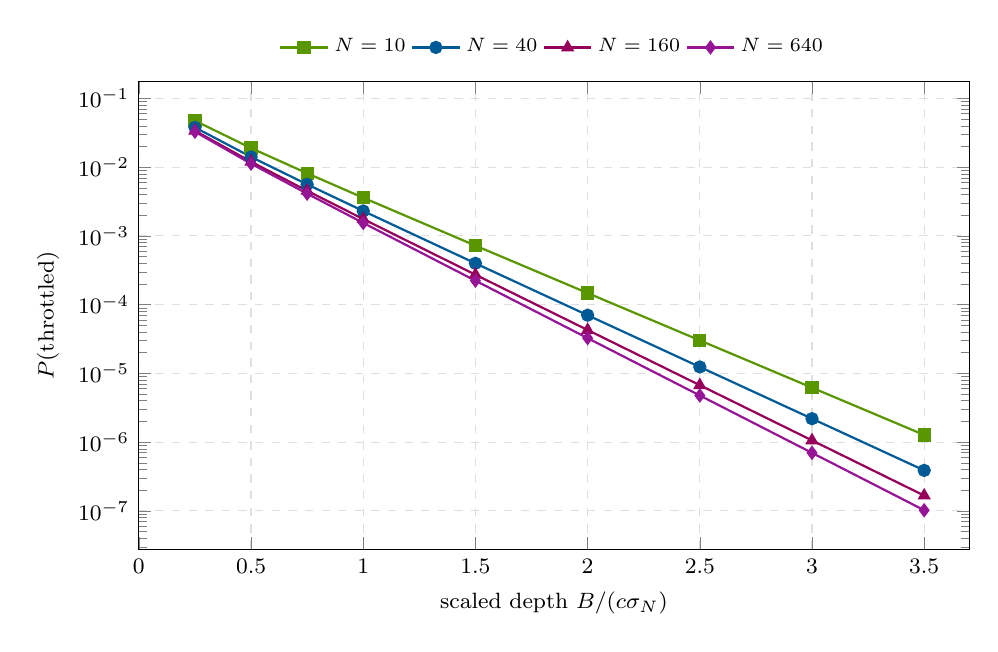
\begin{tikzpicture}
\begin{semilogyaxis}[width=\textwidth, height=0.62\textwidth, xmin=0, xmax=3.7,
  grid=major, grid style={gray!25},
  xlabel={scaled depth $B/(c\sigma_N)$}, ylabel={$P(\text{throttled})$}, legend style={at={(0.5,1.03)}, anchor=south, legend columns=4, font=\scriptsize},
  tick label style={font=\footnotesize}, label style={font=\footnotesize}]
\addplot[verdecito, thick, mark=square*] coordinates {(0.25,0.0474747) (0.5,0.0189984) (0.75,0.00815956) (1.0,0.0036) (1.5,0.000723228) (2.0,0.000147513) (2.5,3.02209e-05) (3.0,6.19836e-06) (3.5,1.27133e-06)};
\addlegendentry{$N=10$}
\addplot[azulcito, thick, mark=*] coordinates {(0.25,0.0379604) (0.5,0.0141119) (0.75,0.00562969) (1.0,0.00230657) (1.5,0.000399483) (2.0,7.02409e-05) (2.5,1.24055e-05) (3.0,2.19331e-06) (3.5,3.87727e-07)};
\addlegendentry{$N=40$}
\addplot[rojito, thick, mark=triangle*] coordinates {(0.25,0.0339638) (0.5,0.0120015) (0.75,0.00454124) (1.0,0.00176204) (1.5,0.000272858) (2.0,4.27948e-05) (2.5,6.73336e-06) (3.0,1.05979e-06) (3.5,1.66697e-07)};
\addlegendentry{$N=160$}
\addplot[violetita, thick, mark=diamond*] coordinates {(0.25,0.0328914) (0.5,0.0112607) (0.75,0.00412376) (1.0,0.00154687) (1.5,0.000223377) (2.0,3.26129e-05) (2.5,4.77229e-06) (3.0,6.98195e-07) (3.5,1.02044e-07)};
\addlegendentry{$N=640$}
\end{semilogyaxis}
\end{tikzpicture}

		\end{column}
		\begin{column}{0.42\textwidth}
			\begin{myitem}
				\item Margin fixed at $\beta=1$; quota in units of $c\,\sN$.
				\item As $N$ grows from $10$ to $640$, the curves \alert{settle}: throttling depends on $b$, not on $N$.
			\end{myitem}
			\vfill
			{\footnotesize Balance equations on a grid in $x$, checked against simulation. $\lambda=1$, $\nu=3$, $c=1$.}
		\end{column}
	\end{columns}
\end{frame}

\begin{frame}{The message}

	\vfill
	\begin{block}{}
		\begin{center}
		\large Overprovision the refill by order $\sqrt N$ above the mean burn,\\[0.3em]
		and a quota of order $\sqrt N$ suffices.
		\end{center}
	\end{block}
	\vfill
\end{frame}

%=====================================================================
\section{Conclusions}
%=====================================================================

\begin{frame}{Messages from the talk}

	\begin{myitem}[1.1em]
		\item A token quota shared by a fleet of agents is a \alert{flow-level token bucket}: a PDMP with state (active agents, tokens left).
		\item The \alert{empty bucket throttles} the fleet: a feedback fluid queue.
		\item Real spectrum from \alert{reversibility}.
		\item Existence, uniqueness and positivity from a \alert{$2\times2$ Perron--Frobenius} argument.
		\item \alert{Fluid limit}: full or empty; under-provisioning piles up the fleet above $\rho$.
		\item \alert{Square-root provisioning} (work in progress): a refill margin of order $\sqrt N$ above the mean burn, and a quota of order $\sqrt N$ suffices.
	\end{myitem}
\end{frame}


\begin{frame}{Future work}

	\begin{myitem}
		\item \alert{Heavy-tailed} token demands: tasks are far from exponential.
		\item \alert{Heterogeneous} agents, with different burn rates.
		\item \alert{Congestion}: crowded fleets may become less efficient, and burn more tokens per task.
		\item A proof of the \alert{diffusion limit}, and of the throttle decomposition.
	\end{myitem}
\end{frame}

\begin{frame}[plain]
	\vfill
	{\Huge \alert{Thank you!}}
	\vfill
	Andres Ferragut

	\smallskip

	\href{mailto://ferragut@ort.edu.uy}{\alert{ferragut@ort.edu.uy}}

	\smallskip

	\href{http://aferragu.github.io}{\alert{https://aferragu.github.io}}
\end{frame}

\begin{frame}[allowframebreaks]{References}
	\bibliography{tokens}
\end{frame}

%=====================================================================
\section*{Bonus track: exhaustion time}
%=====================================================================

\begin{frame}[plain]
	\vfill
	\begin{center}
		{\Huge \alert{Bonus track}}\\[1em]
		{\LARGE Token exhaustion time}
	\end{center}
	\vfill
\end{frame}

\begin{frame}{A quota that is never refilled}

	\begin{myitem}
		\item $p=0$: the fleet is \alert{autonomous} until the quota runs out.
		\item Tokens left: $x(t)=B-c\,A(t)$, with $A(t)=\int_0^t n(s)\,ds$ the \alert{agent-time}.
		\item Token exhaustion time: $T_B=\inf\{t: A(t)=B/c\}$. The level is hit \alert{exactly}: no overshoot.
		\item A completion time on a multimode system \cite{KNT1987}, for the Engset chain.
	\end{myitem}
\end{frame}

\begin{frame}{The mean exhaustion time}

	Linear rates give a linear eigenfunction:
	\begin{equation*}
		Q(n-\nb)=-\gamma(n-\nb),
	\end{equation*}
	hence a martingale, and by optional stopping:

	\vfill
	\pause

	\begin{proposition}
		\begin{equation*}
			\E{T_B} = \frac{1}{N\lambda}\left(\frac{\gamma B}{c} + \E{n(T_B)} - n(0)\right).
		\end{equation*}
	\end{proposition}

	\vfill
	\pause

	The only unknown is \alert{who is active} at exhaustion.
\end{frame}

\begin{frame}{Who is working when the quota runs out?}

	\begin{myitem}
		\item On the agent-time clock, $n$ is a Markov chain on $\{1,\ldots,N\}$.
		\item Its stationary law is \alert{size-biased}:
		\begin{equation*}
			\tilde\pi_n = \frac{n\,\pi_n}{\nb} \quad=\quad \text{law of } 1+\text{Bin}(N-1,\rho).
		\end{equation*}
	\end{myitem}

	\vfill
	\pause

	\begin{block}{}
		\begin{center}
		At the instant the last token is spent, \alert{some agent is spending it}.\\
		The other $N-1$ are active independently with probability $\rho$: an \alert{arrival theorem}.
		\end{center}
	\end{block}
\end{frame}

\begin{frame}{Back to the mean}

	\begin{myitem}
		\item For large $B$:
		\begin{equation*}
			\E{T_B} \approx \frac{B}{c\nb} + \frac{\nb + (1-\rho) - n(0)}{N\lambda}.
		\end{equation*}
		\item<2-> If $n(0)$ is drawn from the size-biased law, the correction vanishes, \alert{exactly}:
		\begin{equation*}
			\E{T_B} = \frac{B}{c\nb}\quad\text{for every } B.
		\end{equation*}
	\end{myitem}
\end{frame}


\end{document}
